\chapter{Symulacyjna weryfikacja tezy}

Weryfikacja przedstawionego w pracy modelu błędu i wynikających z niego założeń w pierwszej kolejności przeprowadzona została metodą symulacyjną. W bieżącym rozdziale przedstawiono przykładowy tor pomiarowy, a następnie wymieniono i opisano obecne w nim źródła błędów. Na podstawie przedstawionego wcześniej modelu błędu opisano związki zachodzące pomiędzy zidentyfikowanymi sygnałami błędów oraz oszacowano wartości niepewności rozszerzonych wielkości wyjściowych analizowanego toru pomiarowego. Wyniki uzyskane za pomocą zaproponowanego modelu porównano z wynikami uzyskanymi metodą Monte-Carlo. W celu możliwości bieżącej weryfikacji poprawności stosowanych założeń, podczas analizy wyznaczano wartości dla wszystkich wyprowadzanych wielkości, które umożliwiły porównanie uzyskanych wyników z wynikami symulacji metodą Monet-Carlo. Przedstawione wyniki liczbowe przedstawiano jedynie w celu możliwości weryfikacji każdego etapu analizy, natomiast ostateczne wyniki wyznaczane były na podstawie wyprowadzonych wcześniej zależności.

Przykładowy tor pomiarowy składa się z przetwornika pomiarowego, który przekształca ciągłą w czasie wielkość fizyczną $s(t)$ na reprezentujący ją sygnał napięciowy $y_{a}(t)$. Sygnał wyjściowy przetwornika pomiarowego poddawany jest wzmocnieniu w celu dopasowania jego poziomu do zakresu napięcia wejściowego przetwornika analogowo-cyfrowego. Wzmocniony sygnał $y_{b}(t)$ stanowi wejście przetwornika analogowo-cyfrowego, którego wielkości wyjściowe oznaczono symbolem $x_{c}(i)$. Ostatecznie sygnał wyjściowy przetwornika analogowo-cyfrowego trafia na wejście algorytmu dyskretnej transformacji falkowej, a na jego podstawie wyznaczany jest wektor wielkości wyjściowych, oznaczonych jako $X(k)$. Schemat ideowy opisanego toru pomiarowego przedstawiono na rysunku~\ref{fig:chain_symul}.

\begin{figure}[htb!]
\begin{center}
\includegraphics{obrazki/schemat_symul}
\makecaption{fig:chain_symul}{Schemat blokowy toru pomiarowego będącego obiektem przeprowadzanego eksperymentu symulacyjnego}
\end{center}
\end{figure}

Podczas eksperymentu przyjęto, że przetwarzany sygnał pomiarowy obarczony jest błędem związanym z szumem białym o stałej widmowej gęstości mocy. Przetwornik pomiarowy, zastosowany w celu przetworzenia analizowanego sygnału wejściowego na postać napięciową, cechuje się pewną częstotliwość graniczną, a jego charakterystyka nie jest idealnie liniowa. Zastosowany wzmacniacz pomiarowy również charakteryzuje się pewną częstotliwością graniczną, natomiast założono, że nieliniowość charakterystyki jest w jego przypadku pomijalnie mała. Przyjęto, że temperatura otoczenia miała wpływ na dryf zera przetwornika pomiarowego oraz wzmacniacza, przy czym temperatura ta nie była mierzona, zatem jej wpływ na wyniki pomiarów nie był korygowany. Przyjęto, że zastosowany przetwornik analogowo-cyfrowy wprowadzał do sygnału wyjściowego jedynie błąd związany z kwantowaniem przetwarzanej wielkości, natomiast algorytm transformacji falkowej wprowadzał do wielkości wyjściowych błąd własny związany z wykonywaniem operacji na liczbach zmiennoprzecinkowych.

W dalszej części rozdziału omówiono kolejne elementy toru pomiarowego, wskazano ich wpływ na przetwarzany sygnał oraz relacje pomiędzy sygnałami błędów na wejściu i wyjściu tych fragmentów. Przedstawiono również szczegółowe założenia odnośnie właściwości opisanych we wprowadzeniu fragmentów toru pomiarowego. Dla przeprowadzonego eksperymentu przyjęto, że przetwarzany sygnał $s(t)$ określony został w dziedzinie czasu jako:
\begin{gather}
\dot{s} \emb{t} = \frac{6}{10} \sin \left( 2 \pi f_{1} t \right) - \frac{3}{10} \sin \left( 10 \pi f_{1} t + \frac{\pi}{8} \right) + \frac{1}{10} \sin \left( 30 \pi f_{1} t + \frac{\pi}{6} \right) \label{eq:sym_in_ideal}, \\
\tilde{s} \emb{t} = \dot{s} \emb{t} + e_{s,r} \emb{t} = e_{s,r} \emb{t} + \sum _{i=1} ^{3} E_{s,o} \emb{\omega_{s,i}} \sin \emb{\omega_{s,i} t + \varphi_{s,i}} \label{eq:sym_in_real},
\end{gather}
przy czym $f_{1} = \qty{1}{kHz}$ jest częstotliwością podstawowej harmonicznej tego sygnału, natomiast $\sigma_{s,r}^{2}(\omega) = \frac{2}{3} \cdot 10^{-5}$ wariancją sygnału szumu $e_{s,r}(t)$. Parametry kolejnych harmonicznych przetwarzanego sygnału zostały zestawione w tabeli~\ref{tab:sym_in_params_ideal}. Do wyznaczenia wektora wielkości wyjściowych algorytmu dyskretnej transformacji falkowej koniecznych było $N = 8$ próbek wielkości wejściowych $x_{c}(i)$ tego algorytmu, na podstawie których wyznaczano $M = 8$ próbek wielkości wyjściowych $X(k)$ obiektu dla każdej realizacji pomiaru. Eksperyment zakładał stały dla każdej próbki przetwarzanego sygnału okres próbkowania, który wynosił $f_{s} = \qty{48}{kHz}$, natomiast okno pomiarowe usytuowane było losowo względem przebiegu przetwarzanego sygnału $s(t)$. Dodatkowo założono, że temperatura otoczenia przyjmowała dowolną wartość z zakresu $\hat{\vartheta}(t)\in~<17;23>\unit{\degreeCelsius}$, wartością oczekiwaną temperatury była wartość~\qty{20}{\degreeCelsius} oraz w obrębie wskazanego przedziału rozkład wartości temperatury był rozkładem trójkątnym.

\begin{table}[htb!]
\begin{center}
\makecaption{tab:sym_in_params_ideal}{Parametry kolejnych harmonicznych przetwarzanego sygnału przyjęte w przeprowadzanym eksperymencie symulacyjnym dla sytuacji idealnej}
\begin{tabular}[c]{| c | c | c | c |} \hline
\textbf{Lp. $i$} & \textbf{Pulsacja $\omega_{s,i}$, rad/s} & \textbf{Amplituda $E_{s,o}(\omega_{s,i})$} & \textbf{Faza $\varphi_{s,o}(\omega_{s,i})$, rad} \\ \hline
1 & $1000  \cdot 2\pi$ &  \num{0.6} & $0$           \\ \hline
2 & $5000  \cdot 2\pi$ &  \num{0.3} & $\pi/8 + \pi$ \\ \hline
3 & $15000 \cdot 2\pi$ &  \num{0.1} & $\pi/6$       \\ \hline
\end{tabular}
\end{center}
\end{table}

\section{Analiza przetwornika pomiarowego}

Zastosowany w przykładzie przetwornik pomiarowy przekształca sygnał $s(t)$, związany z mierzoną wielkością fizyczną, na wyjściowy sygnał napięciowy $y_{a}(t)$. Przyjmuje się, że mierzona wielkość zmieniać się może w zakresie $\hat{s}(t) \in~<0;1>$, przy czym czułość przetwornika pomiarowego jest równa $s_{a} = \qty{1}{V \per 1}$, a jego częstotliwość graniczna wynosi $f_{a,g} = \qty{320}{kHz}$. Wobec powyższych, wartość wielkości wyjściowej $y_{a}(t)$ mieści się w przedziale $\hat{y}_{a}(t) \in~<0;1>\unit{V}$. Charakterystyka omawianego obiektu jest zależna od temperatury otoczenia, przy czym temperatura ta nie jest znana.

Stosując zaproponowany model błędu i przedstawione założenia, na podstawie równań~\eqref{eq:out_cont_ideal_all} oraz~\eqref{eq:out_cont_real_all}, opisać można przebieg wielkości wyjściowej $y_{a}(t)$ jako:
\begin{gather}
\dot{y}_{a} \emb{t} = \dot{f}_{a} \emb{\dot{s} \emb{t}} = \dot{s} \emb{t} \label{eq:sym_parta_out_ideal}, \\
\tilde{y}_{a} \emb{t} = \dot{y}_{a} \emb{t} + e_{a,\Sigma} \emb{t} \label{eq:sym_parta_out_real},
\end{gather}
przy czym sygnały błędów zawarte w sygnale błędu wypadkowego $e_{a,\Sigma}(t)$ zdefiniowano i omówiono w dalszej cześć podrozdziału. Funkcja przetwarzania obiektu $f_{a}(x)$ powinna być zatem w przypadku idealnym, zgodnie z założeniami opisanymi zależnością~\eqref{eq:sym_parta_out_ideal} oraz wymienionymi we wstępie podrozdziału, określona równaniem w postaci:
\begin{equation}
\dot{f}_{a} \emb{x} = s_{a} x = x \label{eq:sym_parta_statfun}.
\end{equation}
Przyjmuje się, że rzeczywista funkcja przetwarzania obiektu $\tilde{f}_{a}(x)$ nie jest znana, natomiast realizacje sygnału błędu $e_{a,zw}(t)$ wynikającego z nieliniowości charakterystyki przyjmują wartości z przedziału $\hat{e}_{a,fw}(t) \in~<-\sqrt{10};\sqrt{10}>\unit{mV}$, a uzyskanie każdej z nich jest jednakowo prawdopodobne. Przyjmuje się, że charakter rozważanego sygnału błędu jest zbliżony do charakteru sygnału błędu kwantowania, zatem błąd ten zaliczyć można do grupy błędów losowych. Wariancję oraz niepewność rozszerzoną, związane z omawianym sygnałem błędu $e_{a,rw}(t) = e_{a,fw}(t)$, wyrazić można w postaci~\cite{jcgm_guide}:
\begin{gather}
\sigma_{a,rw}^{2} = \frac{\left( \left( \sqrt{10} \cdot 10^{-3} \right) + \left( \sqrt{10} \cdot 10^{-3} \right) \right)^{2}}{12} = 3 \frac{1}{3}~\unit{\micro V} \label{eq:sym_parta_rand_self_var}, \\
U_{a,rw} = c_{u} \sigma_{a,rw} = \frac{\num{1.65} \sqrt{30}}{3}~\unit{mV} \label{eq:sym_parta_rand_self_unc},
\end{gather}
przy czym $c_{u}$ jest współczynnikiem rozszerzenia dla rozkładu jednostajnego i przy poziomie ufności $\alpha = \qty{95}{\percent}$ wynosi~\num{1.65}. Ze względu na nieznaną postać rzeczywistej funkcji przetwarzania, w dalszych rozważaniach przyjmuje się, że $\tilde{f}_{a}(x)  \cong  \dot{f}_{a}(x)$.

Zmiany temperatury otoczenia ujęte w założeniach eksperymentu deklarowane były jako bardzo niewielkie w obrębie pojedynczej serii pomiarowej. Można zatem przyjąć, że błąd wynikający z wpływu tej temperatury na wartość wielkości wyjściowej analizowanego obiektu jest niezmienny w obrębie pojedynczego okna pomiarowego, a zatem, zgodnie z przyjętym modelem, kwalifikować go można jako błąd statyczny. Przyjmuje się wobec tego, że sygnał błędu statycznego własnego związany z omawianym zjawiskiem, zgodnie z równaniem~\eqref{eq:out_cont_err_env_self}, jest określony jako:
\begin{equation}
e_{a,sw} \emb{t} = f_{a,z} \left( \vartheta \emb{t} \right) = \frac{3}{2} \left( \vartheta \emb{t} - \qty{20}{\degreeCelsius} \right)~\unit{\frac{mV}{K}} \label{eq:sym_parta_stat_err},
\end{equation}
gdzie $\vartheta(t)$ jest rzeczywistą temperaturą otoczenia wyrażoną w stopniach Celsjusza. Można zatem określić wariancję oraz niepewność rozszerzoną omawianego sygnału~\cite{jcgm_guide}:
\begin{gather}
\sigma_{a,sw}^{2} = \frac{\left( -\frac{9}{2} \cdot 10^{-3} \right)^{2} + \left( \frac{9}{2} \cdot 10^{-3} \right)^{2} - \left( -\frac{9}{2} \cdot 10^{-3} \right) \left( \frac{9}{2} \cdot 10^{-3} \right)}{18} = 3 \frac{3}{8}~\unit{\micro V} \label{eq:sym_parta_stat_var}, \\
U_{a,sw} = c_{t} \sigma_{a,rw} = \frac{\num{5.7} \sqrt{6}}{4}~\unit{mV} \label{eq:sym_parta_stat_unc},
\end{gather}
gdzie $c_{t}$ jest współczynnikiem rozszerzenia dla rozkładu trójkątnego i przy poziomie ufności $\alpha = \qty{95}{\percent}$ wynosi~\num{1.90}.

Kolejną grupę właściwości obiektu stanowią właściwości dynamiczne, związane z jego częstotliwością graniczną. Przypadek idealny zakłada, że analizowany obiekt nie powinien mieć żadnego wpływu na widmo przetwarzanego sygnału, a zatem transmitancja tego obiektu powinna wynosić $\dot{G}_{a}(j\omega) = 1$. Na podstawie założonych parametrów rzeczywistych obiektu przyjmuje się, że transmitancja $\tilde{G}_{a}(j\omega)$ wynosi:
\begin{equation}
\tilde{G}_{a} \emb{j\omega} = \frac{1}{1 + j \frac{\omega}{2 \pi f_{a,g}}} = \frac{1}{\frac{\omega^{2}}{4 \pi^{2} f_{a,g}^{2}} + 1} - j \frac{\omega}{2 \pi f_{a,g} \left( \frac{\omega^{2}}{4 \pi^{2} f_{a,g}^{2}} + 1 \right) } \label{eq:sym_parta_trans},
\end{equation}
zatem równania~\eqref{eq:mid_cont_amp} oraz~\eqref{eq:mid_cont_phi}, określające właściwości dynamiczne, przyjmują postać:
\begin{gather}
\tilde{K}_{a} \emb{\omega} = \sqrt{\left( \Re \left( \tilde{G}_{a} \emb{j\omega} \right) \right)^{2} + \left( \Im \left( \tilde{G}_{a} \emb{j\omega} \right) \right)^{2}} = \left( \frac{\omega^{2}}{4 \pi^{2} f_{a,g}^{2}} + 1 \right)^{-\frac{1}{2}} \label{eq:sym_parta_amp_real}, \\
\tilde{\varphi}_{a} \emb{\omega} = \arctan \left( \frac{\Im \left( \tilde{G}_{a} \emb{j\omega} \right)}{\Re \left( \tilde{G}_{a} \emb{j\omega} \right)} \right) = \arctan \left( -\frac{\omega}{2 \pi f_{a,g}} \right) \label{eq:sym_parta_phi_real}, \\
\dot{K}_{a} \emb{\omega} = \sqrt{\left( \Re \left( \dot{G}_{a} \emb{j\omega} \right) \right)^{2} + \left( \Im \left( \dot{G}_{a} \emb{j\omega} \right) \right)^{2}} = 1 \label{eq:sym_parta_amp_ideal}, \\
\dot{\varphi}_{a} \emb{\omega} = \arctan \left( \frac{\Im \left( \dot{G}_{a} \emb{j\omega} \right)}{\Re \left( \dot{G}_{a} \emb{j\omega} \right)} \right) = 0 \label{eq:sym_parta_phi_ideal}.
\end{gather}

Na podstawie powyższych zależności określających parametry transmitancji obiektu w sytuacji idealnej, a także założeń~\eqref{eq:mid_cont_omega_ideal}, \eqref{eq:mid_cont_sum_ideal}, \eqref{eq:out_cont_ideal_all} oraz~\eqref{eq:sym_parta_out_ideal}, opisać można idealne parametry kolejnych harmonicznych sygnału $y_{a}(t)$ w funkcji pulsacji jako:
\begin{gather}
E_{a,o} \emb{\omega} = \dot{f}_{a} \emb{\dot{K}_{a} \emb{\omega} E_{s,o} \emb{\omega}} = E_{s,o} \emb{\omega} \label{eq:sym_parta_amp_out_ideal}, \\
\varphi_{a,o} \emb{\omega} = \varphi_{s,o} \emb{\omega} + \dot{\varphi}_{a} \emb{\omega} = \varphi_{s,o} \emb{\omega} \label{eq:sym_parta_phi_out_ideal},
\end{gather}
gdzie $E_{a,o}(\omega)$ jest idealną amplitudą oraz $\varphi_{a,o}(\omega)$ idealną fazą harmonicznej sygnału wyjściowego $y_{a}(t)$ o wybranej pulsacji. Wskazane zależności oraz definicja przetwarzanego sygnału wejściowego, dana równaniem~\eqref{eq:sym_in_ideal}, umożliwiają definicję opisanej równaniem~\eqref{eq:sym_parta_out_ideal} wielkości wyjściowej obiektu dla przypadku idealnego w postaci sumy analizowanych harmonicznych tego sygnału:
\begin{equation}
\dot{y}_{a} \emb{t} = \sum _{i=1} ^{3} E_{a,o} \emb{\omega_{a,i}} \sin \emb{\omega_{a,i} t + \varphi_{a,i}} \label{eq:sym_parta_out_ideal_sum},
\end{equation}
przy czym $\omega_{a,i} = \omega_{s,i}$ jest pulsacją $i$-tej harmonicznej sygnału wyjściowego, której kolejne wartości zestawione zostały wcześniej w tabeli~\ref{tab:sym_in_params_ideal}. Parametry sygnału opisanego równaniem~\eqref{eq:sym_parta_out_ideal_sum} zestawiono w tabeli~\ref{tab:sym_outa_params_ideal}.

\begin{table}[htb!]
\begin{center}
\makecaption{tab:sym_outa_params_ideal}{Parametry kolejnych harmonicznych sygnału $y_{a}(t)$ przyjęte w przeprowadzanym eksperymencie symulacyjnym dla sytuacji idealnej}
\begin{tabular}[c]{| c | c | c | c |} \hline
\textbf{Lp. $i$} & \textbf{Pulsacja $\omega_{a,i}$, rad/s} & \textbf{Amplituda $E_{a,o}(\omega_{a,i})$, V} & \textbf{Faza $\varphi_{a,o}(\omega_{a,i})$, rad} \\ \hline
1 & $1000  \cdot 2\pi$ &  \num{0.6} & $0$             \\ \hline
2 & $5000  \cdot 2\pi$ &  \num{0.3} & $\pi/8 + \pi$   \\ \hline
3 & $15000 \cdot 2\pi$ &  \num{0.1} & $\pi/6$         \\ \hline
\end{tabular}
\end{center}
\end{table}

Na podstawie równań~\eqref{eq:mid_cont_err_dyn_self} oraz~\eqref{eq:out_cont_err_dyn_self}, błąd własny dynamiczny w funkcji pulsacji wybranej harmonicznej sygnału opisać można następującą zależnością:
\begin{equation}
\begin{split}
e_{a,dw} \emb{t,\omega} =~
& \tilde{f}_{a} \emb{\tilde{K}_{a} \emb{\omega} E_{s,o} \emb{\omega} \sin \left( \omega t + \varphi_{s,o} \emb{\omega} + \tilde{\varphi}_{a} \emb{\omega} \right)} - \\
& \tilde{f}_{a} \emb{\dot{K}_{a} \emb{\omega} E_{s,o} \emb{\omega} \sin \left( \omega t + \varphi_{s,o} \emb{\omega} + \dot{\varphi}_{a} \emb{\omega} \right)}
\end{split}
\label{eq:sym_parta_dyn_self_err}.
\end{equation}
Jako, że sygnał wejściowy $s(t)$ analizowanego obiektu nie jest obarczony błędem dynamicznym, nie ma potrzeby wykonywania analizy dla sygnału błędu dynamicznego propagowanego. Aby umożliwić analizę propagacji sygnałów błędów dynamicznych przez kolejne fragmenty toru pomiarowego, minimalizując jednocześnie liczbę analizowanych składowych błędu dynamicznego, wyznaczono na podstawie równań~\eqref{eq:dyn_vect_amp} oraz~\eqref{eq:dyn_vect_phi} wypadkowe parametry amplitudy oraz fazy dla kolejnych harmonicznych tego sygnału. Należy zauważyć, że relacje pomiędzy amplitudą, a wariancją analizowanej harmonicznej opisuje równanie~\eqref{eq:dyn_var}. Analizując równanie~\eqref{eq:sym_parta_dyn_self_err} można zauważyć, że dla każdej harmonicznej błąd ten ma dwie składowe o przeciwnych znakach. Korzystając z właściwości funkcji \enquote{sinus} można odwrócić znak wybranej składowej oraz dodać kąt $\pi~\unit{rad}$ do argumentu tej funkcji, zachowując przy tym oryginalną wartość tej składowej.

Stosując podane założenia, przebieg składowej sygnału błędu dynamicznego własnego o częstotliwości~\qty{1}{kHz} przedstawić można następującym równaniem:
\begin{equation}
\begin{split}
e_{a,dw} \emb{t,\omega} \left|_{\omega = 1000 \cdot 2 \pi } \right. =~
& \tilde{f}_{y} \emb{\tilde{K}_{a} \emb{\omega} E_{s,o} \emb{\omega} \sin \left( \omega t + \varphi_{s,o} \emb{\omega} + \tilde{\varphi}_{a} \emb{\omega} \right)} - \\
& \tilde{f}_{y} \emb{\dot{K}_{a} \emb{\omega} E_{s,o} \emb{\omega} \sin \left( \omega t + \varphi_{s,o} \emb{\omega} + \dot{\varphi}_{a} \emb{\omega} \right)} = \\
& \num{1.0} \cdot \num{0.6} \sin \left( 1000 \cdot 2 \pi t + 0 - \num{3.13e-3} \right) + \\
& \num{1.0} \cdot \num{0.6} \sin \left( 1000 \cdot 2 \pi t + 0 + 0 + \pi \right)
\end{split}
\label{eq:sym_parta_dyn_self_example_harm},
\end{equation}
przy czym opisane w podany sposób parametry kolejnych harmonicznych sygnału błędu dynamicznego zestawiono w tabeli~\ref{tab:sym_parta_params_dyn_list}. Przedstawiając składowe równania~\eqref{eq:sym_parta_dyn_self_example_harm} za pomocą wektorów, zgodnie z równaniem~\eqref{eq:dyn_vect}, a następnie zgodnie z równaniem~\eqref{eq:dyn_vect_sum} sumując opisane składniki, wyznaczyć można wypadkowe parametry harmonicznych sygnału błędu zgodnie z zależnościami~\eqref{eq:dyn_vect_amp} oraz~\eqref{eq:dyn_vect_phi}. Dla przedstawionej w równaniu~\eqref{eq:sym_parta_dyn_self_example_harm} harmonicznej sygnału błędu dynamicznego, parametry te wynoszą:
\begin{gather}
\mathbf{e}_{a,e,1} =
\begin{bmatrix}
\num{0.6} \cos \emb{\num{-3.13e-3}} + \num{0.6} \cos \emb{\pi} & \num{0.6} \sin \emb{\num{-3.13e-3}} + \num{0.6} \sin \emb{\pi}
\end{bmatrix}
\label{eq:sym_parta_dyn_self_example_sum}, \\
E_{\Sigma,a,e,1} = \sqrt{\emb{\num{-5.86e-6}}^{2} + \emb{\num{-1.88e-3}}^{2}} = \qty{1.88}{mV} \label{eq:sym_parta_dyn_self_example_amp}, \\
\varphi_{\Sigma,a,e,1} = \arctan \emb{\frac{\num{-1.88e-3}}{\num{-5.86e-6}}} = \qty{-1.57}{rad} \label{eq:sym_parta_dyn_self_example_phi}.
\end{gather}
Dla pozostałych harmonicznych należy opisane powyżej wielkości wyznaczyć w sposób analogiczny, przy czym wartości tych wielkości zestawiono w tabeli~\ref{tab:sym_parta_params_dyn_summary}. Na podstawie równania~\eqref{eq:dyn_var} możliwe jest wyznaczenie wartości wariancji kolejnych składowych błędu dynamicznego oraz na podstawie równania~\eqref{eq:unc_sum} wartości ich niepewności rozszerzonej:
\begin{gather}
\sigma_{a,dw,1}^{2} = \frac{E_{a,e,1}^{2}}{2} = \qty{1.77}{\micro V} \label{eq:sym_parta_dyn_self_var}, \\
U_{a,dw,1} = c_{d} \sigma_{a,rw} = \qty{1.87}{mV} \label{eq:sym_parta_dyn_self_unc},
\end{gather}
przy czym dla rozkładu dwumodalnego współczynnik rozszerzenia $c_{d}$ dla deklarowanego poziomu ufności $\alpha = \qty{95}{\percent}$ jest równy~\num{1.42}~\cite{jakubiec_system}.

\begin{table}[htb!]
\begin{center}
\makecaption{tab:sym_parta_params_dyn_list}{Parametry składowe kolejnych harmonicznych błędu dynamicznego własnego analizowanego w eksperymencie symulacyjnym przetwornika pomiarowego}
\begin{tabular}[c]{| c | c | c | c |} \hline
\textbf{Lp. $i$} & \textbf{Pulsacja $\omega_{a,i}$, rad/s} & \textbf{Amplituda $E_{a,e}(\omega_{a,i})$, V} & \textbf{Faza $\varphi_{a,e}(\omega_{a,i})$, rad} \\ \hline
1 & \multirow{2}{*}{$1000  \cdot 2\pi$} &  $\num{1.0} \cdot \num{0.6}$       & $0 - \num{3.13e-3}$            \\ \cline{1-1} \cline{3-4}
2 &                                     &  $\num{1.0} \cdot \num{0.6}$       & $0 + 0 + \pi$                  \\ \hline
3 & \multirow{2}{*}{$5000  \cdot 2\pi$} &  $\num{1.0} \cdot \num{0.3}$       & $\pi/8 - \num{1.56e-2} + \pi$  \\ \cline{1-1} \cline{3-4}
4 &                                     &  $\num{1.0} \cdot \num{0.3}$       & $\pi/8 + 0$                    \\ \hline
5 & \multirow{2}{*}{$15000 \cdot 2\pi$} &  $\num{1.0} \cdot \num{0.1}$       & $\pi/6 - \num{4.69e-2}$        \\ \cline{1-1} \cline{3-4}
6 &                                     &  $\num{1.0} \cdot \num{0.1}$       & $\pi/6 + 0 + \pi$              \\ \hline
\end{tabular}
\end{center}
\end{table}

\begin{table}[htb!]
\begin{center}
\makecaption{tab:sym_parta_params_dyn_summary}{Parametry wypadkowe kolejnych harmonicznych błędu dynamicznego własnego analizowanego w eksperymencie symulacyjnym przetwornika pomiarowego}
\begin{tabular}[c]{| c | c | S[table-format = 1.2] | S[table-format = +1.2] |} \hline
\textbf{Lp. $j$} & \textbf{Pulsacja $\omega_{a,j}$, rad/s} & \textbf{Amplituda $E_{a,e}(\omega_{a,j})$, mV} & \textbf{Faza $\varphi_{a,e}(\omega_{a,j})$, rad} \\ \hline
1 & $1000  \cdot 2\pi$  &  1.88  & -1.57  \\ \hline
2 & $5000  \cdot 2\pi$  &  4.69  &  1.96  \\ \hline
3 & $15000 \cdot 2\pi$  &  4.68  & -1.07  \\ \hline
\end{tabular}
\end{center}
\end{table}

Wyprowadzone dotychczas zależności oraz dane zestawione w tabeli~\ref{tab:sym_parta_params_dyn_summary} pozwalają, zgodnie z równaniem~\eqref{eq:mid_cont_err_dyn_self} zdefiniować wypadkowy sygnał błędu dynamicznego własnego w postaci sumy kolejnych harmonicznych tego sygnału:
\begin{equation}
e_{a,dw} \emb{t} = \sum _{j=1} ^{3} E_{a,e} \emb{\omega_{a,e}} \sin \emb{\omega_{a,j} t + \varphi_{a,e} \emb{\omega_{a,j}}} \label{eq:sym_parta_dyn_self_sum}.
\end{equation}
Należy zauważyć, że ze względu na fakt, że sygnał ten będzie przetwarzany przez kolejne fragmenty toru pomiarowego, dalsza analiza wykorzystująca wypadkowe parametry kolejnych harmonicznych tego sygnału wydaje się być najbardziej przystępna.

Ostatnim sygnałem błędu wymagającym analizy jest sygnał $e_{a,rp}(t)$, związany z szumem na wejściu obiektu. Wariancję tego sygnału w funkcji pulsacji określić można stosując kolejno zależności~\eqref{eq:mid_cont_var_omega} oraz~\eqref{eq:out_cont_var_sense}, a zatem zapisać można:
\begin{equation}
\sigma_{a,rp}^{2} \emb{\omega} = s_{a}^{2} \tilde{K}_{a}^{2} \emb{\omega} \sigma_{s,r}^{2} \emb{\omega} \cong \sigma_{s,r}^{2} \emb{\omega} = \frac{20}{3}~\unit{\micro V} \label{eq:sym_parta_rand_prop_var_omega}.
\end{equation}
Zauważyć można, że w zakresie częstotliwości $\hat{f} \in~<0;\frac{1}{2} f_{p}>$ wartość wzmocnienia $\tilde{K}_{a}(\omega)$ jest zbliżona do jedności, a zatem transmitancja obiektu nie wpływa na widmo przetwarzanego sygnału szumu. Można zatem przyjąć, że wariancja sygnału błędu losowego propagowanego w funkcji pulsacji jest identyczna, jak na wejściu obiektu dla analizowanego zakresu częstotliwości. Niepewność rozszerzoną związaną z opisywanym sygnałem wyznaczyć można zatem, zgodnie z zależnością~\eqref{eq:unc_sum}, w postaci:
\begin{equation}
U_{a,rp} = c_{u} \sigma_{a,rp} = \frac{\num{3.92} \sqrt{15}}{3}~\unit{mV} \label{eq:sym_parta_rand_prop_unc},
\end{equation}
gdzie $c_{u}$ to współczynnik rozszerzenia rozkładu normalnego, równy~\num{1.96} dla $\alpha = \qty{95}{\percent}$.

Zdefiniowane dotychczas sygnały błędów stanowią kolejne składniki wypadkowego sygnału błędu $e_{a,\Sigma}(t)$ wielkości wyjściowej analizowanego obiektu, wprowadzonego wcześniej w równaniu~\eqref{eq:sym_parta_out_real}. Ostatecznie, sygnał ten opisać można w postaci:
\begin{equation}
e_{a,\Sigma} \emb{t} = e_{a,sw} \emb{t} + e_{a,rw} \emb{t} + e_{a,rp} \emb{t} + e_{a,dw} \emb{t} \label{eq:sym_parta_error_sum}.
\end{equation}
Na podstawie parametrów wymienionych sygnałów określono budżet niepewności dla analizowanego fragmentu toru pomiarowego, który zestawiono w tabeli~\ref{tab:sym_parta_params_unc_list}. Należy zauważyć, że kolejne sygnały błędów w opisywanym przypadku nie są skorelowane.

\begin{table}[htb!]
\begin{center}
\makecaption{tab:sym_parta_params_unc_list}{Budżet niepewności wielkości wyjściowej analizowanego w eksperymencie symulacyjnym przetwornika pomiarowego}
\begin{tabular}[c]{| c | c | S[table-format = 1.2] | S[table-format = 2.2] | c | c |} \hline
\textbf{Lp.} & \textbf{Symbol} & \textbf{$U$, mV} & \textbf{$\sigma^{2}$, \micro V} & \textbf{Rozkład} & \textbf{Źródło błędu} \\ \hline
1 & ${a,sw}$       & 3.49  &  3.38   & trójkątny                    & dryf temperatury                           \\ \hline
2 & ${a,rw}$       & 3.01  &  3.33   & jednostajny                  & nieliniowość obiektu                       \\ \hline
3 & ${a,rp}$       & 5.06  &  6.67   & normalny                     & szum wielkości wejściowej                  \\ \hline
4 & ${a,dw,1}$     & 1.87  &  1.77   & \multirow{3}{*}{dwumodalny}  & \multirow{3}{*}{transmitancja wzmacniacza} \\ \cline{1-4}
5 & ${a,dw,2}$     & 4.68  &  11.00  &                              &                                            \\ \cline{1-4}
6 & ${a,dw,3}$     & 4.67  &  10.95  &                              &                                            \\ \hline
\end{tabular}
\end{center}
\end{table}

Ostatnim możliwym krokiem pozostaje zatem określenie wypadkowej wartości niepewności rozszerzonej dla analizowanego fragmentu toru pomiarowego. Na obecnym etapie rozważań wyznaczanie tego parametru nie jest konieczne i nie będzie wykorzystywane w dalszym procesie analizy -- przeprowadzenie tej operacji jest jednak uzasadnione potrzebą weryfikacji skuteczności proponowanej metody wyznaczania wypadkowej wartości niepewności rozszerzonej, opisanej równaniem~\eqref{eq:unc_matrix}.

Uwzględniając podział rodzajów sygnałów błędów zorientowany ze względu na charakter ich realizacji, równanie~\eqref{eq:sym_parta_error_cat} zapisać można również w postaci:
\begin{gather}
e_{a,\Sigma} \emb{t} = e_{a,s} \emb{t} + e_{a,d} \emb{t} + e_{a,r} \emb{t} \label{eq:sym_parta_error_cat}. \\
e_{a,s} \emb{t} = e_{a,sw} \emb{t} \label{eq:sym_parta_error_stat}, \\
e_{a,d} \emb{t} = e_{a,dw} \emb{t} \label{eq:sym_parta_error_dyn}, \\
e_{a,s} \emb{t} = e_{a,rw} \emb{t} + e_{a,rp} \emb{t} \label{eq:sym_parta_error_rand},
\end{gather}
gdzie $e_{a,s}(t)$ jest wypadkowym sygnałem błędu statycznego, $e_{a,d}(t)$ dynamicznego, natomiast $e_{a,r}(t)$ losowego. W przypadku sygnału błędu statycznego $e_{a,s}(t)$, ze względu na istnienie tylko jednego źródła tego błędu, zapisać można:
\begin{gather}
U_{a,s} = U_{a,sw} = \qty{3.49}{mV} \label{eq:sym_parta_uncert_stat}, \\
\sigma_{a,s}^{2} = \sigma_{a,sw}^{2} = \qty{3.38}{\micro V} \label{eq:sym_parta_var_stat}.
\end{gather}
Dla sygnałów błędu dynamicznego $e_{a,d}(t)$ oraz losowego $e_{a,r}(t)$ wypadkowe wartości niepewności rozszerzonej szacowane są zgodnie z równaniem~\eqref{eq:unc_matrix}, przy czym kolejne wartości współczynników koherencji wyznaczane są zgodnie z zależnością~\eqref{eq:unc_coher}. Ze względu na brak korelacji pomiędzy analizowanymi składnikami sygnałów błędów, wypadkowe wartości wariancji mogą być wyznaczane zgodnie z równaniem~\eqref{eq:var_sum}. Po oszacowaniu wartości parametrów wypadkowych niepewności rozszerzonych oraz wariancji, wartości współczynników rozszerzenia mogą być oszacowane zgodnie z równaniem~\eqref{eq:unc_sum}. Wymienione zależności przyjmują w bieżącym przypadku postać:
\begin{gather}
\begin{split}
U_{a,d} = ~ & \sqrt{
\begin{bmatrix}
U_{a,dw,1} \\ U_{a,dw,2} \\ U_{a,dw,3}
\end{bmatrix}^{T}
\begin{bmatrix}
1            & h_{a,dw,1,2} & h_{a,dw,1,3} \\
h_{a,dw,2,1} & 1            & h_{a,dw,2,3} \\
h_{a,dw,3,1} & h_{a,dw,3,1} & 1                 \\
\end{bmatrix}
\begin{bmatrix}
U_{a,dw,1} \\ U_{a,dw,2} \\ U_{a,dw,3}
\end{bmatrix}} = ~ \\ & \sqrt{
\begin{bmatrix}
\num{1.87e-3} \\ \num{4.68e-3} \\ \num{4.67e-3}
\end{bmatrix}^{T}
\begin{bmatrix}
\num{1.000} & \num{0.243} & \num{0.242} \\
\num{0.243} & \num{1.000} & \num{0.660} \\
\num{0.242} & \num{0.660} & \num{1.000} \\
\end{bmatrix}
\begin{bmatrix}
\num{1.87e-3} \\ \num{4.68e-3} \\ \num{4.67e-3}
\end{bmatrix}} = \qty{9.19}{mV}
\end{split}
\label{eq:sym_parta_uncert_dyn}, \\
h_{a,dw,1,2} = s_{d,d} \sqrt{\frac{\num{1.87e-3}}{\num{4.68e-3}}} \left( \frac{\num{3.50e-6} + \num{21.90e-6}}{\num{47.21e-6}} \right) = \num{0.243} \label{eq:sym_parta_coher_dw_1_2}, \\
h_{a,dw,1,3} = s_{d,d} \sqrt{\frac{\num{1.87e-3}}{\num{4.67e-3}}} \left( \frac{\num{3.50e-6} + \num{21.81e-6}}{\num{47.21e-6}} \right) = \num{0.242} \label{eq:sym_parta_coher_dw_1_3}, \\
h_{a,dw,2,3} = s_{d,d} \sqrt{\frac{\num{4.67e-3}}{\num{4.68e-3}}} \left( \frac{\num{21.81e-6} + \num{21.90e-6}}{\num{47.21e-6}} \right) = \num{0.660} \label{eq:sym_parta_coher_dw_2_3}, \\
\sigma_{a,d}^{2} = \sigma_{a,dw,1}^{2} + \sigma_{a,dw,2}^{2} + \sigma_{a,dw,3}^{2} = \qty{23.72}{\micro V} \label{eq:sym_parta_var_dyn}, \\
c_{a,d} = \frac{U_{a,d}}{\sigma_{a,d}} = \frac{\num{9.19e-3}}{\num{4.87e-3}} = \num{1.89} \label{eq:sym_parta_factor_dyn}. \\
\begin{split}
U_{a,r} =~
& \sqrt{
\begin{bmatrix}
U_{a,rw} \\ U_{a,rp}
\end{bmatrix}^{T}
\begin{bmatrix}
1           & h_{a,rw,rp} \\
h_{a,rw,rp} & 1
\end{bmatrix}
\begin{bmatrix}
U_{a,rw} \\ U_{a,rp}
\end{bmatrix}} =~\\
& \sqrt{
\begin{bmatrix}
\num{3.01e-3} \\ \num{5.06e-3}
\end{bmatrix}^{T}
\begin{bmatrix}
\num{1.000} & \num{0.120} \\
\num{0.120} & \num{1.000}
\end{bmatrix}
\begin{bmatrix}
\num{3.01e-3} \\ \num{5.06e-3}
\end{bmatrix}} = \qty{6.19}{mV}
\end{split}
\label{eq:sym_parta_uncert_rand}, \\
h_{a,rw,rp} = s_{u,n} \sqrt{\frac{\num{3.01e-3}}{\num{5.06e-3}}} \left( \frac{\num{9.06e-6} + \num{25.60e-6}}{\num{34.66e-6}} \right) = \num{0.120} \label{eq:sym_parta_coher_rw_rp}, \\
\sigma_{a,r}^{2} = \sigma_{a,rw}^{2} + \sigma_{a,rp}^{2} = \qty{10.00}{\micro V} \label{eq:sym_parta_var_rand}, \\
c_{a,r} = \frac{U_{a,r}}{\sigma_{a,r}} = \frac{\num{6.19e-3}}{\num{3.16e-3}} = \num{1.96} \label{eq:sym_parta_factor_rand}.
\end{gather}
Na podstawie oszacowanych wartości współczynników rozszerzenia podejrzewać można, że kształt rozkładu wypadkowego sygnału błędu losowego prawdopodobnie zbliżony będzie do kształtu rozkładu normalnego. W przypadku sygnału wypadkowego błędu dynamicznego jego rozkład będzie rozkładem o niestandardowym kształcie.

Końcowym etapem przeprowadzanej analizy jest wyznaczenie wypadkowych parametrów wyjściowego sygnału błędu $e_{a,\Sigma}(t)$. Proces ten przeprowadzić można zarówno korzystając z opisanego tabelą~\ref{tab:sym_parta_params_unc_list} budżetu niepewności, jak i na podstawie parametrów wyznaczonych w równaniach od~\eqref{eq:sym_parta_uncert_stat} do~\eqref{eq:sym_parta_factor_rand}. Jako, że rozkład jednego z analizowanych wypadkowych sygnałów błędów nie jest żadnym z typowych rozkładów, dla których wyznaczono wcześniej współczynniki kształtu, aby skorzystać z danych wyznaczonych w równaniach od~\eqref{eq:sym_parta_uncert_stat} do~\eqref{eq:sym_parta_var_dyn} należałoby wyznaczyć współczynniki kształtu dla analizowanego rozkładu i każdego ze splatanych z nim rozkładów. Scenariusz ten nie został rozważony w pracy, ze względu na brak konieczności jego stosowania, niską uniwersalność i konieczność wykonania dodatkowych obliczeń.

Wobec powyższych, wykorzystując budżet niepewności dany w tabeli~\ref{tab:sym_parta_params_unc_list}, wypadkową niepewność rozszerzoną wyznaczyć można zapisując równanie~\eqref{eq:unc_matrix} jako:
\begin{equation}
U_{a,\Sigma} = \sqrt{\mathbf{U}_{a}^{T} \cdot \mathbf{h}_{a} \cdot \mathbf{U}_{a}} \label{eq:sym_parta_uncert_sum},
\end{equation}
gdzie wektor niepewności cząstkowych oznaczony symbolem $\mathbf{U}_{a}$ oraz macierz współczynników koherencji oznaczona jako $\mathbf{h}_{a}$ przyjmują postać:
\begin{gather}
\mathbf{U}_{a}^{T} =
\begin{bmatrix}
U_{a,sw} & U_{a,rw} & U_{a,rp} & U_{a,dw,1} & U_{a,dw,2} & U_{a,dw,3}
\end{bmatrix}
\label{eq:sym_parta_uncert_vector}, \\
\mathbf{h}_{a} =
\begin{bmatrix}
1             & h_{a,sw,rw}   & h_{a,sw,rp}   & h_{a,sw,dw,1} & h_{a,sw,dw,2} & h_{a,sw,dw,3} \\
h_{a,rw,sw}   & 1             & h_{a,rw,pw}   & h_{a,rw,dw,1} & h_{a,rw,dw,2} & h_{a,rw,dw,3} \\
h_{a,rp,sw}   & h_{a,rp,rw}   & 1             & h_{a,rp,dw,1} & h_{a,rp,dw,2} & h_{a,rp,dw,3} \\
h_{a,dw,1,sw} & h_{a,dw,1,rw} & h_{a,dw,1,rp} & 1             & h_{a,dw,1,2}  & h_{a,dw,1,3}  \\
h_{a,dw,2,sw} & h_{a,dw,2,rw} & h_{a,dw,2,rp} & h_{a,dw,2,1}  & 1             & h_{a,dw,2,3}  \\
h_{a,dw,3,sw} & h_{a,dw,3,rw} & h_{a,dw,3,rp} & h_{a,dw,3,1}  & h_{a,dw,3,2}  & 1             \\
\end{bmatrix}
\label{eq:sym_parta_uncert_coher},
\end{gather}
przy czym przykładowo, dla pary błędów statycznego własnego oraz losowego własnego, wartość współczynnika koherencji jest obliczana zgodnie z równaniem~\eqref{eq:unc_coher}, gdzie na podstawie tabeli~\ref{tab:unc_shapefac} współczynnik kształtu wynosi $s_{a,rw,sw} = s_{u,t} = \num{0.177}$, a zatem:
\begin{equation}
h_{a,sw,rw} = s_{u,t} \sqrt{\frac{\num{3.01e-3}}{\num{3.49e-3}}} \left( \frac{\num{12.18e-6} + \num{9.06e-6}}{\num{94.05e-6}} \right) = \num{0.037} \label{eq:sym_parta_coher_sw_rw}.
\end{equation}
Po podstawieniu do równania~\eqref{eq:sym_parta_uncert_vector} wartości z tabeli~\ref{tab:sym_parta_params_unc_list} oraz po podstawieniu wyznaczonych wartości współczynników koherencji do równania~\eqref{eq:sym_parta_uncert_coher} otrzymuje się:
\begin{gather}
\mathbf{U}_{a}^{T} =
\begin{bmatrix}
\num{3.49} & \num{3.01} & \num{5.06} & \num{1.87} & \num{4.68} & \num{4.67}
\end{bmatrix} \cdot \qty{e-3}{V}
\label{eq:sym_parta_uncert_vector_val}, \\
\mathbf{h}_{a} =
\begin{bmatrix}
\num{1.000} & \num{0.037} & \num{0.008} & \num{0.043} & \num{0.110} & \num{0.109} \\
\num{0.037} & \num{1.000} & \num{0.044} & \num{0.056} & \num{0.141} & \num{0.141} \\
\num{0.008} & \num{0.044} & \num{1.000} & \num{0.056} & \num{0.145} & \num{0.145} \\
\num{0.043} & \num{0.056} & \num{0.056} & \num{1.000} & \num{0.122} & \num{0.122} \\
\num{0.110} & \num{0.141} & \num{0.145} & \num{0.122} & \num{1.000} & \num{0.331} \\
\num{0.109} & \num{0.141} & \num{0.145} & \num{0.122} & \num{0.331} & \num{1.000}
\end{bmatrix}
\label{eq:sym_parta_uncert_coher_val}, \\
U_{a,\Sigma} = \sqrt{\mathbf{U}_{a}^{T} \cdot \mathbf{h}_{a} \cdot \mathbf{U}_{a}} = \qty{12.09}{mV} \label{eq:sym_parta_uncert_value_a}.
\end{gather}
Wartość wariancji wypadkowego sygnału błędu $e_{a,\Sigma}(t)$ wyznaczyć można stosując równanie~\eqref{eq:var_sum}, które w analizowanym przypadku przyjmuje postać:
\begin{equation}
\sigma_{a,\Sigma}^{2} = \sigma_{a,sw}^{2} + \sigma_{a,rw}^{2} + \sigma_{a,rp}^{2} + \sigma_{a,dw,1}^{2} + \sigma_{a,dw,2}^{2} + \sigma_{a,dw,3}^{2} = \qty{37.1}{\micro V} \label{eq:sym_parta_var_sum},
\end{equation}
natomiast zgodnie z równaniem~\eqref{eq:unc_sum}, wartość współczynnika rozszerzenia oszacować można jako:
\begin{equation}
c_{a,\Sigma} = \frac{U_{a,\Sigma}}{\sigma_{a,\Sigma}} = \frac{\num{12.09e-3}}{\num{6.09e-3}} = \num{1.99} \label{eq:sym_parta_uncert_factor}.
\end{equation}

Ze względu na to, że wszystkie składowe sygnału błędu wypadkowego cechują się niepewnością rozszerzoną o tym samym rzędzie wielkości, a dodatkowo składanych jest sześć nieskorelowanych sygnałów błędów, niepewność wypadkową oszacować można również korzystając z założeń centralnego twierdzenia granicznego~\cite{jcgm_guide}. W tym celu wyznaczyć należy odchylenie standardowe sygnału błędu wypadkowego, a następnie zakładając normalny rozkład tego błędu wyznaczyć niepewność rozszerzoną zgodnie z równaniem~\eqref{eq:unc_sum}, przyjmując współczynnik rozszerzenia $c_{a,\Sigma} = c_{n} = \num{1.96}$. Wobec powyższego zapisać można następującą zależność:
\begin{equation}
U_{a,\Sigma} = c_{n} \sigma_{a,\Sigma} = \num{1.96} \sqrt{\num{37.1e-6}} = \qty{11.94}{mV} \label{eq:sym_parta_uncert_value_b},
\end{equation}
przy czym wyznaczona wartość jest zbliżona do wyznaczonej za pomocą równania~\eqref{eq:sym_parta_uncert_value_a}.

Weryfikacja poprawności przeprowadzonych rozważań i zaproponowanego modelu błędu została przeprowadzona symulacyjnie, stosując metodę Monte-Carlo. W ramach eksperymentu wykonano sto tysięcy powtórzeń procesu wyznaczenia wartości wielkości wyjściowej $y_{a}(t)$ analizowanego obiektu. Każdorazowo fazę początkową sygnału wejściowego $s(t+t_{0})$ losowano z przedziału $\hat{t}_{0} \in~<-\frac{1}{f_{1}};\frac{1}{f_{1}}>\unit{s}$, przy czym wylosowanie każdej z możliwych wartości było jednakowo prawdopodobne. Wypadkowy sygnał błędu na wyjściu analizowanego obiektu definiowany był zgodnie z równaniem~\eqref{eq:sym_parta_out_real}, przy czym na podstawie uzyskanych wartości realizacji tego sygnału wyznaczano jego wariancję oraz wartość niepewności rozszerzonej, zgodnie z równaniem~\eqref{eq:unc_summation}. Na rysunku~\ref{fig:symul_parta_hist} przedstawiono histogramy ilustrujące uzyskane realizacje sygnału błędu uwzględniając podział na błędy statyczne $e_{a,s}(t)$, dynamiczne $e_{a,d}(t)$ oraz losowe $e_{a,r}(t)$, a także histogram dla realizacji wypadkowego sygnału błędu $e_{a,\Sigma}(t)$.

\begin{figure}[htb!]
\begin{center}
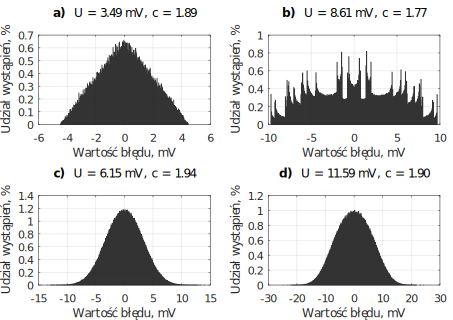
\includegraphics{obrazki/hist_part_a}
\makecaption{fig:symul_parta_hist}{Histogramy realizacji sygnałów błędów \textbf{a)}~statycznego, \textbf{b)}~dynamicznego, \textbf{c)}~losowego, \textbf{d)}~wypadkowego, wielkości wyjściowej analizowanego w eksperymencie symulacyjnym przetwornika pomiarowego uzyskane metodą Monte-Carlo}
\end{center}
\end{figure}

Wyznaczona na drodze eksperymentu wartość wielkości $U_{a,\Sigma}$ wyniosła~\qty{11.58}{mV}, przy czym wartość współczynnika rozszerzenia $c_{a,\Sigma}$ wyniosła~\num{1.90}. Wartość niepewności oszacowana na podstawie równania~\eqref{eq:sym_parta_uncert_value_a} jest zatem około~\qty{4.5}{\percent} większa od wartości uzyskanej na drodze eksperymentu. Należy zaznaczyć, że ta sama wartość wyznaczona za pomocą równania~\eqref{eq:sym_parta_uncert_sum} stosując współczynniki koherencji, których wartości zostały wyznaczone bez użycia zaproponowanej w pracy korekty opisanej równaniem~\eqref{eq:unc_cohercorra} wynosi~\qty{12.41}{mV}, a zatem jest ona o~\qty{7.3}{\percent} większa od wartości referencyjnej. W przypadku wartości oszacowanej na podstawie równania~\eqref{eq:sym_parta_uncert_value_b} rozbieżność jest nieco mniejsza i wynosi około~\qty{3.2}{\percent}, co dowodzi że w analizowanym przypadku spełnione zostały założenia związane z centralnym twierdzeniem granicznym, a przyjęte uproszczenia okazały się nie mieć znaczącego wpływu na wynik obliczeń. Uzyskana wartość wariancji sygnału błędu wypadkowego wielkości wyjściowej wyniosła w eksperymencie~\qty{37.1}{\micro V}, co pokrywa się z wartością wyznaczoną w równaniu~\eqref{eq:sym_parta_var_sum}. Wyznaczone w równaniach od~\eqref{eq:sym_parta_uncert_stat} do~\eqref{eq:sym_parta_factor_rand} parametry dla składowych sygnału błędu również w zadowalającym stopniu pokrywają się z uzyskanymi na drodze eksperymentu.

Zastosowana metoda szacowania wartości współczynników koherencji w celu wyznaczenia wypadkowej wartości niepewności rozszerzonej zapewnia wyniki zawyżone o kilka procent w stosunku do wartości uzyskiwanych symulacyjne. Jako, że omawiane rozbieżności są niewielkie oraz ich znak jest dodatni, uzyskiwane wyniki można uznać za prawidłowe. Wadą przedstawionej metody jest jednak konieczność znajomości wartości współczynników kształtu, co powoduje, że dla rozkładów o niestandardowym kształcie jej obszar zastosowań staje się ograniczony. Zaproponowana w pracy dodatkowa korekta wartości współczynników koherencji pozwala na uzyskanie bardziej zbliżonych, do uzyskiwanych symulacyjnie, wyników obliczeń.

Wobec przedstawionych rozważań i wyników przeprowadzonego eksperymentu stwierdzić można, że zaproponowany model błędu odpowiednio opisuje związki pomiędzy kolejnymi sygnałami błędów, zachodzące w analizowanym obiekcie. Jako, że kolejne fragmenty analizowanego toru pomiarowego przetwarzać będą zdefiniowane dotychczas sygnały błędów, przeprowadzony proces wyznaczania parametrów wypadkowych w przypadku grupy błędów dynamicznych oraz wyznaczanie parametrów wypadkowego błędu wielkości wyjściowej był bezzasadny i został przeprowadzony jedynie w celu weryfikacji zaproponowanej metody obliczeń. W przypadku pozostałych grup sygnałów błędów, które cechowały się rozkładami o standardowych kształtach, wyznaczenie wypadkowych parametrów tych sygnałów pozwala na zmniejszenie liczby analizowanych sygnałów i upraszcza dalszą analizę.

\section{Analiza wzmacniacza pomiarowego}

Kolejną część toru pomiarowego stanowi wzmacniacz, którego zadaniem jest dopasowanie poziomu sygnału napięciowego $y_{a}(t)$, reprezentującego mierzoną wielkość fizyczną $s(t)$, do zakresu napięcia wejściowego $y_{b}(t)$ przetwornika analogowo-cyfrowego. Zakładane wzmocnienie układu wynosi $s_{b} = \qty{3.3}{V \per V}$, zatem w przypadku idealnym jego funkcję przetwarzania $\dot{f}_{b}(x)$ stanowi addytywna funkcja liniowa opisana równaniem:
\begin{equation}
\dot{f}_{b} \emb{x} = s_{b} x = \num{3.3} x \label{eq:sym_partb_function},
\end{equation}
przy czym przyjmuje się, że nieliniowość przedstawionej charakterystyki jest pomijalnie mała i nie została rozważona w przedstawionym eksperymencie, a zatem przyjąć można założenie, gdzie $\tilde{f}_{b}(x) \cong \dot{f}_{b}(x)$. Wobec powyższych wielkość wyjściową analizowanego obiektu opisać można jako:
\begin{gather}
\dot{y}_{b} \emb{t} = \dot{f}_{b} \emb{\dot{y}_{a} \emb{t}} = \num{3.3} \dot{y}_{a} \emb{t} \label{eq:sym_partb_out_ideal}, \\
\tilde{y}_{b} \emb{t} = \dot{y}_{b} \emb{t} + e_{b,\Sigma} \emb{t} \label{eq:sym_partb_out_real},
\end{gather}
gdzie sygnały wchodzące w skład wypadkowego sygnału błędu $e_{b,\Sigma}(t)$ opisano w dalszej części podrozdziału oraz wskazano ich parametry.

Analizowany układ wzmacniacza charakteryzuje się częstotliwością graniczną równą $f_{b,g} = \qty{650}{kHz}$, stąd zakłada się, że jego transmitancje opisać można w postaci:
\begin{equation}
\tilde{G}_{b} \emb{j\omega} = \frac{1}{1 + j \frac{\omega}{2 \pi f_{b,g}}} = \frac{1}{\frac{\omega^{2}}{4 \pi^{2} f_{b,g}^{2}} + 1} - j \frac{\omega}{2 \pi f_{b,g} \left( \frac{\omega^{2}}{4 \pi^{2} f_{b,g}^{2}} + 1 \right) } \label{eq:sym_partb_trans}.
\end{equation}
Wobec przedstawionego założenia, równania~\eqref{eq:mid_cont_amp} oraz~\eqref{eq:mid_cont_phi} można rozwinąć jako:
\begin{gather}
\tilde{K}_{b} \emb{\omega} = \sqrt{\left( \Re \left( \tilde{G}_{b} \emb{j\omega} \right) \right)^{2} + \left( \Im \left( \tilde{G}_{b} \emb{j\omega} \right) \right)^{2}} = \left( \frac{\omega^{2}}{4 \pi^{2} f_{b,g}^{2}} + 1 \right)^{-\frac{1}{2}} \label{eq:sym_partb_amp_real}, \\
\tilde{\varphi}_{b} \emb{\omega} = \arctan \left( \frac{\Im \left( \tilde{G}_{b} \emb{j\omega} \right)}{\Re \left( \tilde{G}_{b} \emb{j\omega} \right)} \right) = \arctan \left( -\frac{\omega}{2 \pi f_{b,g}} \right) \label{eq:sym_partb_phi_real},
\end{gather}
natomiast w przypadku idealnej transmitancji $\dot{G}_{b}(j\omega) = 1$, parametry te wynoszą kolejno:
\begin{gather}
\dot{K}_{b} \emb{\omega} = \sqrt{\left( \Re \left( \dot{G}_{b} \emb{j\omega} \right) \right)^{2} + \left( \Im \left( \dot{G}_{b} \emb{j\omega} \right) \right)^{2}} = 1 \label{eq:sym_partb_amp_ideal}, \\
\dot{\varphi}_{b} \emb{\omega} = \arctan \left( \frac{\Im \left( \dot{G}_{b} \emb{j\omega} \right)}{\Re \left( \dot{G}_{b} \emb{j\omega} \right)} \right) = 0 \label{eq:sym_partb_phi_ideal}.
\end{gather}

Wobec przyjętych dotychczas założeń, opisanych w równaniach~\eqref{eq:sym_partb_out_ideal}, \eqref{eq:sym_partb_amp_ideal}, \eqref{eq:sym_partb_phi_ideal} oraz założenia określającego idealny przebieg przetwarzanej wielkości wejściowej $y_{a}(t)$, opisanego równaniem~\eqref{eq:sym_parta_out_ideal_sum}, idealny przebieg wielkości wyjściowej $y_{b}(t)$ w analizowanym przypadku określa równanie:
\begin{equation}
\dot{y}_{b} \emb{t} = \sum _{i=1} ^{3} E_{b,o} \emb{\omega_{b,i}} \sin \emb{\omega_{b,i} t + \varphi_{b,i}} \label{eq:sym_partb_out_ideal_sum},
\end{equation}
natomiast parametry kolejnych harmonicznych przedstawionego sygnału opisać można dla przypadku idealnego, jako:
\begin{gather}
E_{b,o} \emb{\omega} = \dot{f}_{b} \emb{\dot{K}_{b} \emb{\omega} E_{a,o} \emb{\omega}} = \num{3.3} E_{a,o} \emb{\omega} \label{eq:sym_partb_amp_out_ideal}, \\
\varphi_{b,o} \emb{\omega} = \varphi_{a,o} \emb{\omega} + \dot{\varphi}_{b} \emb{\omega} = \varphi_{a,o} \emb{\omega} \label{eq:sym_partb_phi_out_ideal},
\end{gather}
gdzie $E_{b,o}(\omega)$ jest amplitudą oraz $\varphi_{b,o}(\omega)$ fazą harmonicznej sygnału wyjściowego $y_{a}(t)$ o wybranej pulsacji w przypadku idealnym, natomiast $\omega_{a,i} = \omega_{b,i}$ jest pulsacją $i$-tej harmonicznej analizowanego sygnału. Na podstawie danych zestawionych w tabeli~\ref{tab:sym_outa_params_ideal} oraz zależności od~\eqref{eq:sym_partb_out_ideal_sum} do~\eqref{eq:sym_partb_phi_out_ideal} wyznaczono parametry sygnału $y_{b}(t)$ dla przypadku idealnego i zestawiono je w tabeli~\ref{tab:sym_outb_params_ideal}.

\begin{table}[htb!]
\begin{center}
\makecaption{tab:sym_outb_params_ideal}{Parametry kolejnych harmonicznych sygnału $y_{b}(t)$ przyjęte w przeprowadzanym eksperymencie symulacyjnym dla sytuacji idealnej}
\begin{tabular}[c]{| c | c | c | c |} \hline
\textbf{Lp. $i$} & \textbf{Pulsacja $\omega_{a,i}$, rad/s} & \textbf{Amplituda $E_{a,o}(\omega_{a,i})$, V} & \textbf{Faza $\varphi_{a,o}(\omega_{a,i})$, rad} \\ \hline
1 & $1000  \cdot 2\pi$ &  \num{0.6} & $0$           \\ \hline
2 & $5000  \cdot 2\pi$ &  \num{0.3} & $\pi/8 + \pi$ \\ \hline
3 & $15000 \cdot 2\pi$ &  \num{0.1} & $\pi/6$       \\ \hline
\end{tabular}
\end{center}
\end{table}

Pierwszą omawianą grupę sygnałów błędów stanowią błędy własne, wprowadzane przez analizowany obiekt. Przyjmuje się, że temperatura otoczenia $\vartheta(t)$ wpływa na dryf zera analizowanego wzmacniacza zgodnie z zależnością opisaną równaniem:
\begin{equation}
f_{b,z} \left( \vartheta \emb{t} \right) = \frac{7}{2} \left( \vartheta \emb{t} - \qty{20}{\degreeCelsius} \right)~\unit{\frac{mV}{K}} \label{eq:sym_partb_temp_err},
\end{equation}
oraz że w czasie wykonywania pojedynczej serii pomiarowej zmiany tej temperatury będą zbliżone do zera. Błąd statyczny własny, wynikający z dryfu zera spowodowanego zmianą temperatury otoczenia, zgodnie z równaniem~\eqref{eq:out_cont_err_env_self} opisać można jako:
\begin{equation}
e_{b,sw} \emb{t} = f_{b,z} \left( \vartheta \emb{t} \right) \label{eq:sym_partb_err_sw}.
\end{equation}
Sygnał błędu dynamicznego własnego, zdefiniowany w równaniach~\eqref{eq:mid_cont_err_dyn_prop} oraz~\eqref{eq:out_cont_err_dyn_prop}, opisać można na podstawie założeń danych równaniem~\eqref{eq:sym_parta_out_ideal_sum} w postaci:
\begin{equation}
e_{b,dw} \emb{t} = \sum _{i = j} ^{3} e_{b,dw} \emb{t,\omega_{a,j}} = \sum _{i = j} ^{3} E_{b,ew} \emb{\omega_{b,j}} \sin \emb{\omega t + \varphi_{b,ew} \emb{\omega_{b,j}}} \label{eq:sym_partb_dyn_self_sum},
\end{equation}
natomiast kolejne harmoniczne przedstawionego sygnału mogą być opisane następująco:
\begin{equation}
\begin{split}
e_{b,dw} \emb{t,\omega} =~
& \tilde{f}_{b} \left( \tilde{K}_{b} \emb{\omega} E_{a,o} \emb{\omega} \sin \left( \omega t + \varphi_{a,o} \emb{\omega} + \tilde{\varphi}_{b} \emb{\omega} \right) \right)- \\
& \tilde{f}_{b} \left( \dot{K}_{b} \emb{\omega} E_{a,o} \emb{\omega} \sin \left( \omega t + \varphi_{a,o} \emb{\omega} + \dot{\varphi}_{b} \emb{\omega} \right) \right)
\end{split}
\label{eq:sym_partb_dyn_self_err}.
\end{equation}
Parametry składowych przetwarzanego sygnału $y_{a}(t)$ w funkcji pulsacji dla przypadku idealnego zdefiniowano w równaniach~\eqref{eq:sym_parta_amp_out_ideal} oraz~\eqref{eq:sym_parta_phi_out_ideal}, natomiast w tabeli~\ref{tab:sym_outb_params_ideal} zestawiono wyznaczone wartości tych parametrów dla przyjętych odnośnie przetwarzanego sygnału $s(t)$ założeń, danych równaniem~\eqref{eq:sym_in_ideal} i podsumowanych w tabeli~\ref{tab:sym_in_params_ideal}.

Drugą grupę sygnałów błędów stanowią błędy propagowane, przenoszone z wejścia na wyjście obiektu. Sygnał błędu statycznego $e_{a,sw}(t)$ jest przenoszony na wyjście obiektu zgodnie równaniami~\eqref{eq:mid_cont_err_stat_prop} oraz~\eqref{eq:out_cont_err_stat_prop}, zatem:
\begin{equation}
e_{b,sp} \emb{t} = \tilde{f}_{b} \left( \tilde{K}_{b} \emb{0} e_{a,sw} \emb{t} \right) = \num{3.3} e_{a,sw} \emb{t} \label{eq:sym_partb_stat_prop_err},
\end{equation}
Sygnały błędów losowych $e_{a,rw}(t)$ oraz $e_{a,rp}(t)$ wielkości wejściowej są propagowane zgodnie z zależnością~\eqref{eq:out_cont_err_rand_prop}, przy czym ze względu na niedeterministyczny opis tych sygnałów nie ma możliwości zdefiniowania postaci tych sygnałów w funkcji czasu. Stosując zaproponowany model błędu należy jedynie zdefiniować parametry tych sygnałów na wyjściu obiektu, zatem przyjmuje się, że sygnał błędu $e_{b,rp,1}(t)$ na wyjściu obiektu związany jest z sygnałem $e_{a,rw}(t)$ na jego wejściu, oraz że sygnał $e_{b,rp,2}(t)$ na wyjściu obiektu jest powiązany z sygnałem $e_{a,rp}(t)$. Na podstawie wprowadzonych założeń wypadkowy sygnał propagowanego błędu losowego wyrazić można w postaci:
\begin{equation}
e_{b,rp} \emb{t} = e_{b,rp,1} \emb{t} + e_{b,rp,2} \emb{t} \label{eq:sym_partb_rand_prop_err},
\end{equation}
Przetwarzany przez obiekt sygnał błędu dynamicznego $e_{a,dw}(t)$ propagowany jest na wyjście zgodnie z równaniami~\eqref{eq:mid_cont_err_dyn_prop} oraz~\eqref{eq:out_cont_err_dyn_prop}, zatem wybraną harmoniczną sygnału propagowanego błędu dynamicznego $e_{b,dp}(t)$ na wyjściu tego obiektu opisuje równanie:
\begin{equation}
\begin{split}
e_{b,dp} \emb{t,\omega} =~
& \dot{f}_{b} \left( \tilde{K}_{b} \emb{\omega} E_{a,e} \emb{\omega} \sin \left( \omega t + \varphi_{a,e} \emb{\omega} + \tilde{\varphi}_{b} \emb{\omega} \right) \right) = \\
& \num{3.3} \tilde{K}_{b} \emb{\omega} E_{a,e} \emb{\omega} \sin \left( \omega t + \varphi_{a,e} \emb{\omega} + \tilde{\varphi}_{b} \emb{\omega} \right)
\end{split}
\label{eq:sym_partb_dyn_prop_err},
\end{equation}
natomiast wypadkowe parametry kolejnych harmonicznych przetwarzanego sygnału błędu dynamicznego $e_{a,dw}(t)$ zestawiono w tabeli~\ref{tab:sym_parta_params_dyn_summary}. Wypadkowy sygnał błędu dynamicznego propagowanego zdefiniować można zatem jako:
\begin{equation}
e_{b,dp} \emb{t} = \sum _{j = 1} ^{3} e_{b,dp} \emb{t,\omega_{a,j}} = \sum _{i = j} ^{3} E_{b,ep} \emb{\omega_{b,j}} \sin \emb{\omega t + \varphi_{b,ep} \emb{\omega_{b,j}}} \label{eq:sym_partb_dyn_prop_sum},
\end{equation}
przy czym omówiony przypadek dotyczy założeń przyjętych w równaniu~\eqref{eq:sym_parta_dyn_self_sum}, które wynikają z założonej w równaniu~\eqref{eq:sym_in_ideal} postaci sygnału $s(t)$.

Parametry wypadkowe kolejnych harmonicznych sygnałów błędów dynamicznych własnych $e_{b,dw}(t)$ oraz propagowanych $e_{b,dp}(t)$ mogą być wyznaczone w sposób analogiczny, jak pokazano na przykładnie opisanym w równaniach od~\eqref{eq:sym_parta_dyn_self_example_sum} do~\eqref{eq:sym_parta_dyn_self_example_phi}. Wyznaczenie omawianych parametrów pozwoli na określenie wartości wariancji wymienionych sygnałów oraz wyznaczenie związanej z nimi wartości niepewności rozszerzonej. Wyznaczone zgodnie z metodą zaproponowaną w równaniach od~\eqref{eq:dyn_vect} do~\eqref{eq:dyn_vect_phi} wypadkowe amplitudy oraz fazy dla wskazanych sygnałów błędów dynamicznych przedstawiono w tabelach~\ref{tab:sym_partb_params_dyn_self} oraz~\ref{tab:sym_partb_params_dyn_prop}. Należy zauważyć, wyznaczenie wypadkowych parametrów kolejnych harmonicznych analizowanych sygnałów nie jest konieczne z punktu widzenia stosowania zaproponowanego modelu błędu. Zabieg ten pozwala natomiast uprościć analizę poprzez redukcję liczby analizowanych sygnałów.

\begin{table}[htb!]
\begin{center}
\makecaption{tab:sym_partb_params_dyn_self}{Parametry wypadkowe kolejnych harmonicznych sygnału błędu dynamicznego własnego analizowanego w eksperymencie symulacyjnym wzmacniacza pomiarowego}
\begin{tabular}[c]{| c | c | S[table-format = 2.2] | S[table-format = +1.2] |} \hline
\textbf{Lp. $j$} & \textbf{Pulsacja $\omega_{b,j}$, rad/s} & \textbf{Amplituda $E_{b,e}(\omega_{b,j})$, mV} & \textbf{Faza $\varphi_{b,e}(\omega_{b,j})$, rad} \\ \hline
1 & $1000  \cdot 2\pi$  &   9.23  & -1.57  \\ \hline
2 & $5000  \cdot 2\pi$  &  23.08  &  1.96  \\ \hline
3 & $15000 \cdot 2\pi$  &  23.07  & -1.07  \\ \hline
\end{tabular}
\end{center}
\end{table}

\begin{table}[htb!]
\begin{center}
\makecaption{tab:sym_partb_params_dyn_prop}{Parametry wypadkowe kolejnych harmonicznych sygnału błędu dynamicznego propagowanego analizowanego w eksperymencie symulacyjnym wzmacniacza pomiarowego}
\begin{tabular}[c]{| c | c | S[table-format = 2.2] | S[table-format = +1.2] |} \hline
\textbf{Lp. $j$} & \textbf{Pulsacja $\omega_{b,j}$, rad/s} & \textbf{Amplituda $E_{b,e}(\omega_{b,j})$, mV} & \textbf{Faza $\varphi_{b,e}(\omega_{b,j})$, rad} \\ \hline
1 & $1000  \cdot 2\pi$  &   9.23  & -1.57  \\ \hline
2 & $5000  \cdot 2\pi$  &  23.08  &  1.96  \\ \hline
3 & $15000 \cdot 2\pi$  &  23.07  & -1.07  \\ \hline
\end{tabular}
\end{center}
\end{table}

Cel następnego etapu rozważań stanowi określenie parametrów wariancji oraz niepewności rozszerzonych dla opisanych dotychczas sygnałów błędów. Ze względu na liniowy charakter analizowanego obiektu, wynikający z przyjętych założeń, opisanych w równaniach~\eqref{eq:sym_partb_out_ideal} oraz~\eqref{eq:sym_partb_trans}, na wyjściu obiektu zachowane zostaną oryginalne kształty rozkładów wszystkich propagowanych sygnałów błędów~\cite{grimmett_probability}. Wobec powyższych, znając wariancję tych sygnałów na wyjściu obiektu, wyznaczenie związanej z nimi wartości niepewności rozszerzonej odbywać się może zgodnie z zależnością~\eqref{eq:unc_sum}. Wpływ transmitancji obiektu na wartość wariancji propagowanych sygnałów błędów opisany został wcześniej równaniem~\eqref{eq:mid_cont_var_omega}, natomiast wpływ funkcji przetwarzania na tą wielkość w przypadku liniowej funkcji przetwarzania określa zależność~\eqref{eq:out_cont_var_sense}. Można zatem zapisać, w przypadku sygnału propagowanego błędu statycznego:
\begin{gather}
\sigma_{b,sp}^{2} = s_{b}^{2} \tilde{K}_{b}^{2} \emb{0} \sigma_{a,sw}^{2} = \num{3.3}^{2} \cdot \num{1.0}^{2} \cdot \num{3.38} = \qty{36.75}{\micro V} \label{eq:sym_partb_var_stat_prop}, \\
U_{b,sp} = c_{b,sp} \sigma_{b,sp} = \qty{11.52}{mV} \label{eq:sym_partb_unc_stat_prop},
\end{gather}
gdzie $c_{b,sp} = c_{a,sw} = c_{t} = \num{1.90}$. W przypadku kolejnych harmonicznych sygnału błędu dynamicznego, ich wariancję opisać można zgodnie z zależnością~\eqref{eq:dyn_var} na podstawie wypadkowych parametrów tych harmonicznych, zestawionych w tabelach~\ref{tab:sym_partb_params_dyn_self} oraz~\ref{tab:sym_partb_params_dyn_prop}. Wariancję sygnałów błędów losowych $e_{b,rp,1}(t)$ oraz $e_{b,rp,2}(t)$ można natomiast opisać w funkcji pulsacji, jako:
\begin{gather}
\sigma_{b,rp,1}^{2} \emb{\omega} = s_{b}^{2} \tilde{K}_{b} \emb{\omega} \sigma_{a,rw}^{2} \emb{\omega} \cong \qty{36.26}{\micro V} \label{eq:sym_partb_var_rand_prop_1}, \\
\sigma_{b,rp,2}^{2} \emb{\omega} = s_{b}^{2} \tilde{K}_{b} \emb{\omega} \sigma_{a,rp}^{2} \emb{\omega} = s_{a}^{2} s_{b}^{2} \tilde{K}_{a}^{2} \emb{\omega} \tilde{K}_{b} \emb{\omega} \sigma_{s,r}^{2} \emb{\omega} \cong \qty{72.64}{\micro V} \label{eq:sym_partb_var_rand_prop_2},
\end{gather}
przy czym postać przedstawionych zależności wynika z faktu, że w zakresie częstotliwości $\hat{f} \in~<0;\frac{1}{2} f_{p}>$ transmitancja obiektu nie wpływa na widmo przetwarzanych sygnałów błędów losowych. Można zatem, zgodnie z zależnością~\eqref{eq:out_cont_err_rand_prop}, przyjąć założenia gdzie $e_{b,rp,1}(t) = \tilde{f}_{b}(e_{a,rw}(t))$ oraz $e_{b,rp,2}(t) = \tilde{f}_{b}(e_{a,rp}(t))$. Wartości niepewności rozszerzonych związanych z analizowanymi sygnałami opisują zatem równania:
\begin{gather}
U_{b,rp,1} = c_{b,rp,1} \sigma_{b,rp,1} = \qty{9.93}{mV} \label{eq:sym_partb_uncert_rand_prop_1}, \\
U_{b,rp,2} = c_{b,rp,2} \sigma_{b,rp,2} = \qty{16.70}{mV} \label{eq:sym_partb_uncert_rand_prop_2},
\end{gather}
gdzie $c_{b,rp,1} = c_{a,rw} = c_{u} = \num{1.65}$ oraz $c_{b,rp,2} = c_{a,rp} = c_{n} = \num{1.96}$. Należy zauważyć, że w przypadku istnienia wpływu transmitancji obiektu na widmową gęstość mocy analizowanych sygnałów, w celu wyznaczenia wartości niepewności rozszerzonej związanej z tymi sygnałami należałoby określić średnią wartość wariancji tych sygnałów dla analizowanego zakresu częstotliwości, określoną równaniem~\eqref{eq:mid_cont_var_rand}. Tabela~\ref{tab:sym_partb_params_unc_list} przedstawia budżet niepewności wielkości wyjściowej analizowanego wzmacniacza pomiarowego z uwzględnieniem podziału na sygnały błędów własnych i propagowanych, sporządzony na podstawie przedstawionych rozważań.

\begin{table}[htb!]
\begin{center}
\makecaption{tab:sym_partb_params_unc_list}{Budżet niepewności wielkości wyjściowej analizowanego w eksperymencie symulacyjnym wzmacniacza pomiarowego, gdzie (a)~oznacza przetwornik pomiarowy oraz (b)~oznacza wzmacniacz pomiarowy}
\begin{tabular}[c]{| c | c | S[table-format = 2.2] | S[table-format = 3.2] | c | c |} \hline
\textbf{Lp.} & \textbf{Symbol} & \textbf{$U$, mV} & \textbf{$\sigma^{2}$, \micro V} & \textbf{Rozkład} & \textbf{Źródło błędu} \\ \hline
1  & ${b,sp}$       & 11.52 &  36.75  & trójkątny                    & dryf temperatury (a)                       \\ \hline
2  & ${b,sw}$       & 8.15  &  18.38  & trójkątny                    & dryf temperatury (b)                       \\ \hline
3  & ${b,rp,1}$     & 9.93  &  36.26  & jednostajny                  & nieliniowość obiektu (a)                   \\ \hline
4  & ${b,rp,2}$     & 16.70 &  72.64  & normalny                     & szum wielkości wejściowej                  \\ \hline
5  & ${b,dp,1}$     & 6.21  &  19.14  & \multirow{6}{*}{dwumodalny}  & \multirow{3}{*}{transmitancja (a)}         \\ \cline{1-4}
6  & ${b,dp,2}$     & 15.53 &  119.62 &                              &                                            \\ \cline{1-4}
7  & ${b,dp,3}$     & 15.52 &  119.44 &                              &                                            \\ \cline{1-4} \cline{6-6}
8  & ${b,dw,1}$     & 3.06  &  4.64   &                              & \multirow{3}{*}{transmitancja (b)}         \\ \cline{1-4}
9  & ${b,dw,2}$     & 7.65  &  29.00  &                              &                                            \\ \cline{1-4}
10 & ${b,dw,3}$     & 7.65  &  28.99  &                              &                                            \\ \hline
\end{tabular}
\end{center}
\end{table}

Dla źródeł błędów wymienionych w budżecie niepewności, zestawionym w tabeli~\ref{tab:sym_partb_params_unc_list}, konieczne jest określenie wzajemnych korelacji pomiędzy sygnałami błędów. Należy zauważyć, że składowe związane z dryfem temperaturowym przetwornika pomiarowego oraz dryfem temperaturowym wzmacniacza zależą od tej samej wielkości fizycznej -- temperatury otoczenia. Jako, że wymienione sygnały błędów nie zależą od żadnej innej wielkości, a dodatkowo równania~\eqref{eq:sym_parta_stat_err} oraz~\eqref{eq:sym_partb_temp_err} cechują się dodatnią czułością względem tej wielkości, można założyć pełną dodatnią korelacje analizowanych sygnałów błędów, zatem $r_{b,sw,b,sp} = r_{b,sp,b,sw} = 1$. W przypadku kolejnych harmonicznych sygnałów błędów dynamicznych wartość współczynnika korelacji tych składowych może być obliczona zgodnie z równaniem~\eqref{eq:dyn_corr}. Można zauważyć, że wartość tego współczynnika dla par składowych o różnej pulsacji każdorazowo wyniesie zero. W przypadku par harmonicznych sygnałów błędów dynamicznych o identycznej pulsacji, na podstawie danych zawartych w tabelach~\ref{tab:sym_partb_params_dyn_self} oraz~\ref{tab:sym_partb_params_dyn_prop}, zauważyć można, że współczynnik korelacji zbliżony będzie od jedności, ze względu na zbliżoną do zera różnicę w fazach tych sygnałów. W przypadku pozostałych par sygnałów wartości współczynników korelacji będą zerowe.

Biorąc pod uwagę przedstawione informacje na temat istniejących korelacji pomiędzy analizowanymi sygnałami błędów należy zauważyć, że zastosowanie opisanej równaniem~\eqref{eq:unc_matrix} metody wyznaczania wypadkowej wartości niepewności rozszerzonej nie będzie możliwe dla wartości współczynników koherencji wyznaczanych zgodnie z równaniem~\eqref{eq:unc_coher}. Ograniczenie to wynika z faktu, że opisane w równaniach~\eqref{eq:unc_cohercorra} oraz~\eqref{eq:unc_cohercorrb} korekty nie są odpowiednie dla sytuacji, gdzie pomiędzy analizowanymi sygnałami występuje korelacja. Proponuje się zatem, w celu umożliwienia zastosowania przedstawionej metody analizy, wyznaczenie wypadkowych parametrów wariancji i niepewności rozszerzonych dla skorelowanych grup sygnałów. Jako, że zaproponowana operacja prowadzi do redukcji liczby analizowanych sygnałów błędów poprzez wprowadzenie wypadkowych sygnałów dla analizowanych grup, proponuje się równolegle określić budżet niepewności dla rozważanego fragmentu toru pomiarowego, który zorientowany będzie pod kątem charakteru realizacji wymienionych w nim sygnałów.

Na podstawie zależności od~\eqref{eq:sym_partb_err_sw} do~\eqref{eq:sym_partb_dyn_prop_sum}, zgodnie z równaniem~\eqref{eq:out_cont_err_sum_all}, opisać można wprowadzony w równaniu~\eqref{eq:sym_partb_out_real} wypadkowy sygnał błędu $e_{b,\Sigma}(t)$ wielkości wyjściowej analizowanego wzmacniacza pomiarowego następującym równaniem:
\begin{equation}
e_{b,\Sigma} \emb{t} = e_{b,s} \emb{t} + e_{b,d} \emb{t} + e_{b,s} \emb{t} \label{eq:sym_partb_error_sum},
\end{equation}
w którym kolejne składniki przedstawionego sygnału zdefiniowane są w postaci:
\begin{gather}
e_{b,s} \emb{t} = e_{b,sw} \emb{t} + e_{b,sp} \emb{t} \label{eq:sym_partb_error_stat}, \\
e_{b,d} \emb{t} = e_{b,dw} \emb{t} + e_{b,dp} \emb{t} \label{eq:sym_partb_error_dyn}, \\
e_{b,r} \emb{t} = e_{b,rp} \emb{t} \label{eq:sym_partb_error_rand},
\end{gather}
gdzie $e_{b,s}(t)$ jest wypadkowym sygnałem błędu statycznego, $e_{b,d}(t)$ dynamicznego oraz $e_{b,r}(t)$ losowego. Wypadkowy sygnał błędu dynamicznego opisać można w postaci:
\begin{equation}
e_{b,d} \emb{t} = \sum _{k=1} ^{3} E_{b,e} \emb{\omega_{b,k}} \sin \emb{\omega t + \varphi_{b,e} \emb{\omega_{b,k}}} \label{sym_partb_error_dyn_sum},
\end{equation}
przy czym $E_{b,e}(\omega)$ jest wypadkową amplitudą, natomiast $\varphi_{b,e}(\omega)$ wypadkową fazą harmonicznej tego sygnału o wskazanej pulsacji. Wyznaczenie wypadkowych wartości amplitudy oraz fazy dla kolejnych harmonicznych sygnału błędu dynamicznego $e_{b,d}(t)$ przebiega zgodnie z metodą zaproponowaną w równaniach od~\eqref{eq:dyn_vect} do~\eqref{eq:dyn_vect_phi}, przy czym kolejne składniki tych harmonicznych wymienione są w równaniach~\eqref{eq:sym_partb_dyn_self_err} oraz~\eqref{eq:sym_partb_dyn_prop_err}. Przedstawiony proces odbywać się może również z wykorzystaniem parametrów opisanych w tabelach~\ref{tab:sym_partb_params_dyn_self} oraz~\ref{tab:sym_partb_params_dyn_prop}, przy czym niezależnie od stosowanej metody uzyskuje się identyczne wyniki obliczeń. Wartości omawianych parametrów wyznaczone zgodnie z przedstawionymi zależnościami zestawiono w tabeli~\ref{tab:sym_partb_params_dyn_summary}.

\begin{table}[htb!]
\begin{center}
\makecaption{tab:sym_partb_params_dyn_summary}{Parametry wypadkowe kolejnych harmonicznych sygnału błędu dynamicznego analizowanego w eksperymencie symulacyjnym wzmacniacza pomiarowego}
\begin{tabular}[c]{| c | c | S[table-format = 2.2] | S[table-format = +1.2] |} \hline
\textbf{Lp. $k$} & \textbf{Pulsacja $\omega_{b,k}$, rad/s} & \textbf{Amplituda $E_{b,e}(\omega_{b,k})$, mV} & \textbf{Faza $\varphi_{b,e}(\omega_{b,k})$, rad} \\ \hline
1 & $1000  \cdot 2\pi$  &   9.23  & -1.57  \\ \hline
2 & $5000  \cdot 2\pi$  &  23.08  &  1.96  \\ \hline
3 & $15000 \cdot 2\pi$  &  23.07  & -1.07  \\ \hline
\end{tabular}
\end{center}
\end{table}

Parametry wypadkowego błędu statycznego, danego zależnością~\eqref{eq:sym_partb_error_stat}, opisują równania~\eqref{eq:var_matrix} oraz~\eqref{eq:unc_matrix}, przy czym w bieżącym przypadku przyjmują one postać:
\begin{gather}
\begin{split}
\sigma_{b,s}^{2} = ~ &
\begin{bmatrix}
\sigma_{b,sw} \\ \sigma_{b,sp}
\end{bmatrix}^{T}
\begin{bmatrix}
1 & r_{b,sw,sp} \\
r_{b,sp,rw} & 1
\end{bmatrix}
\begin{bmatrix}
\sigma_{b,sw} \\ \sigma_{b,sp}
\end{bmatrix} = \\ &
\begin{bmatrix}
\num{6.06e-3} \\ \num{4.29e-3}
\end{bmatrix}^{T}
\begin{bmatrix}
1 & 1 \\
1 & 1
\end{bmatrix}
\begin{bmatrix}
\num{6.06e-3} \\ \num{4.29e-3}
\end{bmatrix} = \qty{107.12}{\micro V}
\end{split}
\label{eq:sym_partb_stat_var}. \\
\begin{split}
U_{b,s} = ~ & \sqrt{
\begin{bmatrix}
U_{b,sw} \\ U_{b,sp}
\end{bmatrix}^{T}
\begin{bmatrix}
1 & h_{b,sw,sp} \\
h_{b,sp,rw} & 1
\end{bmatrix}
\begin{bmatrix}
U_{b,sw} \\ U_{b,sp}
\end{bmatrix}} = \\ & \sqrt{
\begin{bmatrix}
\num{11.52e-3} \\ \num{8.15e-3}
\end{bmatrix}^{T}
\begin{bmatrix}
1 & 1 \\
1 & 1
\end{bmatrix}
\begin{bmatrix}
\num{11.52e-3} \\ \num{8.15e-3}
\end{bmatrix}} = \qty{19.67}{mV}
\end{split}
\label{eq:sym_partb_stat_uncert},
\end{gather}
gdzie współczynniki koherencji $h_{b,sw,sp} = h_{b,sp,sw} = 1$ w przypadku pełnej dodatniej korelacji, jaka ma miejsce w omawianym przypadku. W przypadku sygnałów błędów losowych propagowanych korelacja nie występuje, a zatem wariancja wypadkowego sygnału błędu losowego jest wyznaczana zgodnie z zależnością~\eqref{eq:var_sum} jako:
\begin{equation}
\sigma_{b,r}^{2} = \sigma_{b,rp,1}^{2} + \sigma_{b,rp,2}^{2} = \qty{108.90}{\micro V} \label{eq:sym_partb_rand_var}.
\end{equation}
Wypadkową niepewność rozszerzoną w analizowanym przypadku wyznaczyć można zgodnie z równaniem~\eqref{eq:unc_sum}, przy czym:
\begin{gather}
\begin{split}
U_{a,r} = ~ & \sqrt{
\begin{bmatrix}
U_{a,rp,1} \\ U_{b,rp,2}
\end{bmatrix}^{T}
\begin{bmatrix}
1            & h_{a,rp,1,2} \\
h_{a,rp,2,1} & 1
\end{bmatrix}
\begin{bmatrix}
U_{a,rp,1} \\ U_{b,rp,2}
\end{bmatrix}} = ~ \\ & \sqrt{
\begin{bmatrix}
\num{9.93e-3} \\ \num{16.70e-3}
\end{bmatrix}^{T}
\begin{bmatrix}
\num{1.000} & \num{0.120} \\
\num{0.120} & \num{1.000}
\end{bmatrix}
\begin{bmatrix}
\num{9.93e-3} \\ \num{16.70e-3}
\end{bmatrix}} = \qty{20.43}{mV}
\end{split}
\label{eq:sym_partb_rand_uncert}, \\
h_{b,rp,1,2} = s_{u,n} \sqrt{\frac{\num{9.93e-3}}{\num{16.70e-3}}} \left( \frac{\num{98.60e-6} + \num{278.89e-6}}{\num{377.49e-6}} \right) = \num{0.120} \label{eq:sym_partb_coher_rp_1_2}.
\end{gather}
Dla kolejnych harmonicznych wypadkowego sygnału błędu dynamicznego, zestawionych w tabeli~\ref{tab:sym_partb_params_dyn_summary}, wartość wariancji wyznaczana jest zgodnie z równaniem~\eqref{eq:dyn_var}, natomiast wartość niepewności rozszerzonej wyznacza się na podstawie wzoru~\eqref{eq:unc_sum} dla $c_{d} = \num{1.41}$.

Korzystając zależności przedstawionych równaniami od~\eqref{eq:sym_partb_stat_var} do~\eqref{eq:sym_partb_rand_uncert} oraz danych wymienionych w tabeli~\ref{tab:sym_partb_params_dyn_summary}, sporządzono budżet niepewności uwzględniający podział na wskazane kategorie sygnałów błędów i zestawiono go w tabeli~\ref{tab:sym_partb_params_unc_sum}. Ze względu na konieczność przeprowadzania dalszej analizy w dziedzinie pulsacji, nie wyznaczano wypadkowych parametrów błędu dynamicznego oraz parametrów wypadkowego sygnału błędu wielkości wyjściowej $y_{b}(t)$.

\begin{table}[htb!]
\begin{center}
\makecaption{tab:sym_partb_params_unc_sum}{Budżet niepewności wielkości wyjściowej analizowanego w eksperymencie symulacyjnym wzmacniacza pomiarowego uwzględniający wypadkowe parametry sygnałów błędów}
\begin{tabular}[c]{| c | c | S[table-format = 2.2] | S[table-format = 3.2] | c | c |} \hline
\textbf{Lp.} & \textbf{Symbol} & \textbf{$U$, mV} & \textbf{$\sigma^{2}$, \micro V} & \textbf{Rozkład} & \textbf{Źródło błędu} \\ \hline
1 & ${b,s}$        & 19.67 &  107.12 & trójkątny                    & wypadkowy dryf temperatury                 \\ \hline
2 & ${b,r}$        & 20.43 &  108.90 & normalny                     & szum i nieliniowość obiektu                \\ \hline
3 & ${b,d,1}$      & 9.20  &  42.60  & \multirow{3}{*}{dwumodalny}  & \multirow{3}{*}{wypadkowa transmitancja}   \\ \cline{1-4}
4 & ${b,d,2}$      & 23.01 &  266.34 &                              &                                            \\ \cline{1-4}
5 & ${b,d,3}$      & 23.00 &  266.11 &                              &                                            \\ \hline
\end{tabular}
\end{center}
\end{table}

W celu weryfikacji poprawności założeń zastosowanego modelu błędu oraz przeprowadzonych obliczeń wykonano eksperyment metodą Monte-Carlo, polegający na wyznaczeniu sto tysięcy razy wartości realizacji wielkości wyjściowej $y_{b}(t)$ analizowanego obiektu. Podczas eksperymentu fazę sygnału wejściowego $s(t+t_{0})$ losowano z przedziału $\hat{t}_{0} \in~<-\frac{1}{f_{1}};\frac{1}{f_{1}}>\unit{s}$ o jednakowym prawdopodobieństwie wystąpienia każdej z wartości. Uzyskiwaną wartość wielkości wyjściowej porównywano z wartością otrzymaną dla idealnej realizacji analizowanego fragmentu toru pomiarowego (tj. takiej, w której nie występowały żadne źródła błędów), a następnie na podstawie równania~\eqref{eq:sym_partb_error_sum} wyznaczano realizację błędu wielkości wyjściowej $y_{b}(t)$. Na podstawie uzyskanych wartości realizacji sygnału błędu, zgodnie z równaniem~\eqref{eq:unc_summation}, określono wartość niepewności rozszerzonej związanej z tym sygnałem. Eksperyment wykonano uwzględniając wszystkie źródła błędów oraz uwzględniając tylko źródła związane z sygnałami błędu statycznego $e_{b,s}(t)$, dynamicznego $e_{b,d}(t)$ oraz losowego $e_{b,r}(t)$. Uzyskane na drodze eksperymentu histogramy przedstawiono na rysunku~\ref{fig:symul_partb_hist}.

\begin{figure}[htb!]
\begin{center}
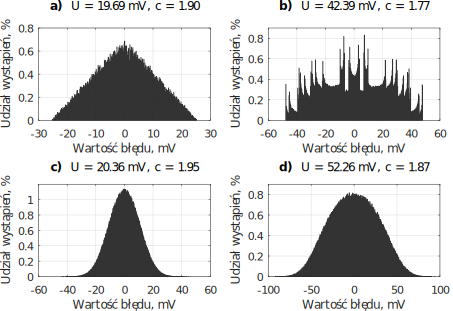
\includegraphics{obrazki/hist_part_b}
\makecaption{fig:symul_partb_hist}{Histogramy błędów \textbf{a)}~statycznego, \textbf{b)}~dynamicznego, \textbf{c)}~losowego, \textbf{d)}~wypadkowego, wielkości wyjściowej analizowanego w eksperymencie symulacyjnym wzmacniacza pomiarowego uzyskane metodą Monte-Carlo}
\end{center}
\end{figure}

Analizując wyniki eksperymentu zauważyć można, że uzyskane wartości dla sygnałów błędów losowego oraz statycznego są zbliżone do tych przedstawionych w tabeli~\ref{tab:sym_partb_params_unc_sum}. Pozwala to zakładać, że podobnie jak w przypadku analizy właściwości przetwornika pomiarowego, przyjęty model błędu oraz stosowane zależności poprawnie określają związki pomiędzy wskazanymi błędami i umożliwiają poprawne oszacowanie ich parametrów. Na dotychczasowym etapie przeprowadzonej analizy nie wyznaczano wypadkowych parametrów sygnału błędu dynamicznego $e_{b,d}(t)$ oraz sygnału błędu wypadkowego $e_{b,\Sigma}(t)$ -- dane te, jak pokazano na obecnym przykładzie, nie są użyteczne podczas analizy kolejnych fragmentów toru pomiarowego, przy czym zostały one wyznaczone w ramach analizy poprzedniej części tego toru w celu weryfikacji zaproponowanej metody obliczeń.

\section{Analiza przetwornika analogowo-cyfrowego}

Kolejnym elementem wchodzącym w skład analizowanego toru pomiarowego jest przetwornik analogowo-cyfrowy. W eksperymencie zakłada się, że element jest realizowany przy użyciu~\qty{8}{\bitOwego} przetwornika wagowego o zakresie napięcia wejściowego z przedziału $<-3;3>\unit{V}$. Wobec powyższych liczba dostępnych wartości wielkości wyjściowej tego przetwornika wynosi $N_{q} = 2^{8} = 256$, natomiast wartość kwantu jest równa $q = \frac{3 - (-3)~\unit{V}}{256} = \qty{23.44}{mV}$. Zakładając, że wielkością wyjściową $x_{c}(n)$ analizowanego przetwornika będzie dyskretna reprezentacja wielkości wejściowej $y_{b}(t)$, zapisać można na podstawie równań od~\eqref{eq:out_cont_ideal_all} do~\eqref{eq:out_cont_err_sum_all} następujące zależności:
\begin{gather}
\dot{x}_{c} \emb{n} = \dot{y}_{b} \emb{nT_{p}} \label{eq:sym_partc_out_ideal}, \\
\tilde{x}_{c} \emb{n} = \tilde{y}_{b} \emb{nT_{p}} + e_{c,q} \left( \tilde{y}_{b} \emb{nT_{p}} \right) = \dot{x}_{c} \emb{n} + e_{c,\Sigma} \emb{n} \label{eq:sym_partc_out_real}, \\
e_{c,\Sigma} \emb{n} = e_{b,\Sigma} \emb{nT_{p}} + e_{c,q} \left( \tilde{y}_{b} \emb{nT_{p}} \right) \label{eq:sym_partc_error_sum},
\end{gather}
gdzie $T_{p} = \frac{1}{f_{p}} = \qty{20.8(3)}{\micro s}$ jest okresem próbkowania. Na podstawie zależności danych równaniami od~\eqref{eq:adc_function} do~\eqref{eq:adc_qerrrange} zapisać można nierówność określającą przedział, w jakim znajdować się mogą wartości realizacji sygnału błędu kwantowania $e_{c,q}(x)$ jako:
\begin{equation}
\qty{-11.72}{mV} \le e_{c,q} \emb{x} \le \qty{11.72}{mV} \label{eq:sym_partc_error_quant}.
\end{equation}

Analizując równanie~\eqref{eq:sym_partc_out_real} zauważyć można, że realizacja błędu kwantowania zależna jest od wartości przetwarzanej wielkości wejściowej analizowanego przetwornika. Jednakże, jak wykazano w pracach~\cite{sienkowski_kwant, sienkowski_adc}, zależność tą można pominąć. Przy założeniu, że uzyskanie na wejściu przetwornika dowolnej wartości z zakresu wartości wielkości wejściowej jest jednakowo prawdopodobne oraz że podczas pomiaru wielkość ta będzie się zmieniać, błąd kwantowania $e_{c,q}(x)$ rozpatrywać można w kategoriach probabilistycznych jako losową realizację wielkości z zakresu opisanego równaniem~\eqref{eq:sym_partc_error_quant} o rozkładzie jednostajnym~\cite{jakubiec_system}. Takie podejście umożliwia zastosowanie zaproponowanego w pracy modelu błędu, podczas gdy analiza zakładająca funkcję przetwarzania omawianego obiektu daną w postaci równania~\eqref{eq:adc_output} byłaby skomplikowana. Wobec powyższych założeń wariancja $\sigma_{c,rw,q}^{2}$ oraz niepewność rozszerzona $U_{c,rw,q}$ związane z błędem kwantowania $e_{c,q}(x)$ mogą być opisane w postaci:
\begin{gather}
\sigma_{c,rw,q}^{2} = \frac{ q^{2}}{12} = \frac{\emb{\num{23.44e-3}}^{2} }{12} = \qty{45.78}{\micro V} \label{eq:sym_partc_var_quant}, \\
U_{c,rw,q} = c_{u} \sigma_{c,rw,q} = \num{1.65} \cdot \num{6.77e-3} = \qty{11.16}{mV} \label{eq:sym_partc_uncert_quant},
\end{gather}
gdzie zgodnie z założeniami opisanymi w~\cite{gray_quantization, widrow_quantization} przyjmuje się model błędu kwantowania zbliżony do modelu addytywnego szumu o stałej widmowej gęstości mocy i jednakowym prawdopodobieństwie uzyskania każdej z możliwych realizacji tego błędu.

Aby zweryfikować poprawność przedstawionych zależności przeprowadzono eksperyment stosując metodę Monte-Carlo. W ramach eksperymentu wyznaczono sto tysięcy razy wartość wielkości wyjściowej analizowanego obiektu, a następnie porównano ją z wartością idealną, uzyskaną dla fragmentu toru pomiarowego w którym nie występowały żadne źródła błędów. Działanie analizowanego przetwornika opisane było równaniem zgodnym z zależnością~\eqref{eq:adc_output}. Na podstawie uzyskanych zgodnie z równaniem~\eqref{eq:sym_partc_error_sum} wartości realizacji sygnału błędu wyznaczono wariancję tego sygnału oraz niepewność rozszerzoną na podstawie równania~\eqref{eq:unc_summation}. Identyczny eksperyment przeprowadzono ponownie z tą różnicą, że jako jedyne źródło błędów uwzględniono w nim obecność procesu kwantowania w celu oszacowania parametrów błędu kwantowania. Rysunek~\ref{fig:symul_partc_hist} przedstawia uzyskane na drodze eksperymentu histogramy.

\begin{figure}[htb!]
\begin{center}
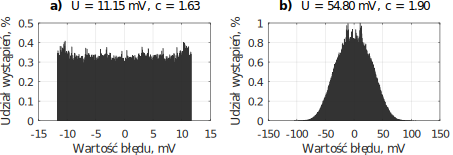
\includegraphics{obrazki/hist_part_c}
\makecaption{fig:symul_partc_hist}{Histogramy błędów \textbf{a)}~kwantowania, \textbf{b)}~wypadkowego, wielkości wyjściowej analizowanego w eksperymencie symulacyjnym przetwornika analogowo-cyfrowego uzyskane metodą Monte-Carlo}
\end{center}
\end{figure}

Analizując wyniki poprzedniego eksperymentu, przedstawione na rysunku~\ref{fig:symul_partb_hist}, oraz wyniki bieżącego eksperymentu, przedstawione na rysunku~\ref{fig:symul_partc_hist}, wnioskować można, że przyjęte założenia są spełnione. Wariancja sygnału błędu wypadkowego $\sigma_{b,\Sigma}^{2}$ wielkości wejściowej przetwornika analogowo-cyfrowego wyniosła~\qty{788.18}{\micro V} w poprzednim eksperymencie. Wariancja sygnału błędu wypadkowego $\sigma_{c,\Sigma}^{2}$ wielkości wyjściowej przetwornika analogowo-cyfrowego wyniosła w bieżącym eksperymencie~\qty{835.18}{\micro V}, wartość wariancji błędu kwantowania $\sigma_{c,rw,q}^{2}$ wyniosła~\qty{46.88}{\micro V}, natomiast związana z nią niepewność rozszerzona $U_{c,rw,q}$ wyniosła~\qty{11.16}{mV}. Uzyskane wartości pokrywają się z wartościami wyznaczonymi na podstawie równań~\eqref{eq:sym_partc_var_quant} oraz~\eqref{eq:sym_partc_uncert_quant}. Korelację pomiędzy sygnałem błędu wypadkowego $e_{b,\Sigma}(t)$ wielkości wejściowej przetwornika analogowo-cyfrowego oraz sygnałem błędu kwantowania $e_{c,rw,q}(n)$ określić można na podstawie równania~\eqref{eq:var_corr}, przy czym:
\begin{equation}
r_{c,rw,q;b,\Sigma} = \frac{\sigma_{c,\Sigma}^{2} - \sigma_{c,rw,q}^{2} - \sigma_{b,\Sigma}^{2}}{2 \sigma_{c,rw,q} \sigma_{b,\Sigma}} = \frac{\num{8.4e-4} - \num{4.7e-5} - \num{7.9e-4}}{2 \cdot \num{6.85e-3} \cdot \num{2.81e-2}} = \num{7.8e-4} \label{eq:sym_partc_corr}.
\end{equation}
Uzyskana wartość współczynnika korelacji oraz wyniki przeprowadzonych eksperymentów świadczą o prawidłowości przyjętych założeń. Wobec powyższych założyć można, że przetwarzane przez analizowany obiekt sygnały błędów przenoszone będą na jego wyjście zgodnie z zależnością:
\begin{gather}
e_{c} \emb{n} \cong e_{b} \emb{nT_{p}} \label{eq:sym_partc_err_prop}, \\
\sigma_{c}^{2} \emb{\omega} \cong \sigma_{b}^{2} \emb{\omega} \label{eq:sym_partc_var_prop},
\end{gather}
a zatem zachowają one swoje oryginalne parametry. Na podstawie przedstawionych zależności oraz tabeli~\ref{tab:sym_partb_params_unc_list} sporządzono budżet niepewności wielkości wyjściowej $x_{c}(n)$ analizowanego przetwornika analogowo-cyfrowego, który zestawiono w tabeli~\ref{tab:sym_partc_params_unc_list}.

\begin{table}[htb!]
\begin{center}
\makecaption{tab:sym_partc_params_unc_list}{Budżet niepewności wielkości wyjściowej analizowanego w eksperymencie symulacyjnym przetwornika analogowo-cyfrowego, gdzie (a) oznacza przetwornik pomiarowy, (b) oznacza wzmacniacz pomiarowy oraz (c) oznacza przetwornik analogowo-cyfrowy}
\begin{tabular}[c]{| c | c | S[table-format = 2.2] | S[table-format = 3.2] | c | c |} \hline
\textbf{Lp.} & \textbf{Symbol} & \textbf{$U$, mV} & \textbf{$\sigma^{2}$, \micro V} & \textbf{Rozkład} & \textbf{Źródło błędu} \\ \hline
1  & ${c,rw,q}$     & 11.16 &  45.78  & jednostajny                  & proces kwantowania (c)                     \\ \hline
2  & ${c,sp,1}$     & 11.52 &  36.75  & trójkątny                    & dryf temperatury (a)                       \\ \hline
3  & ${c,sp,2}$     & 8.15  &  18.38  & trójkątny                    & dryf temperatury (b)                       \\ \hline
4  & ${c,rp,1}$     & 9.93  &  36.26  & jednostajny                  & nieliniowość obiektu (a)                   \\ \hline
5  & ${c,rp,2}$     & 16.70 &  72.64  & normalny                     & szum wielkości wejściowej                  \\ \hline
6  & ${c,dp,a,1}$   & 6.21  &  19.14  & \multirow{6}{*}{dwumodalny}  & \multirow{3}{*}{transmitancja (a)}         \\ \cline{1-4}
7  & ${c,dp,a,2}$   & 15.53 &  119.62 &                              &                                            \\ \cline{1-4}
8  & ${c,dp,a,3}$   & 15.52 &  119.44 &                              &                                            \\ \cline{1-4} \cline{6-6}
9  & ${c,dp,b,1}$   & 3.06  &  4.64   &                              & \multirow{3}{*}{transmitancja (b)}         \\ \cline{1-4}
10 & ${c,dp,b,2}$   & 7.65  &  29.00  &                              &                                            \\ \cline{1-4}
11 & ${c,dp,b,3}$   & 7.65  &  28.99  &                              &                                            \\ \hline
\end{tabular}
\end{center}
\end{table}

Przedstawiony w tabeli~\ref{tab:sym_partc_params_unc_list} budżet niepewności dobrze obrazuje źródła sygnałów błędów występujące w analizowanym torze pomiarowym oraz jednoznacznie wskazuje ich parametry. Na dalszym etapie analizy stosowanie przedstawionego zestawienia jest jednak kłopotliwe, ponieważ wiąże się z koniecznością analizy każdego ze wskazanych sygnałów błędu z osobna. Ze względu na fakt, że proponowany w pracy model błędu dotyczący kolejnego fragmentu toru pomiarowego, jakim jest algorytm transformacji falkowej, wymaga jedynie określenia parametrów wypadkowego sygnału błędu statycznego, losowego oraz wypadkowych parametrów kolejnych harmonicznych sygnału błędu dynamicznego, proponuje się sporządzenie budżetu niepewności uwzględniającego opisywany podział, podobnie jak to miało miejsce w przypadku poprzedniego elementu analizowanego toru pomiarowego.

Parametry opisujące wypadkowy sygnał błędu losowego wyznaczyć można zgodnie z równaniami~\eqref{eq:var_sum} oraz~\eqref{eq:unc_matrix}, które w obecnym przypadku przyjmują postać:
\begin{gather}
\sigma_{c,r}^{2} = \sigma_{c,rp,1}^{2} + \sigma_{c,rp,2}^{2} + \sigma_{c,q}^{2} = \sigma_{b,rp,1}^{2} + \sigma_{b,rp,2}^{2} + \sigma_{c,q}^{2} = \qty{154.68}{\micro V} \label{eq:sym_partc_rand_var}, \\
\begin{split}
U_{c,r} = ~ & \sqrt{
\begin{bmatrix}
U_{c,rp,1} \\ U_{c,rp,2} \\ U_{c,q}
\end{bmatrix}^{T}
\begin{bmatrix}
1            & h_{c,rp,1,2} & h_{c,rp,1,q} \\
h_{c,rp,2,1} & 1            & h_{c,rp,2,q} \\
h_{c,q,rp,1} & h_{c,q,rp,2} & 1
\end{bmatrix}
\begin{bmatrix}
U_{c,rp,1} \\ U_{c,rp,2} \\ U_{c,q}
\end{bmatrix}} = ~ \\ & \sqrt{
\begin{bmatrix}
\num{9.93e-3} \\ \num{16.70e-3} \\ \num{11.16e-3}
\end{bmatrix}^{T}
\begin{bmatrix}
\num{1.000} & \num{0.091} & \num{0.141} \\
\num{0.091} & \num{1.000} & \num{0.103} \\
\num{0.141} & \num{0.103} & \num{1.000}
\end{bmatrix}
\begin{bmatrix}
\num{9.93e-3} \\ \num{16.70e-3} \\ \num{11.16e-3}
\end{bmatrix}} = \qty{24.53}{mV}
\end{split}
\label{eq:sym_partc_rand_uncert}, \\
h_{c,rp,1,2} = s_{u,n} \sqrt{\frac{\num{9.93e-3}}{\num{16.70e-3}}} \left( \frac{\num{98.60e-6} + \num{278.89e-6}}{\num{502.04e-6}} \right) = \num{0.091} \label{eq:sym_partc_coher_rp_1_2}, \\
h_{c,q,rp,1} = s_{u,u} \sqrt{\frac{\num{9.93e-3}}{\num{11.16e-3}}} \left( \frac{\num{98.60e-6} + \num{124.55e-6}}{\num{502.04e-6}} \right) = \num{0.141} \label{eq:sym_partc_coher_q_rp_1}, \\
h_{c,q,rp,2} = s_{u,n} \sqrt{\frac{\num{11.16e-3}}{\num{16.70e-3}}} \left( \frac{\num{124.55e-6} + \num{278.89e-6}}{\num{502.04e-6}} \right) = \num{0.103} \label{eq:sym_partc_coher_q_rp_2}, \\
c_{c,r} = \frac{U_{c,r}}{\sigma_{c,r}} = \frac{\num{24.53e-3}}{\num{12.44e-3}} = \num{1.97} \label{eq:sym_partc_rand_factor}.
\end{gather}

Na podstawie wyznaczonej w równaniu~\eqref{eq:sym_partc_rand_factor} wartości współczynnika rozszerzenia oraz ze względu na spełnienie w analizowanym przypadku warunków centralnego twierdzenia granicznego, zakładać można normalny rozkład wypadkowego sygnału błędu losowego. Biorąc pod uwagę przedstawione dotychczas założenia, wyniki zawarte w tabelach~\ref{tab:sym_partb_params_unc_sum} oraz~\ref{tab:sym_partc_params_unc_list}, jak również wyniki obliczeń przedstawionych w równaniach~\eqref{eq:sym_partc_rand_var} oraz~\eqref{eq:sym_partc_rand_uncert}, sporządzono budżet niepewności z uwzględnieniem omawianego wcześniej podziału, który zestawiono w tabeli~\ref{tab:sym_partc_params_unc_sum}.

\begin{table}[htb!]
\begin{center}
\makecaption{tab:sym_partc_params_unc_sum}{Budżet niepewności wielkości wyjściowej analizowanego w eksperymencie symulacyjnym przetwornika analogowo-cyfrowego z uwzględnieniem podziału na wypadkowe sygnały błędów statycznych, dynamicznych oraz losowych}
\begin{tabular}[c]{| c | c | S[table-format = 2.2] | S[table-format = 3.2] | c | c |} \hline
\textbf{Lp.} & \textbf{Symbol} & \textbf{$U$, mV} & \textbf{$\sigma^{2}$, \micro V} & \textbf{Rozkład} & \textbf{Źródło błędu} \\ \hline
1 & ${c,s}$        & 19.67 &  107.12 & trójkątny                    & wypadkowy dryf temperatury                 \\ \hline
2 & ${c,r}$        & 24.53 &  154.68 & normalny                     & szum, nieliniowość, konwersja              \\ \hline
3 & ${c,d,1}$      & 9.20  &  42.60  & \multirow{3}{*}{dwumodalny}  & \multirow{3}{*}{wypadkowa transmitancja}   \\ \cline{1-4}
4 & ${c,d,2}$      & 23.01 &  266.34 &                              &                                            \\ \cline{1-4}
5 & ${c,d,3}$      & 23.00 &  266.11 &                              &                                            \\ \hline
\end{tabular}
\end{center}
\end{table}

\section{Analiza algorytmu transformacji falkowej}

Ostatnim, przy czym najistotniejszym z punktu widzenia pracy, fragmentem analizowanego toru pomiarowego jest algorytm dyskretnej transformacji falkowej. Zakłada się, że dla każdej $k$-tej realizacji pomiaru na wejście algorytmu podawany jest wektor wielkości wejściowych $\mathbf{x}_{d}(k)$ złożony z $N = 8$ występujących po sobie próbek wielkości wyjściowej $x_{c}(i)$ przetwornika analogowo-cyfrowego. Wyjście analizowanego algorytmu stanowi wektor $\mathbf{X}(k)$ składający się z $M = 8$ wielkości, które stanowią ostateczne wielkości wyjściowe analizowanego toru pomiarowego. Omawiany algorytm wykorzystuje falkę \enquote{db2}, przy czym na jego realizację składają się dwie iteracje procesu dekompozycji sygnału. Macierz transformacji $\mathbf{A}$ omawianego algorytmu przedstawia równanie~\eqref{eq:db2_2_8_matrix}. Zakłada się, że implementacja stosowanego algorytmu wykorzystuje liczby zmiennoprzecinkowe połowicznej precyzji, o długości słowa~\qty{16}{\bitOw}~\cite{gcc_manual}.

Wobec powyższych założeń oraz modelu zaproponowanego w równaniach od~\eqref{eq:alg_out_mat} do~\eqref{eq:alg_out_single} wektor wielkości wejściowych analizowanego algorytmu opisać można w postaci:
\begin{gather}
\dot{\mathbf{x}}_{d}^{T} \emb{k} =
\begin{bmatrix}
\dot{x}_{c} \emb{kT_{p}} & \dot{x}_{c} \left( \emb{k+1} T_{p} \right) & \hdots & \dot{x}_{c} \left( \emb{k+7} T_{p} \right)
\end{bmatrix}
\label{eq:sym_partd_input_ideal}, \\
\tilde{\mathbf{x}}_{d}^{T} \emb{k} =
\begin{bmatrix}
\tilde{x}_{c} \emb{kT_{p}} & \tilde{x}_{c} \left( \emb{k+1} T_{p} \right) & \hdots & \tilde{x}_{c} \left( \emb{k+7} T_{p} \right)
\end{bmatrix}
\label{eq:sym_partd_input_real}.
\end{gather}
Wektor realizacji sygnału błędu wielkości wyjściowych algorytmu opisuje równanie:
\begin{equation}
\mathbf{e}_{d,\Sigma}^{T} \emb{k} =
\begin{bmatrix}
e_{c,\Sigma} \emb{kT_{p}} & e_{c,\Sigma} \left( \emb{k+1} T_{p} \right) & \hdots & e_{c,\Sigma} \left( \emb{k+7} T_{p} \right)
\end{bmatrix}
\label{eq:sym_partd_input_error_sum}.
\end{equation}
Dodatkowo zdefiniować można wektory realizacji sygnałów błędów rozpatrując zaproponowany podział na błędy statyczne, losowe oraz dynamiczne:
\begin{gather}
\mathbf{e}_{d,s}^{T} \emb{k} =
\begin{bmatrix}
e_{c,s} \emb{kT_{p}} & e_{c,s} \left( \emb{k+1} T_{p} \right) & \hdots & e_{c,s} \left( \emb{k+7} T_{p} \right)
\end{bmatrix}
\label{eq:sym_partd_input_error_stat}, \\
\mathbf{e}_{d,r}^{T} \emb{k} =
\begin{bmatrix}
e_{c,r} \emb{kT_{p}} & e_{c,r} \left( \emb{k+1} T_{p} \right) & \hdots & e_{c,r} \left( \emb{k+7} T_{p} \right)
\end{bmatrix}
\label{eq:sym_partd_input_error_rand}, \\
\mathbf{e}_{d,d}^{T} \emb{k} =
\begin{bmatrix}
e_{c,d} \emb{kT_{p}} & e_{c,d} \left( \emb{k+1} T_{p} \right) & \hdots & e_{c,d} \left( \emb{k+7} T_{p} \right)
\end{bmatrix}
\label{eq:sym_partd_input_error_dyn},
\end{gather}
a także w analogiczny sposób rozpatrywać można wektory sygnałów błędów cząstkowych, których parametry zestawiono w tabeli~\ref{tab:sym_partc_params_unc_list}. Wobec powyższego, zgodnie z równaniem~\eqref{eq:alg_out_mul}, wektor wielkości wyjściowych opisać można jako:
\begin{gather}
\dot{\mathbf{X}} \emb{k} = \mathbf{A} \cdot \dot{\mathbf{x}}_{d} \emb{k} \label{eq:sym_partd_output_ideal}, \\
\tilde{\mathbf{X}} \emb{k} = \mathbf{A} \cdot \tilde{\mathbf{x}}_{d} \emb{k} + \mathbf{e}_{d,z} \emb{k} = \dot{\mathbf{X}} \emb{k} + \mathbf{e}_{X,\Sigma} \emb{k} \label{eq:sym_partd_output_real},
\end{gather}
gdzie $\mathbf{e}_{d,z}(k)$ jest wektorem realizacji błędu własnego zaokrągleń $e_{d,z}(j)$, natomiast kolejne wektory realizacji sygnałów błędów wielkości wyjściowej są opisane w postaci:
\begin{gather}
\mathbf{e}_{X,\Sigma} \emb{k} = \mathbf{A} \cdot \mathbf{e}_{d,\Sigma} \emb{k} = \mathbf{e}_{X,s} \emb{k} + \mathbf{e}_{X,d} \emb{k} + \mathbf{e}_{X,r} \emb{k} + \mathbf{e}_{d,z} \emb{k} \label{eq:sym_partd_output_error_sum}, \\
\mathbf{e}_{X,s} \emb{k} = \mathbf{A} \cdot \mathbf{e}_{d,s} \emb{k} \label{eq:sym_partd_output_error_stat}, \\
\mathbf{e}_{X,d} \emb{k} = \mathbf{A} \cdot \mathbf{e}_{d,d} \emb{k} \label{eq:sym_partd_output_error_dyn}, \\
\mathbf{e}_{X,r} \emb{k} = \mathbf{A} \cdot \mathbf{e}_{d,r} \emb{k} \label{eq:sym_partd_output_error_rand}.
\end{gather}

Należy zauważyć, że tak jak w przypadku wektora wielkości wejściowych, tak i w przypadku wektora wielkości wyjściowych, wyróżnić można również osobne wektory realizacji sygnałów błędów dla każdego z opisanych w tabeli~\ref{tab:sym_partc_params_unc_list} sygnałów. Zgodnie z oznaczeniami przyjętymi w równaniach~\eqref{eq:db2_invect} oraz~\eqref{eq:db2_outvect}, wektory wielkości wejściowych $\mathbf{x}(k)$ i wyjściowych $\mathbf{X}(k)$ pojedynczej realizacji algorytmu dla $k$-tego okna pomiarowego są w dalszej części rozdziału oznaczane symbolami:
\begin{gather}
\mathbf{x}_{d}^{T} =
\begin{bmatrix}
S_{0,0} & S_{0,1} & S_{0,2} & S_{0,3} & S_{0,4} & S_{0,5} & S_{0,6} & S_{0,7}
\end{bmatrix}
\label{eq:sym_partd_invect}, \\
\mathbf{X}^{T} =
\begin{bmatrix}
S_{2,0} & S_{2,1} & T_{2,0} & T_{2,1} & T_{1,0} & T_{1,1} & T_{1,2} & T_{1,3}
\end{bmatrix}
\label{eq:sym_partd_outvect},
\end{gather}
natomiast wektor realizacji sygnałów błędów wielkości wyjściowej  $\mathbf{e}_{X,*}(k)$ dla pojedynczej $k$-tej iteracji realizacji algorytmu jest oznaczany w postaci:
\begin{equation}
\mathbf{e}_{X,*}^{T} =
\begin{bmatrix}
e_{S_{2,0},*} & e_{S_{2,1},*} & e_{T_{2,0},*} & e_{T_{2,1},*} & e_{T_{1,0},*} & e_{T_{1,1},*} & e_{T_{1,2},*} & e_{T_{1,3},*}
\end{bmatrix}
\label{eq:sym_partd_errvect},
\end{equation}
gdzie w miejsce symbolu \enquote{$*$} umieszczany jest symbol analizowanego sygnału błędu.

W poprzednich podrozdziałach przedstawiono różne sposoby wyznaczania budżetu niepewności, uwzględniające każde źródło błędu z osobna oraz wskazujące wypadkowe parametry danego rodzaju błędu. Zabiegi te miały na celu wskazanie optymalnej drogi analizy właściwości metrologicznych z punktu widzenia projektanta toru pomiarowego, tak aby nie wykonywał on czynności nieistotnych z punktu widzenia przeprowadzanej analizy. Opisywany zabieg został również przeprowadzony w celu weryfikacji postawionej w pracy tezy, jako przy wykorzystaniu zaproponowanej metody analizy istnieje możliwość wyznaczenia jedynie zastępczych parametrów sygnałów błędów wielkości wejściowej algorytmu dyskretnej transformacji falkowej w celu oszacowania wartości niepewności na wyjściu tego algorytmu. W dalszej części rozdziału opisane zostały dwa sposoby wyznaczenia niepewności wielkości wyjściowych algorytmu. Podejście pierwsze uwzględniać będzie budżet niepewności podzielony na kategorie błędów, opisany w tabeli~\ref{tab:sym_partc_params_unc_sum}, natomiast podejście drugie przedstawi analizę z wykorzystaniem budżetu sporządzonego dla każdego sygnału błędu z osobna, który przedstawiono w tabeli~\ref{tab:sym_partc_params_unc_list}.

Istotnym faktem podczas analizy właściwości metrologicznych stosowanego algorytmu jest to, że jego wielkości wejściowe każdorazowo pochodzą z tego samego źródła. Powtarzając proces wyznaczania wartości wektora wielkości wyjściowych algorytmu wielokrotnie, wszystkie wielkości wejściowe algorytmu cechowały będą te same parametry wariancji i niepewności rozszerzonej. Zjawisko to zostało omówione w poprzedniej części pracy. Ze względu na fakt, że w przypadku błędów o charakterze statycznym, wartości realizacji tych błędów nie zmieniają się w obrębie pojedynczego okna pomiarowego, do oceny wariancji wyjściowego sygnału związanego z tym rodzajem błędu stosowane będzie równanie~\eqref{eq:alg_outvar_stat}. Do określenia parametrów sygnałów błędów o charakterze dynamicznym wykorzystana zostanie transmitancja pojedynczej wielkości wyjściowej algorytmu dana równaniem~\eqref{eq:alg_trans_single}, natomiast w przypadku sygnałów błędów o charakterze losowym wykorzystywana będzie w tym celu zależność~\eqref{eq:alg_outvar_rand}, ze względu na stałą widmową gęstość mocy tych sygnałów w zakresie częstotliwości $\hat{f} \in~<0;\frac{1}{2} f_{p}>$.
Przedstawiane w dalszej części obliczenia dotyczą dwóch przykładowych wielkości wyjściowych algorytmu -- $S_{2,0}$ oraz $T_{1,0}$. Wybór przedstawionych wielkości jest uzasadniony faktem, że jedna z nich stanowi detale sygnału (jest reprezentowana przez filtr dolno-przepustowy związany z funkcją skalującą), natomiast druga stanowi aproksymacje sygnału (jest reprezentowana przez filtr pasmowo-przepustowy związany z falką-matką). Pozostałe wielkości poddano analizie w identyczny sposób, natomiast dla zachowania czytelności pracy obliczenia te nie zostały przedstawione.

Błędy statyczne przenoszone są przez analizowany algorytm z wejścia na wyjście zgodnie z równaniem~\eqref{eq:alg_outerr_stat}, a zatem zgodnie z zależnością~\eqref{eq:alg_outvar_stat} może zostać wyznaczona ich wariancja, przy czym na etapie analizy dla każdej wielkości wyjściowej wyznaczana jest wartość współczynnika $A_{s}$, zgodnie z równaniem~\eqref{eq:alg_trans_stat}. W przypadku błędów losowych, przenoszonych zgodnie z zależnością~\eqref{eq:alg_outerr} ich wariancja jest wyznaczana zgodnie z równaniem~\eqref{eq:alg_outvar_rand} i, podobnie jak w przypadku błędów statycznych, do jej wyznaczenia stosowane są współczynniki $A_{r}$ wyznaczone zgodnie z zależnością~\eqref{eq:alg_trans_rand}. Można zatem dla rozważanych wielkości wyjściowych zapisać:
\begin{gather}
A_{S_{2,0},s} = \sum _{j = 0} ^{N-1} a_{0, j} = 2 \label{eq:sym_partd_output_as_S_2_0}, \\
A_{S_{2,0},r} = \sqrt{\sum _{j = 0} ^{N-1} a_{0, j}^{2}} = 1 \label{eq:sym_partd_output_ar_S_2_0}, \\
A_{T_{1,0},s} = \sum _{j = 0} ^{N-1} a_{4, j} = 0 \label{eq:sym_partd_output_as_T_1_0}, \\
A_{T_{1,0},r} = \sqrt{\sum _{j = 0} ^{N-1} a_{4, j}^{2}} = 1 \label{eq:sym_partd_output_ar_T_1_0}.
\end{gather}
Należy zauważyć, że zgodnie z oczekiwaniami wielkość wyjściowa $T_{1,0}$ nie będzie obarczona błędem statycznym w związku z faktem, że jest ona związana z filtrem pasmowo-przepustowym. Dodatkowo zauważyć można, że dla wszystkich wielkości wyjściowych współczynnik $A_{r}$ każdorazowo będzie równy jedności, co wynika z założenia rodziny \enquote{Daubechies} odnośnie normalizacji energii~\cite{vonesch_dbbasics, wei_coiflet}.

Zgodnie z równaniem~\eqref{eq:alg_trans_single} oraz postacią macierzy $\mathbf{A}$ daną równaniem~\eqref{eq:db2_2_8_matrix}, transmitancje algorytmu związane z omawianymi wielkościami wyjściowymi w dziedzinie $\mathcal{Z}$ przedstawiają następujące równania:
\begin{gather}
\begin{split}
H_{S_{2,0}} \emb{z} = ~
& \frac{5 - \sqrt{3}}{16} + \frac{5 + \sqrt{3}}{16} z^{-1} + \frac{3 + 3 \sqrt{3}}{16} z^{-2} + \frac{5 + 3 \sqrt{3}}{16} z^{-3} + \\
& \frac{3 + \sqrt{3}}{16} z^{-4} + \frac{3 - \sqrt{3}}{16} z^{-5} + \frac{5 - 3 \sqrt{3}}{16} z^{-6} + \frac{3 - 3 \sqrt{3}}{16} z^{-7}
\end{split}
\label{eq:sym_partd_output_trans_z_S_2_0}, \\
H_{T_{1,0}} \emb{z} = \frac{1 - \sqrt{3}}{4 \sqrt{2}} - \frac{3 - \sqrt{3}}{4 \sqrt{2}} z^{-1} + \frac{3 + \sqrt{3}}{4 \sqrt{2}} z^{-2} - \frac{1 + \sqrt{3}}{4 \sqrt{2}} z^{-3} \label{eq:sym_partd_output_trans_z_T_1_0}.
\end{gather}
Podstawiając do powyższych równań założenie gdzie $z = e^{j\omega_{n}}$ otrzymuje się zależności opisujące transmitancje wybranych wierszy w funkcji pulsacji znormalizowanej~\cite{oppenheim_dsp}:
\begin{gather}
\begin{split}
G_{S_{2,0}} \emb{\omega_{n}} = ~
& \frac{5 - \sqrt{3}}{16} + \frac{5 + \sqrt{3}}{16} e^{-j\omega_{n}} + \frac{3 + 3 \sqrt{3}}{16} e^{-2j\omega_{n}} + \\
& \frac{5 + 3 \sqrt{3}}{16} e^{-3j\omega_{n}} + \frac{3 + \sqrt{3}}{16} e^{-4j\omega_{n}} + \frac{3 - \sqrt{3}}{16} e^{-5j\omega_{n}} + \\
& \frac{5 - 3 \sqrt{3}}{16} e^{-6j\omega_{n}} + \frac{3 - 3 \sqrt{3}}{16} e^{-7j\omega_{n}}
\end{split}
\label{eq:sym_partd_output_trans_wn_S_2_0}, \\
G_{T_{1,0}} \emb{\omega_{n}} = \frac{1 - \sqrt{3}}{4 \sqrt{2}} - \frac{3 - \sqrt{3}}{4 \sqrt{2}} e^{-j\omega_{n}} + \frac{3 + \sqrt{3}}{4 \sqrt{2}} e^{-2j\omega_{n}} - \frac{1 + \sqrt{3}}{4 \sqrt{2}} e^{-3j\omega_{n}} \label{eq:sym_partd_output_trans_wn_T_1_0},
\end{gather}
przy czym pulsacja znormalizowana $\omega_{n} = \omega T_{p}$ dla okresu próbkowania $T_{p}$. Wobec powyższych, zgodnie z zależnościami~\eqref{eq:mid_disc_amp} oraz~\eqref{eq:mid_disc_phi}, wyznaczyć można wzmocnienie oraz przesunięcie fazowe dla analizowanych wielkości wyjściowych w funkcji pulsacji oraz wskazać można rzeczywistą i urojoną część transmitancji analizowanych wielkości:
\begin{gather}
\begin{split}
\Re \left( G_{S_{2,0}} \emb{\omega} \right) = ~
& \frac{5 + \sqrt{3}}{16} \cos \emb{\omega T_{p}} + \frac{3 + 3 \sqrt{3}}{16} \cos \emb{2 \omega T_{p}} + \\
& \frac{5 + 3 \sqrt{3}}{16} \cos \emb{3 \omega T_{p}} + \frac{3 + \sqrt{3}}{16} \cos \emb{4 \omega T_{p}} + \\
& \frac{3 - \sqrt{3}}{16} \cos \emb{5 \omega T_{p}} + \frac{5 - 3 \sqrt{3}}{16} \cos \emb{6 \omega T_{p}} + \\
& \frac{3 - 3 \sqrt{3}}{16} \cos \emb{7 \omega T_{p}} + \frac{5 - \sqrt{3}}{16}
\end{split}
\label{eq:sym_partd_output_trans_wn_re_S_2_0}, \\
\begin{split}
\Im \left( G_{S_{2,0}} \emb{\omega} \right) = ~
& - \frac{5 + \sqrt{3}}{16} \sin \emb{\omega T_{p}} - \frac{3 + 3 \sqrt{3}}{16} \sin \emb{2 \omega T_{p}} \\
& - \frac{5 + 3 \sqrt{3}}{16} \sin \emb{3 \omega T_{p}} - \frac{3 + \sqrt{3}}{16} \sin \emb{4 \omega T_{p}} \\
& - \frac{3 - \sqrt{3}}{16} \sin \emb{5 \omega T_{p}} - \frac{5 - 3 \sqrt{3}}{16} \sin \emb{6 \omega T_{p}} \\
& - \frac{3 - 3 \sqrt{3}}{16} \sin \emb{7 \omega T_{p}}
\end{split}
\label{eq:sym_partd_output_trans_wn_im_S_2_0}, \\
\begin{split}
\Re \left( G_{T_{1,0}} \emb{\omega} \right) = ~
& - \frac{3 - \sqrt{3}}{4 \sqrt{2}} \cos \emb{\omega T_{p}} + \frac{3 + \sqrt{3}}{4 \sqrt{2}} \cos \emb{2 \omega T_{p}} \\
& - \frac{1 + \sqrt{3}}{4 \sqrt{2}} \cos \emb{3 \omega T_{p}} + \frac{1 - \sqrt{3}}{4 \sqrt{2}}
\end{split}
\label{eq:sym_partd_output_trans_wn_re_T_1_0}, \\
\begin{split}
\Im \left( G_{T_{1,0}} \emb{\omega} \right) = ~
& \frac{3 - \sqrt{3}}{4 \sqrt{2}} \sin \emb{\omega T_{p}} - \frac{3 + \sqrt{3}}{4 \sqrt{2}} \sin \emb{2 \omega T_{p}} + \\
& \frac{1 + \sqrt{3}}{4 \sqrt{2}} \sin \emb{3 \omega T_{p}}
\end{split}
\label{eq:sym_partd_output_trans_wn_im_T_1_0}.
\end{gather}

Przedstawione zależności pozwalają zgodnie z równaniem~\eqref{eq:mid_disc_err_dyn_prop} określić w jaki sposób algorytm przenosi z wejścia na wyjście obecne w przetwarzanym sygnale harmoniczne sygnału błędu dynamicznego. Zgodnie z wcześniejszymi założeniami przyjmuje się, że przedstawiana transmitancja algorytmu jest transmitancją idealną, a zatem obiekt ten nie wprowadza błędu dynamicznego własnego do wielkości wyjściowych. Jako, że analizowany algorytm jest ostatnim elementem rozważanego toru pomiarowego, z punktu widzenia właściwości metrologicznych istotna jest jedynie amplituda kolejnych harmonicznych sygnału błędu dynamicznego, która pozwoli oszacować wariancję związaną z analizowaną częstotliwością sygnału błędu. Znajomość fazy przetwarzanej harmonicznej błędu dynamicznego będzie istotna tylko wtedy, gdy zaistnieje konieczność wyznaczania wypadkowych parametrów kilku harmonicznych o tej samej pulsacji. Parametry wypadkowe harmonicznych sygnału błędu dynamicznego są wyznaczane zgodnie z zależnościami od~\eqref{eq:dyn_vect} do~\eqref{eq:dyn_vect_phi}, natomiast do wyznaczenia ich wariancji stosowane jest równanie~\eqref{eq:dyn_var}.

Na podstawie danych zawartych w tabeli~\ref{tab:sym_partc_params_unc_sum} oraz równania~\eqref{eq:sym_partd_output_as_S_2_0} parametry wariancji sygnałów błędów propagowanych statycznych dla wielkości wyjściowej $S_{2,0}$ wyznaczyć można zgodnie z zależnością~\eqref{eq:alg_outvar_trans_stat}:
\begin{equation}
\sigma_{S_{2,0},s}^{2} = \sigma_{c,s}^{2} A_{S_{2,0},s}^{2} = 2^{2} \cdot \num{107.12e-6} = \qty{428.48}{\micro V} \label{eq:sym_partd_output_var_stat_S_2_0},
\end{equation}
natomiast na podstawie równania~\eqref{eq:sym_partd_output_ar_S_2_0} wariancja propagowanego sygnału błędu losowego może być wyznaczona zgodnie z zależnością~\eqref{eq:alg_outvar_trans_rand}:
\begin{equation}
\sigma_{S_{2,0},r}^{2} = \sigma_{c,r}^{2} A_{S_{2,0},r}^{2} = 1^{2} \cdot \num{154.68e-6} = \qty{154.68}{\micro V} \label{eq:sym_partd_output_var_rand_S_2_0}.
\end{equation}
W przypadku sygnałów błędów dynamicznych wariancje kolejnych harmonicznych tych sygnałów wyznaczyć można na podstawie zależności~\eqref{eq:dyn_var} oraz~\eqref{eq:alg_outvar_dyn}:
\begin{gather}
\sigma_{S_{2,0},d,1}^{2} = \sigma_{c,d,1}^{2} K_{S_{2,0}}^{2} \emb{\omega_{c,e,1}} = \num{1.998}^{2} \cdot \num{42.60e-6} = \qty{170.04}{\micro V} \label{eq:sym_partd_output_var_dyn_1_S_2_0}, \\
\sigma_{S_{2,0},d,2}^{2} = \sigma_{c,d,2}^{2} K_{S_{2,0}}^{2} \emb{\omega_{c,e,2}} = \num{1.623}^{2} \cdot \num{266.34e-6} = \qty{704.44}{\micro V} \label{eq:sym_partd_output_var_dyn_2_S_2_0}, \\
\sigma_{S_{2,0},d,3}^{2} = \sigma_{c,d,3}^{2} K_{S_{2,0}}^{2} \emb{\omega_{c,e,3}} = \num{0.152}^{2} \cdot \num{266.11e-6} = \qty{6.18}{\micro V} \label{eq:sym_partd_output_var_dyn_3_S_2_0}.
\end{gather}
Ze względu na brak korelacji przedstawionych sygnałów błędów wariancję sygnału błędu wypadkowego wyznaczyć można zgodnie z równaniem~\eqref{eq:var_sum}, jako sumę wariancji kolejnych sygnałów błędów cząstkowych, wobec czego zachodzi zależność:
\begin{equation}
\sigma_{S_{2,0},\Sigma}^{2} = \sigma_{S_{2,0},z}^{2} + \sigma_{S_{2,0},s}^{2} + \sigma_{S_{2,0},r}^{2} + \sigma_{S_{2,0},d,1}^{2} + \sigma_{S_{2,0},d,2}^{2} + \sigma_{S_{2,0},d,3}^{2} = \qty{1464.79}{\micro V} \label{eq:sym_partd_output_var_sum_S_2_0},
\end{equation}
gdzie $\sigma_{S_{2,0},z}^{2}$ jest wariancją błędu własnego zaokrągleń i zgodnie z tabelą~\ref{tab:varnum_db2_2_f16} wynosi w rozpatrywanym przypadku~\qty{0.974}{\micro V}, natomiast współczynnik rozszerzenia $c_{z}$ jest równy~\num{2.16}.
Zgodnie z zależnościami zachodzącymi w równaniach od~\eqref{eq:sym_partd_output_var_stat_S_2_0} do~\eqref{eq:sym_partd_output_var_dyn_3_S_2_0}, kolejne wartości niepewności rozszerzonych sygnałów błędów cząstkowych wielkości wyjściowej $S_{2,0}$ wynoszą odpowiednio:
\begin{gather}
U_{S_{2,0},z} = c_{z} \sigma_{S_{2,0},z} = \num{2.16} \cdot \num{0.987e-3} = \qty{2.13}{mV} \label{eq:sym_partd_output_unc_roun_S_2_0},\\
U_{S_{2,0},s} = c_{t} \sigma_{S_{2,0},s} = \num{1.90} \cdot \num{20.70e-3} = \qty{39.33}{mV} \label{eq:sym_partd_output_unc_stat_S_2_0}, \\
U_{S_{2,0},r} = c_{n} \sigma_{S_{2,0},r} = \num{1.96} \cdot \num{12.44e-3} = \qty{24.38}{mV} \label{eq:sym_partd_output_unc_rand_S_2_0}, \\
U_{S_{2,0},d,1} = c_{d} \sigma_{S_{2,0},d,1} = \num{1.41} \cdot \num{13.04e-3} = \qty{18.39}{mV} \label{eq:sym_partd_output_unc_dyn_1_S_2_0}, \\
U_{S_{2,0},d,2} = c_{d} \sigma_{S_{2,0},d,2} = \num{1.41} \cdot \num{26.54e-3} = \qty{37.42}{mV} \label{eq:sym_partd_output_unc_dyn_2_S_2_0}, \\
U_{S_{2,0},d,3} = c_{d} \sigma_{S_{2,0},d,3} = \num{1.41} \cdot \num{2.49e-3} = \qty{3.50}{mV} \label{eq:sym_partd_output_unc_dyn_3_S_2_0}.
\end{gather}
Przedstawione zależności stanowią dane niezbędne do wyznaczenie wypadkowej wartości niepewności rozszerzonej związanej z analizowaną wielkością wyjściową algorytmu.

Wyznaczenie wypadkowej wartości niepewności rozszerzonej odbywa się zgodnie z zależnością~\eqref{eq:unc_matrix}. Wymagane jest zatem wyznaczenie wzajemnych relacji pomiędzy składanymi niepewnościami cząstkowymi w postaci macierzy koherencji, której wartości są wyznaczane zgodnie z równaniem~\eqref{eq:unc_coher}. Można zatem zapisać, że:
\begin{equation}
U_{S_{2,0},\Sigma} = \sqrt{\mathbf{U}_{S_{2,0}} \cdot \mathbf{h}_{S_{2,0}} \cdot \mathbf{U}_{S_{2,0}}^{T}} \label{eq:sym_partd_output_unc_summul_S_2_0},
\end{equation}
gdzie symbolem $\mathbf{U}_{S_{2,0}}$ oznaczono wektor cząstkowych niepewności rozszerzonych:
\begin{equation}
\mathbf{U}_{S_{2,0}} =
\begin{bmatrix}
U_{S_{2,0},z} & U_{S_{2,0},s} & U_{S_{2,0},r} & U_{S_{2,0},d,1} & U_{S_{2,0},d,2} & U_{S_{2,0},d,3}
\end{bmatrix}
\label{eq:sym_partd_output_unc_sumuvect_S_2_0_a},
\end{equation}
natomiast macierz koherencji oznaczona symbolem $\mathbf{h}_{S_{2,0}}$ jest dana w postaci:
\begin{equation}
\mathbf{h}_{S_{2,0}} =
\begin{bmatrix}
1                 & h_{S_{2,0},z,s}   & h_{S_{2,0},z,r}   & h_{S_{2,0},z,d,1} & h_{S_{2,0},z,d,2} & h_{S_{2,0},z,d,3} \\
h_{S_{2,0},s,z}   & 1                 & h_{S_{2,0},s,r}   & h_{S_{2,0},s,d,1} & h_{S_{2,0},s,d,2} & h_{S_{2,0},s,d,3} \\
h_{S_{2,0},r,z}   & h_{S_{2,0},r,s}   & 1                 & h_{S_{2,0},r,d,1} & h_{S_{2,0},r,d,2} & h_{S_{2,0},r,d,3} \\
h_{S_{2,0},d,1,z} & h_{S_{2,0},d,1,s} & h_{S_{2,0},d,1,r} & 1                 & h_{S_{2,0},d,1,2} & h_{S_{2,0},d,1,3} \\
h_{S_{2,0},d,2,z} & h_{S_{2,0},d,2,s} & h_{S_{2,0},d,2,r} & h_{S_{2,0},d,2,1} & 1                 & h_{S_{2,0},d,2,3} \\
h_{S_{2,0},d,3,z} & h_{S_{2,0},d,3,s} & h_{S_{2,0},d,3,r} & h_{S_{2,0},d,3,1} & h_{S_{2,0},d,3,2} & 1                 \\
\end{bmatrix}
\label{eq:sym_partd_output_unc_sumcoher_S_2_0}.
\end{equation}
Podstawiając do powyższych zależności wyprowadzone w równaniach od~\eqref{eq:sym_partd_output_unc_roun_S_2_0} do~\eqref{eq:sym_partd_output_unc_dyn_3_S_2_0} wielkości oraz wyznaczając zgodnie z równaniem~\eqref{eq:unc_coher} kolejne wartości współczynników koherencji dla analizowanych danych oraz wartości współczynników kształtu zestawionych w tabelach~\ref{tab:unc_shapefac} oraz~\ref{tab:unc_shapedwt} otrzymuje się:
\begin{gather}
\mathbf{h}_{S_{2,0}} =
\begin{bmatrix}
\num{1.000} & \num{0.000} & \num{0.000} & \num{0.006} & \num{0.017} & \num{0.001} \\
\num{0.000} & \num{1.000} & \num{0.011} & \num{0.116} & \num{0.259} & \num{0.042} \\
\num{0.000} & \num{0.011} & \num{1.000} & \num{0.062} & \num{0.123} & \num{0.018} \\
\num{0.006} & \num{0.116} & \num{0.062} & \num{1.000} & \num{0.223} & \num{0.028} \\
\num{0.017} & \num{0.259} & \num{0.123} & \num{0.223} & \num{1.000} & \num{0.079} \\
\num{0.001} & \num{0.042} & \num{0.018} & \num{0.028} & \num{0.079} & \num{1.000} \\
\end{bmatrix}
\label{eq:sym_partd_output_unc_sumcoherval_S_2_0_a}, \\
\mathbf{U}_{S_{2,0}} =
\begin{bmatrix}
\num{2.13} & \num{39.31} & \num{24.38} & \num{18.39} & \num{37.42} & \num{3.50}
\end{bmatrix} \cdot \num{e-3}
\label{eq:sym_partd_output_unc_sumuvectval_S_2_0_a}, \\
U_{S_{2,0},\Sigma} = \sqrt{\mathbf{U}_{S_{2,0}} \cdot \mathbf{h}_{S_{2,0}} \cdot \mathbf{U}_{S_{2,0}}^{T}} = \qty{74.00}{mV} \label{eq:sym_partd_output_unc_total_a_S_2_0}.
\end{gather}
Jako, że w analizowanej sytuacji spełnione zostały warunki centralnego twierdzenia granicznego, wyznaczenie wypadkowej wartości niepewności rozszerzonej jest możliwe przyjmując założenie zbliżonego do normalnego kształtu rozkładu wypadkowego sygnału błędu. Wobec przedstawionego założenia wartość wypadkowej niepewności rozszerzonej może zostać oszacowana zgodnie z równaniem~\eqref{eq:unc_sum} dla $c_{S_{2,0},\Sigma} = c_{n}$, zatem:
\begin{equation}
U_{S_{2,0},\Sigma} = c_{n} \cdot \sigma_{S_{2,0},\Sigma} = \num{1.96} \cdot \num{38.27e-3} = \qty{75.01}{mV} \label{eq:sym_partd_output_unc_total_b_S_2_0}.
\end{equation}
Porównując wartości otrzymane stosując zależność~\eqref{eq:sym_partd_output_unc_total_b_S_2_0} z wynikami uzyskanymi w równaniu~\eqref{eq:sym_partd_output_unc_total_a_S_2_0} zauważyć można, że obydwie metody zapewniają podobne wyniki, przy czym metoda pierwsza jest znacznie bardziej skomplikowana i wymaga oszacowania wzajemnych relacji pomiędzy składanymi niepewnościami cząstkowymi. W dalszej cześć podrozdziału wyznaczone wartości zostały porównane z wynikami eksperymentu przeprowadzonego metodą Monte-Carlo w celu weryfikacji ich poprawności.

Analogicznie, jak w przypadku przedstawionych powyżej rozważań, parametry wariancji sygnałów błędów propagowanych dla wielkości wyjściowej $T_{1,0}$ wyznaczyć można w przypadku przetwarzanych przez algorytm błędów statycznych i losowych jako:
\begin{gather}
\sigma_{T_{1,0},s}^{2} = \sigma_{c,s}^{2} A_{T_{1,0},s}^{2} = 0^{2} \cdot \num{107.12e-6} = \qty{0.00}{\micro V} \label{eq:sym_partd_output_var_stat_T_1_0}, \\
\sigma_{T_{1,0},r}^{2} = \sigma_{c,r}^{2} A_{T_{1,0},r}^{2} = 1^{2} \cdot \num{154.68e-6} = \qty{154.68}{\micro V} \label{eq:sym_partd_output_var_rand_T_1_0},
\end{gather}
natomiast w przypadku kolejnych harmonicznych sygnału błędu dynamicznego w postaci:
\begin{gather}
\sigma_{T_{1,0},d,1}^{2} = \sigma_{c,d,1}^{2} K_{T_{1,0}}^{2} \emb{\omega_{c,e,1}} = \num{0.010}^{2} \cdot \num{42.6e-6} = \qty{0.0043}{\micro V} \label{eq:sym_partd_output_var_dyn_1_T_1_0}, \\
\sigma_{T_{1,0},d,2}^{2} = \sigma_{c,d,2}^{2} K_{T_{1,0}}^{2} \emb{\omega_{c,e,2}} = \num{0.244}^{2} \cdot \num{266.34e-6} = \qty{15.89}{\micro V} \label{eq:sym_partd_output_var_dyn_2_T_1_0}, \\
\sigma_{T_{1,0},d,3}^{2} = \sigma_{c,d,3}^{2} K_{T_{1,0}}^{2} \emb{\omega_{c,e,3}} = \num{1.243}^{2} \cdot \num{266.11e-6} = \qty{411.41}{\micro V} \label{eq:sym_partd_output_var_dyn_3_T_1_0}.
\end{gather}
Zgodnie z tabelą~\ref{tab:varnum_db2_2_f16} wariancja błędu własnego zaokrągleń $\sigma_{T_{1,0},z}^{2}$ wynosi w tym przypadku~\qty{0.699}{\micro V}. Wobec powyższych, zgodnie z równaniem~\eqref{eq:var_sum}, wariancję błędu wypadkowego wielkości wyjściowej $T_{1,0}$ opisuje zależność:
\begin{equation}
\sigma_{T_{1,0},\Sigma}^{2} = \sigma_{T_{1,0},z}^{2} + \sigma_{T_{1,0},s}^{2} + \sigma_{T_{1,0},r}^{2} + \sigma_{T_{1,0},d,1}^{2} + \sigma_{T_{1,0},d,2}^{2} + \sigma_{T_{1,0},d,3}^{2} = \qty{582.68}{\micro V} \label{eq:sym_partd_output_var_sum_T_1_0},
\end{equation}
natomiast niepewności rozszerzone analizowanych sygnałów błędów składowych wynoszą:
\begin{gather}
U_{T_{1,0},z} = c_{z} \sigma_{T_{1,0},z} = \num{2.16} \cdot \num{0.836e-3} = \qty{1.81}{mV} \label{eq:sym_partd_output_unc_roun_T_1_0},\\
U_{T_{1,0},s} = c_{t} \sigma_{T_{1,0},s} = \num{1.90} \cdot \num{0} = \qty{0}{mV} \label{eq:sym_partd_output_unc_stat_T_1_0}, \\
U_{T_{1,0},r} = c_{n} \sigma_{T_{1,0},r} = \num{1.96} \cdot \num{12.44e-3} = \qty{24.38}{mV} \label{eq:sym_partd_output_unc_rand_T_1_0}, \\
U_{T_{1,0},d,1} = c_{d} \sigma_{T_{1,0},d,1} = \num{1.41} \cdot \num{0.065e-3} = \qty{0.092}{mV} \label{eq:sym_partd_output_unc_dyn_1_T_1_0}, \\
U_{T_{1,0},d,2} = c_{d} \sigma_{T_{1,0},d,2} = \num{1.41} \cdot \num{3.99e-3} = \qty{5.62}{mV} \label{eq:sym_partd_output_unc_dyn_2_T_1_0}, \\
U_{T_{1,0},d,3} = c_{d} \sigma_{T_{1,0},d,3} = \num{1.41} \cdot \num{20.28e-3} = \qty{28.60}{mV} \label{eq:sym_partd_output_unc_dyn_3_T_1_0}.
\end{gather}
Oznaczając symbolem $\mathbf{U}_{T_{1,0}}$ wektor niepewności cząstkowych oraz symbolem  $\mathbf{h}_{S_{2,0}}$ macierz koherencji związane z analizowaną wielkością $T_{1,0}$, wartość wypadkowej niepewności rozszerzonej tej wielkości wyznaczyć można zgodnie z równaniem~\eqref{eq:unc_matrix}:
\begin{gather}
U_{T_{1,0},\Sigma} = \sqrt{\mathbf{U}_{T_{1,0}} \cdot \mathbf{h}_{T_{1,0}} \cdot \mathbf{U}_{T_{1,0}}^{T}} \label{eq:sym_partd_output_unc_summul_T_1_0}, \\
\mathbf{U}_{T_{1,0}} =
\begin{bmatrix}
U_{T_{1,0},z} & U_{T_{1,0},s} & U_{T_{1,0},r} & U_{T_{1,0},d,1} & U_{T_{1,0},d,2} & U_{T_{1,0},d,3}
\end{bmatrix}
\label{eq:sym_partd_output_unc_sumuvect_T_1_0_a}, \\
\mathbf{h}_{T_{1,0}} =
\begin{bmatrix}
1                 & h_{T_{1,0},z,s}   & h_{T_{1,0},z,r}   & h_{T_{1,0},z,d,1} & h_{T_{1,0},z,d,2} & h_{T_{1,0},z,d,3} \\
h_{T_{1,0},s,z}   & 1                 & h_{T_{1,0},s,r}   & h_{T_{1,0},s,d,1} & h_{T_{1,0},s,d,2} & h_{T_{1,0},s,d,3} \\
h_{T_{1,0},r,z}   & h_{T_{1,0},r,s}   & 1                 & h_{T_{1,0},r,d,1} & h_{T_{1,0},r,d,2} & h_{T_{1,0},r,d,3} \\
h_{T_{1,0},d,1,z} & h_{T_{1,0},d,1,s} & h_{T_{1,0},d,1,r} & 1                 & h_{T_{1,0},d,1,2} & h_{T_{1,0},d,1,3} \\
h_{T_{1,0},d,2,z} & h_{T_{1,0},d,2,s} & h_{T_{1,0},d,2,r} & h_{T_{1,0},d,2,1} & 1                 & h_{T_{1,0},d,2,3} \\
h_{T_{1,0},d,3,z} & h_{T_{1,0},d,3,s} & h_{T_{1,0},d,3,r} & h_{T_{1,0},d,3,1} & h_{T_{1,0},d,3,2} & 1                 \\
\end{bmatrix}
\label{eq:sym_partd_output_unc_sumcoher_T_1_0_a}.
\end{gather}
Na podstawie wartości wyznaczonych zgodnie z zależnościami od~\eqref{eq:sym_partd_output_unc_roun_T_1_0} do~\eqref{eq:sym_partd_output_unc_dyn_3_T_1_0} wyznaczono zgodnie z równaniem~\eqref{eq:unc_coher} kolejne wartości współczynników koherencji dla macierzy opisanej w równaniu~\eqref{eq:sym_partd_output_unc_sumcoher_T_1_0_a}, przy czym w obliczeniach stosowano wartości współczynników kształtu zestawione w tabelach~\ref{tab:unc_shapefac} oraz~\ref{tab:unc_shapedwt}. Ostatecznie, po podstawieniu do równania~\eqref{eq:sym_partd_output_unc_summul_T_1_0} uzyskanych wartości cząstkowych niepewności rozszerzonych oraz wartości współczynników koherencji otrzymuje się:
\begin{gather}
\mathbf{h}_{T_{1,0}} =
\begin{bmatrix}
\num{1.000} & \num{0.000} & \num{0.000} & \num{0.000} & \num{0.003} & \num{0.028} \\
\num{0.000} & \num{1.000} & \num{0.000} & \num{0.000} & \num{0.000} & \num{0.000} \\
\num{0.000} & \num{0.000} & \num{1.000} & \num{0.008} & \num{0.062} & \num{0.269} \\
\num{0.000} & \num{0.000} & \num{0.008} & \num{1.000} & \num{0.002} & \num{0.023} \\
\num{0.003} & \num{0.000} & \num{0.062} & \num{0.002} & \num{1.000} & \num{0.186} \\
\num{0.028} & \num{0.000} & \num{0.269} & \num{0.023} & \num{0.186} & \num{1.000} \\
\end{bmatrix}
\label{eq:sym_partd_output_unc_sumcoherval_T_1_0_a}. \\
\mathbf{U}_{T_{1,0}} =
\begin{bmatrix}
\num{1.81} & \num{0.00} & \num{24.38} & \num{0.073} & \num{5.62} & \num{28.60}
\end{bmatrix} \cdot \num{e-3}
\label{eq:sym_partd_output_unc_sumuvectval_T_1_0}, \\
U_{T_{1,0},\Sigma} = \sqrt{\mathbf{U}_{T_{1,0}} \cdot \mathbf{h}_{T_{1,0}} \cdot \mathbf{U}_{T_{1,0}}^{T}} = \qty{43.61}{mV} \label{eq:sym_partd_output_unc_total_b_T_1_0}.
\end{gather}
Zakładając zbliżony do normalnego kształt rozkładu sygnału błędu wypadkowego wielkości wyjściowej $T_{1,0}$, wartość niepewności rozszerzonej tej wielkości oszacować można zgodnie z równaniem~\eqref{eq:unc_sum} jako:
\begin{equation}
U_{T_{1,0},\Sigma} = c_{n} \sigma_{T_{1,0},\Sigma} = \num{1.96} \cdot \num{24.14e-3} = \qty{47.31}{mV} \label{eq:sym_partd_output_unc_total_a_T_1_0}.
\end{equation}
Na podstawie równań od~\eqref{eq:sym_partd_output_unc_roun_T_1_0} do~\eqref{eq:sym_partd_output_unc_dyn_3_T_1_0} zauważyć można, że przyjęte założenie może nie być właściwe. W analizowanej sytuacji występują cztery źródła błędów, a dodatkowo wyróżnić można dominujące źródła błędów w postaci sygnałów błędu dynamicznego o częstotliwości~\qty{15}{kHz} oraz sygnału błędu losowego.
Porównując otrzymane wyniki zauważyć można, że oszacowana w równaniu~\eqref{eq:sym_partd_output_unc_total_b_T_1_0} wartość niepewności rozszerzonej jest mniejsza, nić ta oszacowana stosując metodę opisaną równaniem~\eqref{eq:sym_partd_output_unc_total_a_T_1_0}.

Na podstawie powyższych rozważań, w tabelach~\ref{tab:sym_partd_params_unc_sum_S_2_0} oraz~\ref{tab:sym_partd_params_unc_sum_T_1_0}, zestawiono budżety niepewności analizowanych w przedstawionych przykładach wielkości wyjściowych, uwzględniające sygnały błędów z podziałem na ich kategorie, przy czym parametry wypadkowe sygnału błędu dynamicznego wyznaczono analogicznie, jak w przykładzie~\eqref{eq:sym_parta_uncert_dyn}. Symbolem \enquote{$*$} przy typie rozkładu oznaczono sytuacje, gdy kształt rozkładu przypomina ten określony w opisie, natomiast jego parametry odbiegają nieznacznie od standardowych parametrów tego rozkładu.

\begin{table}[htb!]
\begin{center}
\makecaption{tab:sym_partd_params_unc_sum_S_2_0}{Budżet niepewności wielkości wyjściowej $S_{2,0}$ analizowanego w eksperymencie symulacyjnym toru pomiarowego uwzględniający podział na błędy statyczne, dynamiczne i losowe}
\begin{tabular}[c]{| c | c | S[table-format = 2.2] | S[table-format = 4.2] | c | c |} \hline
\textbf{Lp.} & \textbf{Symbol} & \textbf{$U$, mV} & \textbf{$\sigma^{2}$, \micro V} & \textbf{Rozkład} & \textbf{Źródło błędu} \\ \hline
1 & ${z}$                      & 2.13  &  0.99    & zaokrągleń   & operacje zmiennoprzecinkowe    \\ \hline
2 & ${s}$                      & 39.31 &  428.04  & trójkątny    & wypadkowy dryf temperatury     \\ \hline
3 & ${r}$                      & 24.38 &  154.68  & normalny     & szum, nieliniowość, konwersja  \\ \hline
4 & ${d}$                      & 49.89 &  880.66  & nieokreślony & wypadkowa transmitancja        \\ \hline
\multicolumn{2}{|c|}{$\Sigma$} & 74.00 &  1464.80 & normalny*    & błąd wypadkowy                 \\ \hline
\end{tabular}
\end{center}
\end{table}

\begin{table}[htb!]
\begin{center}
\makecaption{tab:sym_partd_params_unc_sum_T_1_0}{Budżet niepewności wielkości wyjściowej $T_{1,0}$ analizowanego w eksperymencie symulacyjnym toru pomiarowego uwzględniający podział na błędy statyczne, dynamiczne i losowe}
\begin{tabular}[c]{| c | c | S[table-format = 2.2] | S[table-format = 3.2] | c | c |} \hline
\textbf{Lp.} & \textbf{Symbol} & \textbf{$U$, mV} & \textbf{$\sigma^{2}$, \micro V} & \textbf{Rozkład} & \textbf{Źródło błędu} \\ \hline
1 & ${z}$                      & 1.81  &  0.70    & zaokrągleń   & operacje zmiennoprzecinkowe    \\ \hline
2 & ${s}$                      & 0.00  &  0.00    & nieokreślony & wypadkowy dryf temperatury     \\ \hline
3 & ${r}$                      & 24.38 &  154.68  & normalny     & szum, nieliniowość, konwersja  \\ \hline
4 & ${d}$                      & 30.84 &  427.37  & nieokreślony & wypadkowa transmitancja        \\ \hline
\multicolumn{2}{|c|}{$\Sigma$} & 43.61 &  582.68  & nieokreślony & błąd wypadkowy                 \\ \hline
\end{tabular}
\end{center}
\end{table}

Parametry pozostałych wielkości wyjściowych wyznaczono analogicznie, jak miało to miejsce w przedstawionych przykładach. Dodatkowo, w celu weryfikacji zaproponowanych w pracy zależności i przedstawionego modelu błędu, wykonano eksperyment metodą Monte-Carlo, w którym sto tysięcy razy powtórzono proces wyznaczania wartości wielkości wyjściowych analizowanego toru pomiarowego. Każdorazowo z przedziału $\hat{t}_{0} \in~<-\frac{1}{f_{1}};\frac{1}{f_{1}}>\unit{s}$ losowano fazę początkową przetwarzanego sygnału $s(t+t_{0})$, przy czym uzyskanie każdej z możliwych wartości realizacji $\hat{t}_{0}$ było jednakowo prawdopodobne. Wartości uzyskanych wielkości wyjściowych porównywano z wartościami dla toru pomiarowego, w którym nie występowały żadne źródła błędów, a następnie zgodnie z równaniem~\eqref{eq:sym_partd_errvect} określano aktualną realizacje wektora błędów wielkości wyjściowych. Na podstawie uzyskanych wartości realizacji sygnałów błędów wyznaczano ich wariancję, niepewność rozszerzoną oraz współczynnik rozszerzenia, zgodnie z równaniami~\eqref{eq:unc_summation} oraz~\eqref{eq:unc_sum}.

W tabeli~\ref{tab:sym_partd_params_unc_sum_a} zestawiono wyniki przeprowadzonego eksperymentu oraz wyniki uzyskane stosując zaproponowaną w pracy metodę analizy. Symbolem $\sigma_{ab}^{2}$ oznaczono wypadkową wartość wariancji sygnału błędu uzyskaną obliczeniowo, analogicznie do przykładów przedstawionych w równaniach~\eqref{eq:sym_partd_output_var_sum_S_2_0} oraz~\eqref{eq:sym_partd_output_var_sum_T_1_0}, natomiast symbolem $\sigma_{s}^{2}$ oznaczono wartość wariancji uzyskaną na drodze eksperymentu. Symbolem $U_{a}$ oznaczono wartość niepewności rozszerzonej wyznaczoną przy założeniu zbliżonego do normalnego kształtu rozkładu błędu wypadkowego analizowanej wielkości wyjściowej, która w przykładzie wyznaczana była w równaniach~\eqref{eq:sym_partd_output_unc_total_b_S_2_0} oraz~\eqref{eq:sym_partd_output_unc_total_a_T_1_0}. Symbolem $U_{b}$ oznaczono wartość niepewności rozszerzonej uzyskaną przy użyciu metody redukcyjnej arytmetyki interwałowej, stosowanej w równaniach~\eqref{eq:sym_partd_output_unc_total_a_S_2_0} oraz~\eqref{eq:sym_partd_output_unc_total_b_T_1_0}. Symbolem $U_{s}$ oznaczono wartość niepewności rozszerzonej uzyskaną na drodze eksperymentu. Symbole $c_{b}$ oraz $c_{s}$ oznaczają kolejno współczynnik rozszerzenia wyznaczony na podstawie równania~\eqref{eq:unc_sum} dla wielkości $U_{a}$ oraz ten uzyskany symulacyjnie dla wielkości $U_{s}$. Symbole $\delta_{a}$ oraz $\delta_{b}$ oznaczają błąd względny oszacowania wartości niepewności rozszerzonej w odniesieniu do wartości uzyskanej w eksperymencie, wyrażony w procentach i wyznaczany zgodnie z zależnością~\eqref{eq:unc_error}. Dodatkowo na rysunkach~\ref{fig:symul_partd_hist_S_2_0} oraz~\ref{fig:symul_partc_hist_T_1_0} przedstawiono histogramy dla realizacji sygnałów błędów analizowanych w przykładzie wielkości wyjściowych, wraz z podziałem na kategorie błędów składowych. Błędy własne zaokrągleń zostały uwzględnione na rysunkach jako składowe błędów losowych. Rysunek~\ref{fig:symul_partd_hist_S_2_0} przedstawia wyniki symulacji dla wielkości wyjściowej $S_{2,0}$ i nawiązuje do wartości zestawionych w tabeli~\ref{tab:sym_partd_params_unc_sum_S_2_0}, natomiast rysunek~\ref{fig:symul_partc_hist_T_1_0} dotyczy wielkości wyjściowej $T_{1,0}$ i stanowi weryfikacje danych zawartych w tabeli~\ref{tab:sym_partd_params_unc_sum_T_1_0}.

\begin{table}[htb!]
\begin{center}
\makecaption{tab:sym_partd_params_unc_sum_a}{Zestawienie wyników eksperymentu mającego na celu weryfikacje poprawności zaproponowanej w pracy tezy w przypadku posiadania informacji o parametrach wypadkowych analizowanych sygnałów błędów}
\begin{tabular}[c]{| c *{2}{|S[table-format = 4.2]} *{3}{|S[table-format = 2.2]} *{2}{|S[table-format = 1.2]} *{2}{|S[table-format = +1.2]} |} \hline
\multirow{2}{*}{\textbf{Wielkość}} & \multicolumn{2}{c|}{\textbf{Wariancja, \micro V}} & \multicolumn{3}{c|}{\textbf{Niepewność, mV}} & \multicolumn{2}{c|}{\textbf{Kształt}} & \multicolumn{2}{c|}{\textbf{Błąd, \%}} \\ \cline{2-10}
& $\sigma_{ab}^{2}$ & $\sigma_{s}^{2}$ & $U_{a}$ & $U_{b}$ & $U_{s}$ & $c_{b}$ & $c_{s}$ & $\delta_{a}$ & $\delta_{b}$ \\ \hline
$S_{2,0}$ & 1464.80 & 1470.92 & 75.01 & 74.00 & 72.87 & 1.93 & 1.90 & +2.94 & +1.55 \\ \hline
$S_{2,1}$ & 1210.56 & 1212.75 & 68.19 & 68.44 & 67.09 & 1.97 & 1.93 & +1.64 & +2.01 \\ \hline
$T_{2,0}$ & 854.39  & 854.70  & 57.29 & 56.26 & 53.89 & 1.92 & 1.84 & +6.31 & +4.40 \\ \hline
$T_{2,1}$ & 901.72  & 901.29  & 58.86 & 55.59 & 54.92 & 1.85 & 1.83 & +7.17 & +1.22 \\ \hline
$T_{1,0}$ & 582.68  & 584.52  & 47.31 & 43.61 & 43.76 & 1.81 & 1.81 & +8.11 & -0.34 \\ \hline
$T_{1,1}$ & 582.56  & 583.23  & 47.31 & 43.60 & 43.74 & 1.81 & 1.81 & +8.16 & -0.32 \\ \hline
$T_{1,2}$ & 582.56  & 582.96  & 47.31 & 43.60 & 43.76 & 1.81 & 1.81 & +8.11 & -0.37 \\ \hline
$T_{1,3}$ & 522.10  & 522.10  & 44.79 & 43.64 & 43.17 & 1.91 & 1.89 & +3.75 & +1.09 \\ \hline
\end{tabular}
\end{center}
\end{table}

Analizując wartości zestawione w tabeli~\ref{tab:sym_partd_params_unc_sum_a} zauważyć można, że wyniki uzyskane zgodnie z metodą opisaną równaniem~\eqref{eq:unc_matrix} w bardzo niewielkim stopniu odbiegają od wyników uzyskanych symulacyjnie. Maksymalna równica pomiędzy wyznaczoną wartością niepewności rozszerzonej nie różni się w tym przypadku o więcej, niż~$\pm\qty{5}{\percent}$, co jest wynikiem akceptowalnym. W przypadku metody przyjmującej założenie o zbliżonym do normalnego kształcie rozkładu wypadkowego sygnału błędu, oszacowane wartości niepewności rozszerzonej znacznie różnią się od tych uzyskanych symulacyjnie. Uproszczenie to można przyjąć tylko wtedy, gdy z całą stanowczością spełnione są warunki wynikające z centralnego twierdzenia granicznego, które w analizowanych sytuacjach nie zawsze były spełniane. Na przykładzie wielkości wyjściowej $T_{1,0}$ można było zauważyć, że warunki te nie były spełnione, natomiast w przypadku wielkości wyjściowej $S_{2,0}$ przyjęte założenia okazały się właściwe. Stosowanie przedstawionej dla wielkości $U_{a}$ metody znacznie ułatwia obliczenia, a dodatkowo można zauważyć mniejsze rozbieżności dla przypadków, w których omawiane warunki stosowania tej metody były właściwe. Niestety, w przypadku przyjęcia błędnych założeń, uzyskiwane wartości obarczone są błędem przewyższającym~$\pm\qty{5}{\percent}$ wartości prawdziwej, a co za tym idzie nie można ich uznać za prawidłowe.

\begin{figure}[htb!]
\begin{center}
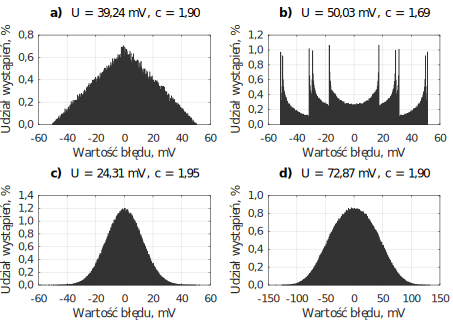
\includegraphics{obrazki/hist_part_S}
\makecaption{fig:symul_partd_hist_S_2_0}{Histogramy błędu \textbf{a)}~statycznego, \textbf{b)}~dynamicznego, \textbf{c)}~losowego, \textbf{d)}~wypadkowego, wielkości wyjściowej $S_{2,0}$ analizowanego w eksperymencie symulacyjnym toru pomiarowego uzyskane metodą Monte-Carlo}
\end{center}
\end{figure}

Na podstawie histogramów przedstawionych na rysunkach~\ref{fig:symul_partd_hist_S_2_0} oraz~\ref{fig:symul_partc_hist_T_1_0} zauważyć można, że oszacowane w równaniach od~\eqref{eq:sym_partd_output_unc_roun_S_2_0} do~\eqref{eq:sym_partd_output_unc_dyn_3_S_2_0} oraz od~\eqref{eq:sym_partd_output_unc_roun_T_1_0} do~\eqref{eq:sym_partd_output_unc_dyn_3_T_1_0} parametry sygnałów błędów pokrywają się z tymi uzyskanymi symulacyjnie. Współczynnik $A_{T_{1,0},s} $ określony w równaniu~\eqref{eq:sym_partd_output_as_T_1_0} wskazujący relacje pomiędzy wejściową i wyjściową wariancją błędów statycznych w przypadku wielkości wyjściowej $T_{1,0}$ jest w przybliżeniu równy zero. W rzeczywistości natomiast, ze względu na niewymierność kolejnych współczynników wiersza macierzy transformacji powiązanych z analizowaną wielkością wyjściową, współczynnik ten jest niezerowy. Fakt ten zauważyć można na podstawie rysunku~\ref{fig:symul_partc_hist_T_1_0}, gdzie teoretycznie wszystkie realizacje błędu statycznego powinny być zerowe. Omawiana rozbieżność jest jednak bardzo niewielka i nie wpływa zupełnie na uzyskane wyniki obliczeń.

\begin{figure}[htb!]
\begin{center}
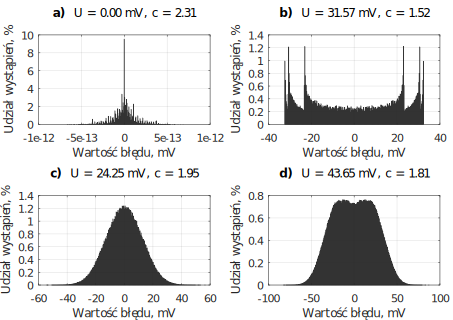
\includegraphics{obrazki/hist_part_T}
\makecaption{fig:symul_partc_hist_T_1_0}{Histogramy błędu \textbf{a)}~statycznego, \textbf{b)}~dynamicznego, \textbf{c)}~losowego, \textbf{d)}~wypadkowego, wielkości wyjściowej $T_{1,0}$ analizowanego w eksperymencie symulacyjnym toru pomiarowego uzyskane metodą Monte-Carlo}
\end{center}
\end{figure}

Ostatecznie wnioskować można, że przeprowadzony eksperyment wykazał poprawność zaproponowanej metody analizy oraz stworzonego na potrzeby pracy modelu błędu. Oszacowana przy użyciu proponowanej metody wartość wariancji dla analizowanych sygnałów każdorazowo okazywała się zbieżna z wartością uzyskaną metodą symulacyjną. Uzyskane wartości niepewności rozszerzonej, wyznaczane z użyciem redukcyjnej arytmetyki interwałowej, cechowały się rozbieżnością na poziomie mniejszym niż wymagany w założeniach pracy. Eksperyment wykazał możliwość stosowania uproszczenia obliczeń, które wynika bezpośrednio z warunków centralnego twierdzenia granicznego, natomiast stosowanie go dopuszczalne jest tylko i wyłącznie w określonych warunkach, natomiast w nieuzasadnionych przypadkach skutkować ono będzie przekraczającym~$\pm\qty{5}{\percent}$ błędem oszacowania niepewności rozszerzonej.

Identyczną analizę wykonano wykorzystując budżet niepewności zestawiony w tabeli~\ref{tab:sym_partc_params_unc_list}. Parametry kolejnych składowych sygnałów błędów wyznaczono analogicznie, jak miało to miejsce w przykładach opisanych zależnościami od~\eqref{eq:sym_partd_output_var_stat_S_2_0} do~\eqref{eq:sym_partd_output_var_dyn_3_S_2_0} oraz od~\eqref{eq:sym_partd_output_unc_stat_S_2_0} do~\eqref{eq:sym_partd_output_unc_dyn_3_S_2_0}. W tabelach~\ref{tab:sym_partd_params_unc_list_S_2_0} oraz~\ref{tab:sym_partd_params_unc_list_T_1_0} zestawiono budżety niepewności dla analizowanych wielkości wyjściowych $S_{2,0}$ oraz $T_{1,0}$.

\begin{table}[htb!]
\begin{center}
\makecaption{tab:sym_partd_params_unc_list_S_2_0}{Budżet niepewności wielkości wyjściowej $S_{2,0}$ analizowanego w eksperymencie symulacyjnym toru pomiarowego obejmujący wszystkie źródła błędów}
\begin{tabular}[c]{| c | c | S[table-format = 2.2] | S[table-format = 3.2] | c | c |} \hline
\textbf{Lp.} & \textbf{Symbol} & \textbf{$U$, mV} & \textbf{$\sigma^{2}$, \micro V} & \textbf{Rozkład} & \textbf{Źródło błędu} \\ \hline
1  & ${rw,z}$     & 2.13  &   0.97  & zaokrągleń                   & operacje zmiennoprzecinkowe                \\ \hline
2  & ${rp,q}$     & 13.26 &  45.78  & normalny                     & proces kwantowania (c)                     \\ \hline
3  & ${rp,1}$     & 11.80 &  36.26  & normalny                     & nieliniowość obiektu (a)                   \\ \hline
4  & ${rp,2}$     & 16.70 &  72.64  & normalny                     & szum wielkości wejściowej                  \\ \hline
5  & ${sp,1}$     & 23.04 &  147.00 & trójkątny                    & dryf temperatury (a)                       \\ \hline
6  & ${sp,2}$     & 16.29 &  73.52  & trójkątny                    & dryf temperatury (b)                       \\ \hline
7  & ${dp,a,1}$   & 12.32 &  76.40  & \multirow{6}{*}{dwumodalny}  & \multirow{3}{*}{transmitancja (a)}         \\ \cline{1-4}
8  & ${dp,a,2}$   & 25.08 &  316.38 &                              &                                            \\ \cline{1-4}
9  & ${dp,a,3}$   & 2.35  &  2.77   &                              &                                            \\ \cline{1-4} \cline{6-6}
10 & ${dp,b,1}$   & 6.07  &  18.52  &                              & \multirow{3}{*}{transmitancja (b)}         \\ \cline{1-4}
11 & ${dp,b,2}$   & 12.35 &  76.70  &                              &                                            \\ \cline{1-4}
12 & ${dp,b,3}$   & 1.16  &  0.67   &                              &                                            \\ \hline
\end{tabular}
\end{center}
\end{table}

\begin{table}[htb!]
\begin{center}
\makecaption{tab:sym_partd_params_unc_list_T_1_0}{Budżet niepewności wielkości wyjściowej $T_{1,0}$ analizowanego w eksperymencie symulacyjnym toru pomiarowego obejmujący wszystkie źródła błędów}
\begin{tabular}[c]{| c | c | S[table-format = 2.2] | S[table-format = 3.2] | c | c |} \hline
\textbf{Lp.} & \textbf{Symbol} & \textbf{$U$, mV} & \textbf{$\sigma^{2}$, \micro V} & \textbf{Rozkład} & \textbf{Źródło błędu} \\ \hline
1  & ${rw,z}$     & 1.81  &  0.70   & zaokrągleń                   & operacje zmiennoprzecinkowe                \\ \hline
2  & ${rp,q}$     & 13.26 &  45.78  & normalny                     & proces kwantowania (c)                     \\ \hline
3  & ${rp,1}$     & 11.80 &  36.26  & normalny                     & nieliniowość obiektu (a)                   \\ \hline
4  & ${rp,2}$     & 16.71 &  72.64  & normalny                     & szum wielkości wejściowej                  \\ \hline
5  & ${sp,1}$     & 0.00  &  0.00   & trójkątny                    & dryf temperatury (a)                       \\ \hline
6  & ${sp,2}$     & 0.00  &  0.00   & trójkątny                    & dryf temperatury (b)                       \\ \hline
7  & ${dp,a,1}$   & 0.06  &  0.00   & \multirow{6}{*}{dwumodalny}  & \multirow{3}{*}{transmitancja (a)}         \\ \cline{1-4}
8  & ${dp,a,2}$   & 3.77  &  7.13   &                              &                                            \\ \cline{1-4}
9  & ${dp,a,3}$   & 19.16 &  184.65 &                              &                                            \\ \cline{1-4} \cline{6-6}
10 & ${dp,b,1}$   & 0.03  &  0.00   &                              & \multirow{3}{*}{transmitancja (b)}         \\ \cline{1-4}
11 & ${dp,b,2}$   & 1.85  &  1.73   &                              &                                            \\ \cline{1-4}
12 & ${dp,b,3}$   & 9.44  &  44.82  &                              &                                            \\ \hline
\end{tabular}
\end{center}
\end{table}

Ze względu na korelacje wybranych sygnałów błędów wielkości wejściowych rozważanego algorytmu, wyznaczenie wypadkowych wartości wariancji sygnałów błędów dla kolejnych wielkości wyjściowych przeprowadzane jest zgodnie z zależnością~\eqref{eq:var_matrix}. W dalszej części rozważań przyjęto, że symbol $\bsigma_{*}$ oznacza wektor złożony z odchyleń standardowych sygnałów błędów składowych wielkości wyjściowej algorytmu, przy czym \enquote{$*$} oznacza symbol analizowanej wielkości wyjściowej. Macierz korelacji oznaczona symbolem $\mathbf{r}_{d}$ jest jednakowa dla wszystkich wielkości wyjściowych tego algorytmu i składa się z dwunastu wierszy i kolumn, co wynika z liczby analizowanych sygnałów błędów. Przyjmuje się, że kolejne wielkości zawarte w wektorze $\bsigma_{*}$ oraz kolejne elementy macierzy $\mathbf{r}_{d}$ są związane z sygnałami błędów zestawionymi w tabelach~\ref{tab:sym_partd_params_unc_list_S_2_0} oraz~\ref{tab:sym_partd_params_unc_list_T_1_0}, a dodatkowo kolejność wyrazów omawianych wielkości jest zgodna z tą daną w tabelach. Wobec powyższych, równanie~\eqref{eq:var_matrix} przyjmuje postać:
\begin{equation}
\sigma_{*,\Sigma}^{2} = \bsigma_{*}^{T} \cdot \mathbf{r}_{d} \cdot \bsigma_{*} \label{eq:sym_partd_output_varmat_list}.
\end{equation}

Uwzględniając pełną dodatnią korelacje pary sygnałów błędów statycznych wzmacniacza i przetwornika pomiarowego przyjmuje się, że $r_{d,sp,1,2} = 1$. Dodatkowo, na podstawie danych zawartych w tabelach~\ref{tab:sym_partb_params_dyn_self} oraz~\ref{tab:sym_partb_params_dyn_prop}, współczynniki korelacji kolejnych harmonicznych sygnału błędu dynamicznego o jednakowej częstotliwości są zbliżone do jedności, co wynika z równania~\eqref{eq:dyn_corr}, a zatem $r_{d,dp,a,b,n} = 1$ dla $n \in \{ 1, 2, 3 \}$. Wobec powyższych, kolejne elementy macierzy korelacji $\mathbf{r}_{d}$ przyjmują wartości:
\begin{equation}
\mathbf{r}_{d} =
\begin{bmatrix}
\num{1.0} & \num{0.0} & \num{0.0} & \num{0.0} & \num{0.0} & \num{0.0} & \num{0.0} & \num{0.0} & \num{0.0} & \num{0.0} & \num{0.0} & \num{0.0} \\
\num{0.0} & \num{1.0} & \num{0.0} & \num{0.0} & \num{0.0} & \num{0.0} & \num{0.0} & \num{0.0} & \num{0.0} & \num{0.0} & \num{0.0} & \num{0.0} \\
\num{0.0} & \num{0.0} & \num{1.0} & \num{0.0} & \num{0.0} & \num{0.0} & \num{0.0} & \num{0.0} & \num{0.0} & \num{0.0} & \num{0.0} & \num{0.0} \\
\num{0.0} & \num{0.0} & \num{0.0} & \num{1.0} & \num{0.0} & \num{0.0} & \num{0.0} & \num{0.0} & \num{0.0} & \num{0.0} & \num{0.0} & \num{0.0} \\
\num{0.0} & \num{0.0} & \num{0.0} & \num{0.0} & \num{1.0} & \num{1.0} & \num{0.0} & \num{0.0} & \num{0.0} & \num{0.0} & \num{0.0} & \num{0.0} \\
\num{0.0} & \num{0.0} & \num{0.0} & \num{0.0} & \num{1.0} & \num{1.0} & \num{0.0} & \num{0.0} & \num{0.0} & \num{0.0} & \num{0.0} & \num{0.0} \\
\num{0.0} & \num{0.0} & \num{0.0} & \num{0.0} & \num{0.0} & \num{0.0} & \num{1.0} & \num{0.0} & \num{0.0} & \num{1.0} & \num{0.0} & \num{0.0} \\
\num{0.0} & \num{0.0} & \num{0.0} & \num{0.0} & \num{0.0} & \num{0.0} & \num{0.0} & \num{1.0} & \num{0.0} & \num{0.0} & \num{1.0} & \num{0.0} \\
\num{0.0} & \num{0.0} & \num{0.0} & \num{0.0} & \num{0.0} & \num{0.0} & \num{0.0} & \num{0.0} & \num{1.0} & \num{0.0} & \num{0.0} & \num{1.0} \\
\num{0.0} & \num{0.0} & \num{0.0} & \num{0.0} & \num{0.0} & \num{0.0} & \num{1.0} & \num{0.0} & \num{0.0} & \num{1.0} & \num{0.0} & \num{0.0} \\
\num{0.0} & \num{0.0} & \num{0.0} & \num{0.0} & \num{0.0} & \num{0.0} & \num{0.0} & \num{1.0} & \num{0.0} & \num{0.0} & \num{1.0} & \num{0.0} \\
\num{0.0} & \num{0.0} & \num{0.0} & \num{0.0} & \num{0.0} & \num{0.0} & \num{0.0} & \num{0.0} & \num{1.0} & \num{0.0} & \num{0.0} & \num{1.0}
\end{bmatrix}
\label{eq:sym_partd_output_coher_list}.
\end{equation}

Zgodnie z zależnościami~\eqref{eq:sym_partd_output_varmat_list} oraz~\eqref{eq:sym_partd_output_coher_list}, po podstawieniu danych z tabel~\ref{tab:sym_partd_params_unc_list_S_2_0} oraz~\ref{tab:sym_partd_params_unc_list_T_1_0}, otrzymuje się wartości wariancji wypadkowych sygnałów błędów wielkości wyjściowych $S_{2,0}$ oraz $T_{1,0}$, przy czym kolejno:
\begin{gather}
\sigma_{S_{2,0},\Sigma}^{2} = \bsigma_{S_{2,0}}^{T} \cdot \mathbf{r}_{d} \cdot \bsigma_{S_{2,0}} = \qty{1464.79}{\micro V} \label{eq:sym_partd_output_varmat_S_2_0}, \\
\sigma_{T_{1,0},\Sigma}^{2} = \bsigma_{T_{1,0}}^{T} \cdot \mathbf{r}_{d} \cdot \bsigma_{T_{1,0}} = \qty{582.68}{\micro V} \label{eq:sym_partd_output_varmat_T_1_0}.
\end{gather}
Można zauważyć, że wyznaczone w ten sposób wartości są identyczne, jak te wyznaczone wcześniej w równaniach~\eqref{eq:sym_partd_output_var_sum_S_2_0} oraz~\eqref{eq:sym_partd_output_var_sum_T_1_0}.

Występowanie korelacji pomiędzy analizowanymi sygnałami błędów powoduje, że bezpośrednie zastosowanie metody opisanej równaniem~\eqref{eq:unc_matrix} dla współczynników koherencji wyznaczanych zgodnie z równaniem~\eqref{eq:unc_coher} nie jest możliwe. Aby umożliwić zastosowanie omawianej metody, proponuje się wyprowadzenie zależności opisujących wypadkowe parametry niepewności rozszerzonej dla grup skorelowanych sygnałów.

Dla sygnałów błędów statycznych wzmacniacza i przetwornika pomiarowego zapisać można następującą zależność, która określa wypadkową wartość niepewności rozszerzonej analizowanej pary sygnałów:
\begin{equation}
U_{*,sp} = \sqrt{
\begin{bmatrix}
U_{*,sp,1} \\ U_{*,sp,2}
\end{bmatrix}^{T}
\begin{bmatrix}
1 & h_{d,sp,1,2} \\
h_{d,sp,2,1} & 1
\end{bmatrix}
\begin{bmatrix}
U_{*,sp,1} \\ U_{*,sp,2}
\end{bmatrix}}
\label{eq:sym_partd_output_static_corrunc},
\end{equation}
przy czym w przypadku pełnej dodatniej korelacji tych sygnałów, tj. dla $r_{d,sp,1,2} = 1$, zachodzi $h_{d,sp,1,2} = 1$. Podobną zależność opisać można dla kolejnych par skorelowanych sygnałów błędów dynamicznych:
\begin{equation}
U_{*,dp,n} = \sqrt{
\begin{bmatrix}
U_{*,dp,a,n} \\ U_{*,dp,b,n}
\end{bmatrix}^{T}
\begin{bmatrix}
1 & h_{d,dp,a,b,n} \\
h_{d,dp,x,2,1} & 1
\end{bmatrix}
\begin{bmatrix}
U_{*,dp,a,n} \\ U_{*,dp,b,n}
\end{bmatrix}}
\label{eq:sym_partd_output_dynamic_corrunc},
\end{equation}
gdzie ze względu na pełną dodatnią korelację zachodzi $h_{d,dp,x,1,2} = 1$. W analizowanych przypadkach, opisanych równaniami~\eqref{eq:sym_partd_output_static_corrunc} oraz~\eqref{eq:sym_partd_output_dynamic_corrunc}, zauważyć można, że wypadkowe sygnały błędów cechować się będą identycznymi kształtami rozkładu, jak ich składowe.

Wobec powyższych, wektor niepewności rozszerzonych kolejnych sygnałów błędów dla wielkości wyjściowych analizowanego toru pomiarowego przedstawić można jako:
\begin{equation}
\mathbf{U}_{*} =
\begin{bmatrix}
U_{*,rw,z} & U_{*,rp,q} & U_{*,rp,1} & U_{*,rp,2} & U_{*,sp} & U_{*,dp,1} & U_{*,dp,2} & U_{*,dp,3}
\end{bmatrix}
\label{eq:sym_partd_output_unc_sumuvect},
\end{equation}
natomiast macierz koherencji, której wartości wyznaczane są zgodnie z równaniem~\eqref{eq:unc_coher}, opisać można dla kolejnych wielkości wyjściowych w postaci:
\begin{equation}
\mathbf{h}_{*} =
\begin{bmatrix}
1 & h_{*,0,1} & h_{*,0,2} & h_{*,0,3} & h_{*,0,4} & h_{*,0,5} & h_{*,0,6} & h_{*,0,7} \\
h_{*,1,0} & 1 & h_{*,1,2} & h_{*,1,3} & h_{*,1,4} & h_{*,1,5} & h_{*,1,6} & h_{*,1,7} \\
h_{*,2,0} & h_{*,2,1} & 1 & h_{*,2,3} & h_{*,2,4} & h_{*,2,5} & h_{*,2,6} & h_{*,2,7} \\
h_{*,3,0} & h_{*,3,1} & h_{*,3,2} & 1 & h_{*,3,4} & h_{*,3,5} & h_{*,3,6} & h_{*,3,7} \\
h_{*,4,0} & h_{*,4,1} & h_{*,4,2} & h_{*,4,3} & 1 & h_{*,4,5} & h_{*,4,6} & h_{*,4,7} \\
h_{*,5,0} & h_{*,5,1} & h_{*,5,2} & h_{*,5,3} & h_{*,5,4} & 1 & h_{*,5,6} & h_{*,5,7} \\
h_{*,6,0} & h_{*,6,1} & h_{*,6,2} & h_{*,6,3} & h_{*,6,4} & h_{*,6,5} & 1 & h_{*,6,7} \\
h_{*,7,0} & h_{*,7,1} & h_{*,7,2} & h_{*,7,3} & h_{*,7,4} & h_{*,7,5} & h_{*,7,6} & 1
\end{bmatrix}
\label{eq:sym_partd_output_unc_cohermat},
\end{equation}
przy czym kolejność elementów przedstawionej macierzy odpowiada kolejności elementów w wektorze niepewności rozszerzonych, opisanym równaniem~\eqref{eq:sym_partd_output_unc_sumuvect}, gdzie przykładowo $h_{*,0,1} = h_{*,rw,z,rp,q}$. Ostatecznie, wartość wypadkowej niepewności rozszerzonej może być oszacowana zgodnie z równaniem~\eqref{eq:unc_matrix}:
\begin{equation}
U_{*} = \sqrt{\mathbf{U}_{*} \cdot \mathbf{h}_{*} \cdot \mathbf{U}_{*}^{T}} \label{eq:sym_partd_output_unc_totalmat}.
\end{equation}

Podstawiając do równania~\eqref{eq:sym_partd_output_static_corrunc} wartości z tabel~\ref{tab:sym_partd_params_unc_list_S_2_0} oraz~\ref{tab:sym_partd_params_unc_list_T_1_0} otrzymuje się wypadkowe wartości niepewności rozszerzonej dla sygnałów wypadkowych skorelowanych błędów statycznych wielkości $S_{2,0}$ oraz $T_{1,0}$ w postaci:
\begin{gather}
\begin{split}
U_{S_{2,0},sp} = & \sqrt{
\begin{bmatrix}
U_{S_{2,0},sp,1} \\ U_{S_{2,0},sp,2}
\end{bmatrix}^{T}
\begin{bmatrix}
1 & h_{d,sp,1,2} \\
h_{d,sp,2,1} & 1
\end{bmatrix}
\begin{bmatrix}
U_{S_{2,0},sp,1} \\ U_{S_{2,0},sp,2}
\end{bmatrix}} = \\ & \sqrt{
\begin{bmatrix}
\num{23.04e-3} \\ \num{16.29e-3}
\end{bmatrix}^{T}
\begin{bmatrix}
1 & 1 \\
1 & 1
\end{bmatrix}
\begin{bmatrix}
\num{23.04e-3} \\ \num{16.29e-3}
\end{bmatrix}} = \qty{39.31}{mV}
\end{split}
\label{eq:sym_partd_output_static_corrunc_S_2_0}, \\
\begin{split}
U_{T_{1,0},sp} = & \sqrt{
\begin{bmatrix}
U_{T_{1,0},sp,1} \\ U_{T_{1,0},sp,2}
\end{bmatrix}^{T}
\begin{bmatrix}
1 & h_{d,sp,1,2} \\
h_{d,sp,2,1} & 1
\end{bmatrix}
\begin{bmatrix}
U_{T_{1,0},sp,1} \\ U_{T_{1,0},sp,2}
\end{bmatrix}} = \\ & \sqrt{
\begin{bmatrix}
\num{0.00} \\ \num{0.00}
\end{bmatrix}^{T}
\begin{bmatrix}
1 & 1 \\
1 & 1
\end{bmatrix}
\begin{bmatrix}
\num{0.00} \\ \num{0.00}
\end{bmatrix}} = \qty{0.00}{mV}
\end{split}
\label{eq:sym_partd_output_static_corrunc__T_1_0},
\end{gather}
natomiast w przypadku równania~\eqref{eq:sym_partd_output_dynamic_corrunc} dla pierwszej harmonicznej sygnałów błędów dynamicznych omawianych wielkości zachodzi:
\begin{gather}
\begin{split}
U_{S_{2,0},dp,1} = & \sqrt{
\begin{bmatrix}
U_{S_{2,0},dp,a,1} \\ U_{S_{2,0},dp,b,1}
\end{bmatrix}^{T}
\begin{bmatrix}
1 & h_{d,dp,a,b,1} \\
h_{d,dp,b,a,1} & 1
\end{bmatrix}
\begin{bmatrix}
U_{S_{2,0},dp,a,1} \\ U_{S_{2,0},dp,b,1}
\end{bmatrix}} = \\ & \sqrt{
\begin{bmatrix}
\num{12.32e-3} \\ \num{6.07e-3}
\end{bmatrix}^{T}
\begin{bmatrix}
1 & 1 \\
1 & 1
\end{bmatrix}
\begin{bmatrix}
\num{12.32e-3} \\ \num{6.07e-3}
\end{bmatrix}} = \qty{18.39}{mV}
\end{split}
\label{eq:sym_partd_output_dynamic_corrunc_S_2_0}, \\
\begin{split}
U_{T_{1,0},dp,1} = & \sqrt{
\begin{bmatrix}
U_{T_{1,0},dp,a,1} \\ U_{T_{1,0},dp,b,1}
\end{bmatrix}^{T}
\begin{bmatrix}
1 & h_{d,dp,a,b,1} \\
h_{d,dp,b,a,1} & 1
\end{bmatrix}
\begin{bmatrix}
U_{T_{1,0},dp,a,1} \\ U_{T_{1,0},dp,b,1}
\end{bmatrix}} = \\ & \sqrt{
\begin{bmatrix}
\num{0.06e-3} \\ \num{0.03e-3}
\end{bmatrix}^{T}
\begin{bmatrix}
1 & 1 \\
1 & 1
\end{bmatrix}
\begin{bmatrix}
\num{0.06e-3} \\ \num{0.03e-3}
\end{bmatrix}} = \qty{0.092}{mV}
\end{split}
\label{eq:sym_partd_output_dynamic_corrunc_T_1_0}.
\end{gather}
Parametry pozostałych harmonicznych sygnałów błędów dynamicznych wyznaczono w analogiczny sposób, zatem obliczenia z nimi związane nie zastały przedstawione. Po podstawieniu uzyskanych wyników do równania~\eqref{eq:sym_partd_output_unc_sumuvect} otrzymuje się wektory składowych niepewności rozszerzonych dla analizowanych wielkości wyjściowych:
\begin{gather}
\mathbf{U}_{S_{2,0}} =
\begin{bmatrix}
\num{2.13} & \num{13.26} & \num{11.80} & \num{16.71} & \num{39.33} & \num{18.39} & \num{37.42} & \num{3.50}
\end{bmatrix} \cdot \num{e-3}
\label{eq:sym_partd_output_unc_sumuvect_S_2_0_b}, \\
\mathbf{U}_{T_{1,0}} =
\begin{bmatrix}
\num{1.81} & \num{13.26} & \num{11.80} & \num{16.71} & \num{0.00} & \num{0.092} & \num{5.62} & \num{28.60}
\end{bmatrix} \cdot \num{e-3}
\label{eq:sym_partd_output_unc_sumuvect_T_1_0_b},
\end{gather}
przy czym kolejne wyrazy macierzy koherencji dla analizowanych wielkości wyjściowych wyznaczane są zgodnie z równaniem~\eqref{eq:unc_coher}, a zatem przyjmują wartości:
\begin{gather}
\mathbf{h}_{S_{2,0}} =
\begin{bmatrix}
1 & h_{*,0,1} & h_{*,0,2} & h_{*,0,3} & h_{*,0,4} & h_{*,0,5} & h_{*,0,6} & h_{*,0,7} \\
h_{*,1,0} & 1 & h_{*,1,2} & h_{*,1,3} & h_{*,1,4} & h_{*,1,5} & h_{*,1,6} & h_{*,1,7} \\
h_{*,2,0} & h_{*,2,1} & 1 & h_{*,2,3} & h_{*,2,4} & h_{*,2,5} & h_{*,2,6} & h_{*,2,7} \\
h_{*,3,0} & h_{*,3,1} & h_{*,3,2} & 1 & h_{*,3,4} & h_{*,3,5} & h_{*,3,6} & h_{*,3,7} \\
h_{*,4,0} & h_{*,4,1} & h_{*,4,2} & h_{*,4,3} & 1 & h_{*,4,5} & h_{*,4,6} & h_{*,4,7} \\
h_{*,5,0} & h_{*,5,1} & h_{*,5,2} & h_{*,5,3} & h_{*,5,4} & 1 & h_{*,5,6} & h_{*,5,7} \\
h_{*,6,0} & h_{*,6,1} & h_{*,6,2} & h_{*,6,3} & h_{*,6,4} & h_{*,6,5} & 1 & h_{*,6,7} \\
h_{*,7,0} & h_{*,7,1} & h_{*,7,2} & h_{*,7,3} & h_{*,7,4} & h_{*,7,5} & h_{*,7,6} & 1
\end{bmatrix}
\label{eq:sym_partd_output_unc_cohermat_S_2_0_b}, \\
\mathbf{h}_{T_{1,0}} =
\begin{bmatrix}
1 & h_{*,0,1} & h_{*,0,2} & h_{*,0,3} & h_{*,0,4} & h_{*,0,5} & h_{*,0,6} & h_{*,0,7} \\
h_{*,1,0} & 1 & h_{*,1,2} & h_{*,1,3} & h_{*,1,4} & h_{*,1,5} & h_{*,1,6} & h_{*,1,7} \\
h_{*,2,0} & h_{*,2,1} & 1 & h_{*,2,3} & h_{*,2,4} & h_{*,2,5} & h_{*,2,6} & h_{*,2,7} \\
h_{*,3,0} & h_{*,3,1} & h_{*,3,2} & 1 & h_{*,3,4} & h_{*,3,5} & h_{*,3,6} & h_{*,3,7} \\
h_{*,4,0} & h_{*,4,1} & h_{*,4,2} & h_{*,4,3} & 1 & h_{*,4,5} & h_{*,4,6} & h_{*,4,7} \\
h_{*,5,0} & h_{*,5,1} & h_{*,5,2} & h_{*,5,3} & h_{*,5,4} & 1 & h_{*,5,6} & h_{*,5,7} \\
h_{*,6,0} & h_{*,6,1} & h_{*,6,2} & h_{*,6,3} & h_{*,6,4} & h_{*,6,5} & 1 & h_{*,6,7} \\
h_{*,7,0} & h_{*,7,1} & h_{*,7,2} & h_{*,7,3} & h_{*,7,4} & h_{*,7,5} & h_{*,7,6} & 1
\end{bmatrix}
\label{eq:sym_partd_output_unc_cohermat_T_1_0_b}.
\end{gather}
Po podstawieniu powyższych wartości do równania~\eqref{eq:sym_partd_output_unc_totalmat} otrzymuje się wartości wypadkowych niepewności rozszerzonych analizowanych wielkości wyjściowych toru pomiarowego, gdzie kolejno:
\begin{gather}
U_{S_{2,0}} = \sqrt{\mathbf{U}_{S_{2,0}} \cdot \mathbf{h}_{S_{2,0}} \cdot \mathbf{U}_{S_{2,0}}^{T}} = \qty{74.10}{mV} \label{eq:sym_partd_output_unc_totalmat_S_2_0}, \\
U_{T_{1,0}} = \sqrt{\mathbf{U}_{T_{1,0}} \cdot \mathbf{h}_{T_{1,0}} \cdot \mathbf{U}_{T_{1,0}}^{T}} = \qty{43.37}{mV} \label{eq:sym_partd_output_unc_totalmat_T_1_0}.
\end{gather}

Przedstawione w równaniach~\eqref{eq:sym_partd_output_unc_totalmat_S_2_0} oraz~\eqref{eq:sym_partd_output_unc_totalmat_T_1_0} obliczenia wykonano ponownie, dla macierzy koherencji których wartości wyznaczone zostały bez uwzględnienia korekty zaproponowanej w równaniu~\eqref{eq:unc_cohercorra}, tj. kiedy w równaniu~\eqref{eq:unc_coher} przyjmuje się $p_{i,j} = 1$ dla dowolnej pary $i$ oraz $j$. Otrzymane wartości wyniosły kolejno $U_{S_{2,0}} = \qty{77.32}{mV}$ oraz $U_{T_{1,0}} = \qty{46.09}{mV}$. Podobne obliczenia wykonano dla pozostałych wielkości wyjściowych.

W tabeli~\ref{tab:sym_partd_params_unc_sum_b} zestawiono wyniki obliczeń dla pozostałych wielkości wyjściowych oraz te uzyskane w poprzednim eksperymencie, w celu umożliwienia ich porównania. Symbolem $a$ oznaczono wartości uzyskane przy założeniu normalnego rozkładu sygnału błędu wypadkowego, symbolem $b$ oznaczono wartości uzyskane z wykorzystaniem budżetu niepewności opisanego w tabeli~\ref{tab:sym_partc_params_unc_sum}. Wartości oznaczone symbolem $c$ dotyczą analizy z wykorzystaniem budżetu niepewności opisanego w tabeli~\ref{tab:sym_partc_params_unc_list}, przy czym wielkości oznaczone symbolem $d$ wyznaczono identycznie, jak dla $c$, z tą różnicą że nie stosowano korekty opisanej równaniem~\eqref{eq:unc_cohercorra} w procesie wyznaczania wartości współczynników koherencji. Podobnie, jak w zestawieniu zawartym w tabeli~\ref{tab:sym_partd_params_unc_sum_a}, wielkości oznaczone symbolem $s$ dotyczą przeprowadzonego eksperymentu metodą Monte-Carlo, natomiast symbolem $\delta_{*}$ oznaczono błąd względny oszacowania wartości niepewności rozszerzonej metodą $a$, $b$, $c$ oraz $d$ w odniesieniu do wartości $U_{s}$, wyrażony w procentach, wyznaczany zgodnie z zależnością~\eqref{eq:unc_error}.

\begin{table}[htb!]
\begin{center}
\makecaption{tab:sym_partd_params_unc_sum_b}{Porównanie uzyskanych przedstawionymi w pracy metodami wartości wypadkowych niepewności rozszerzonych kolejnych wielkości wyjściowych analizowanego w eksperymencie symulacyjnym toru pomiarowego}
\begin{tabular}[c]{| c *{5}{|S[table-format = 2.2]} *{4}{|S[table-format = +1.2]} |} \hline
\multirow{2}{*}{\textbf{Wielkość}} & \multicolumn{5}{c|}{\textbf{Niepewność, mV}} & \multicolumn{4}{c|}{\textbf{Błąd, \%}} \\ \cline{2-10}
& $U_{a}$ & $U_{b}$ & $U_{c}$ & $U_{d}$ & $U_{s}$ & $\delta_{a}$ & $\delta_{b}$ & $\delta_{c}$ & $\delta_{d}$ \\ \hline
$S_{2,0}$ & 75.01 & 74.00 & 74.10 & 77.32 & 72.87 & +2.94 & +1.55 & +1.69 & +6.11 \\ \hline
$S_{2,1}$ & 68.19 & 68.44 & 68.43 & 71.52 & 67.09 & +1.64 & +2.01 & +2.00 & +6.60 \\ \hline
$T_{2,0}$ & 57.29 & 56.26 & 55.91 & 57.58 & 53.89 & +6.31 & +4.40 & +3.75 & +6.85 \\ \hline
$T_{2,1}$ & 58.86 & 55.59 & 55.60 & 59.47 & 54.92 & +7.17 & +1.22 & +1.24 & +8.28 \\ \hline
$T_{1,0}$ & 47.31 & 43.61 & 43.37 & 46.09 & 43.76 & +8.11 & -0.34 & -0.89 & +5.32 \\ \hline
$T_{1,1}$ & 47.31 & 43.60 & 43.37 & 46.08 & 43.74 & +8.16 & -0.32 & -0.85 & +5.35 \\ \hline
$T_{1,2}$ & 47.31 & 43.60 & 43.37 & 46.08 & 43.76 & +8.11 & -0.37 & -0.89 & +5.30 \\ \hline
$T_{1,3}$ & 44.79 & 43.64 & 43.39 & 45.43 & 43.17 & +3.75 & +1.09 & +0.51 & +5.24 \\ \hline
\end{tabular}
\end{center}
\end{table}

Analizując wyniki przedstawione w tabeli~\ref{tab:sym_partd_params_unc_sum_b} zauważyć można, że zaproponowana w pracy metoda szacowania wypadkowej wartości niepewności rozszerzonej wraz z zastosowaniem proponowanego modelu błędu zapewniają wyniki zbieżne z tymi uzyskanymi symulacyjnie. Korekta wartości współczynników koherencji opisana równaniem~\eqref{eq:unc_cohercorra} pozwala na znaczne zmniejszenie rozbieżności pomiędzy szacowaną zgodnie z równaniem~\eqref{eq:unc_matrix} wartością, a wartością uzyskiwaną symulacyjnie, w stosunku do wartości uzyskanych bez stosowania opisanej korekty. Wartości uzyskane przy zastosowaniu budżetu niepewności zawierającego jedynie wypadkowe parametry sygnałów błędów z uwzględnieniem na wprowadzone kategorie błędów są zbieżne z wartościami uzyskanymi dla budżetu obejmującego charakterystykę każdego z sygnałów błędów. Rozbieżności pomiędzy wartościami oznaczonymi symbolami $b$ oraz $c$ wynikają z innego oszacowania wartości współczynników koherencji.

\section{Podsumowanie przeprowadzonego eksperymentu}

Przedstawione w bieżącym rozdziale rozważania i przeprowadzone eksperymenty potwierdzają poprawność proponowanego w pracy modelu błędu oraz skuteczność stosowanej metody redukcyjnej arytmetyki interwałowej. Oszacowane zgodnie z równaniem~\eqref{eq:unc_matrix} wartości wypadkowej niepewności rozszerzonej dla współczynników koherencji szacowanych zgodnie z zależnością~\eqref{eq:unc_coher} każdorazowo okazywały się zbieżne z wynikami uzyskiwanymi dla przeprowadzonych metodą Monte-Carlo eksperymentów. Wartości niepewności oszacowane stosując zaproponowaną w pracy korektę wartości współczynników koherencji daną równaniem~\eqref{eq:unc_cohercorra} były bliższe uzyskanym eksperymentalnie, natomiast w praktyce pomiarowej korekta ta nie jest wymagana, jeżeli dopuszcza się przekraczający~\qty{5}{\percent} błąd oszacowania wartości wypadkowej niepewności rozszerzonej. Należy również brać pod uwagę, że oszacowane w proponowany sposób wartości niepewności rozszerzonej mogą być w pewnych przypadkach nieco niższe, niż wartości prawdziwe. Różnice te nie przekraczają jednak~\qty{-3}{\percent} wartości prawdziwej, co wykazano w eksperymencie, którego wyniki przedstawiono wcześniej na rysunku~\ref{fig:hist_reductive} oraz w przedstawionych dotychczas rozważaniach.

W przypadku, gdy analizowane sygnały błędów składowych cechować się będą nietypowym rozkładem, stosowanie omawianej w pracy metody wymagać będzie wyznaczenia wartości współczynników kształtu dla wszystkich analizowanych typów rozkładów. Jest to jedyna czynność, której przeprowadzenie nie będzie mogło zwykle odbywać się w czasie pracy systemu pomiarowego i będzie musiała zostać przeprowadzona na etapie identyfikacji jego właściwości. Podobny problem napotkać można w przypadku wystąpienia korelacji pomiędzy analizowanymi sygnałami błędów składowych -- należy wtedy postąpić identycznie, jak pokazano w przykładzie lub zastosować inną metodę wyznaczania wartości elementów macierzy koherencji, jak chociażby pokazano w pracy~\cite{jakubiec_reductive}.

Przedstawiona w równaniach od~\eqref{eq:sym_partd_output_static_corrunc} do~\eqref{eq:sym_partd_output_unc_totalmat} analiza umożliwiła wykorzystanie zaproponowanej metody szacowania wartości współczynników koherencji, opisanej równaniem~\eqref{eq:unc_coher} mimo, że metoda ta nie jest odpowiednia dla analizy skorelowanych sygnałów. Możliwość zastosowania opisanego algorytmu wynika z faktu, że wypadkowe sygnały dla skorelowanych grup sygnałów cechują się typowym kształtem rozkładu, dla którego wyznaczono wcześniej wartości współczynników kształtu. W innych okolicznościach należałoby wyznaczyć odpowiednie dla analizowanych parametrów sygnałów wartości współczynników koherencji.

Jako, że żaden z etapów szacowania wypadkowej wartości niepewności rozszerzonej zgodnie z zaproponowaną metodą nie wymaga przeprowadzania dodatkowych symulacji metodą Monte-Carlo, a wykonywane obliczenia sprowadzają się do prostych operacji arytmetycznych, przedstawiona metoda może zostać zaimplementowana w torze pomiarowym w celu bieżącej oceny jego właściwości metrologicznych. W przypadku zmiany parametrów sygnałów błędów obecnych w analizowanym torze pomiarowym wymagane jest jedynie ponowne wyznaczenie wartości macierzy koherencji i wskazanie parametrów istniejących sygnałów błędów. Istotnymi parametrami analizowanych sygnałów błędów jest w tym przypadku wartość niepewności rozszerzonej dla wybranego, identycznego dla wszystkich wielkości poziomu ufności oraz rodzaj rozkładu analizowanego sygnału.

Stosowanie uproszczenia, gdzie zakłada się normalny rozkład błędu wypadkowego, pozwala znacznie uprościć proces wyznaczania wypadkowej wartości niepewności rozszerzonej i zastąpić konieczność stosowania zależności~\eqref{eq:unc_matrix} oraz~\eqref{eq:unc_coher} wyznaczeniem wariancji wypadkowego sygnału błędu, natomiast jego stosowanie wymaga posiadania pewności odnoście spełnienia warunków centralnego twierdzenia granicznego. Jak wykazały przeprowadzone eksperymenty, nawet dla kilkunastu źródeł błędów, gdzie większość z nich nie jest wzajemnie skorelowana, założenie to może okazać się niespełnione, co skutkuje znaczną rozbieżnością pomiędzy oszacowaną, a prawdziwą wartością niepewności rozszerzonej na poziomie zbliżonym do~\qty{10}{\percent}.

Mimo, że wprowadzenie do proponowanego modelu błędu funkcji przetwarzania obiektu może być zastąpione wprowadzeniem statycznego wzmocnienia w równaniu transmitancji obiektu, obecność tej funkcji umożliwia bardziej spójną w logiczną analizę rzeczywistych obiektów. Nawet, jeśli rzeczywista postać funkcji przetwarzania nie jest znana, to wprowadzany przez nią sygnał błędu można opisać odpowiednią zależnością lub wskazać jego parametry, jak pokazano w omówionym przykładzie. Przeprowadzone badania wykazały, że w przypadku nieznanej rzeczywistej funkcji przetwarzania obiektu do oszacowania wpływu tej funkcji na postać sygnałów na wyjściu obiektu, wykorzystać można idealne równanie funkcji przetwarzania. Omawiana okoliczność jest bardzo cenna w przypadku nieliniowości charakterystyki obiektu lub analizy przetwornika analogowo-cyfrowego.
